\documentclass[17pt,a4paper,oneside,margin=1in]{article}
\usepackage[utf8]{inputenc}
\usepackage{graphicx}
\usepackage{fontspec}
\usepackage{subfigure}
\usepackage{pdfpages}
\setmainfont{times-new-roman.ttf}
\begin{document}
\pagestyle{empty}
\begin{figure}[tp] % inserting CDCSIT Logo
\centering

\includegraphics[width=90pt]{./scrot/logo.png}
\end{figure}
\begin{center}
 {\Large \textbf{{Lab Assignment for Introduction to Information Technology}}}\par
 {\large \textbf{{A Project Report}\\}}
\begin{figure}[hbtp]
 \centering

\includegraphics[width=45pt,height=100pt]{./scrot/vlines.png}
\end{figure}
  {\Large \textbf{{Submitted By}\\}}
  {\Large Anukul Adhikari\\\large Roll No. 10\\ \large Date: {\today}}\par        
{\Large \textbf{{Submitted To}\\}}
{\large Department of Computer Science and Information Technology\\ Bhaktapur Multiple Campus \\
					Doodhpati, Bhaktapur, Nepal }\par					
{\Large\vspace*{5mm} \textbf {Under the Supervision of}\\
			\vspace*{3mm}\large Mr. Surya Bam}\par 
\end{center}

\tableofcontents
\pagestyle{plain}

\pagebreak

\section*{Acknowledgements}
%\addcontentsline{toc}{chapter{Acknowledgments}}
%\protect\thispagestyle{empty}

All thanks to my adorable parents for their profound help and support during the cause of this project work.Without constant guidance and suggestions, this report would have been nowhere near completion.Finally, I thank to all my teachers and friends, who were the people, who prepared me for this endeavor. I own you all my success

\clearpage
\section{Intro To DOS} 
%\addcontentsline{toc}{chapter{Intro To DOS}}
%\protect\thispagestyle{empty}
In the personal computer operating systems MS-DOS and PC DOS, a number of standard system commands were provided for common tasks such as listing files on a disk or moving files. Some commands were built into the command interpreter, others existed as external commands on disk. Over the several generations of DOS, commands were added for the additional functions of the operating system. In the current Microsoft Windows operating system a text-mode command prompt window can still be used. 
The command interpreter for DOS runs when no application programs are running. When an application exits, if the transient portion of the command interpreter in memory was overwritten, DOS will reload it from disk. Some commands are internal and built into COMMAND.COM, others are external commands stored on disk. When the user types a line of text at the operating system command prompt, COMMAND.COM will parse the line and attempt to match a command name to a built-in command or to the name of an executable program file or batch file on disk. If no match is found, an error message is printed and the command prompt is refreshed.
\section{Different types of DOS commands}


\subsection{DIR}
This commands lists all directory and filed from given directory. \\
Syntax:\\
\begin{verbatim}
	DIR [pathname][display_format][file_attributes][sorted][time][options]
\end{verbatim}
\begin{figure}[h]
	\caption{Example of a DIR command on DOSBOX}
	\centering
	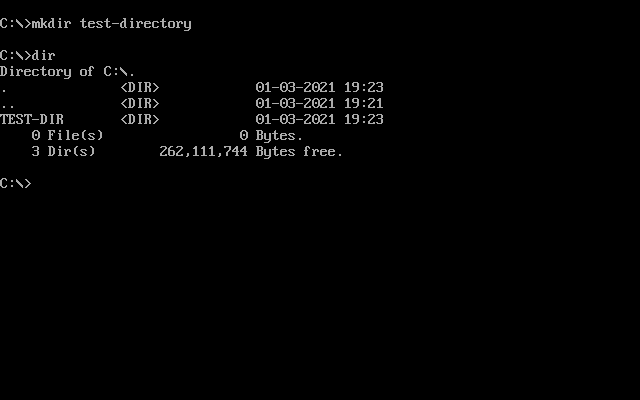
\includegraphics[width=1\textwidth]{./scrot/dir.png}
\end{figure}
\pagebreak


\subsection{MKDIR}
This command created directory in given path. \\
Syntax: \\
\begin{verbatim}
	DIR DRIVE:\path] [DRIVE:\path]	
\end{verbatim}
\begin{figure}[h]
	\caption{Example of a MKDIR command on DOSBOX}
	\centering
	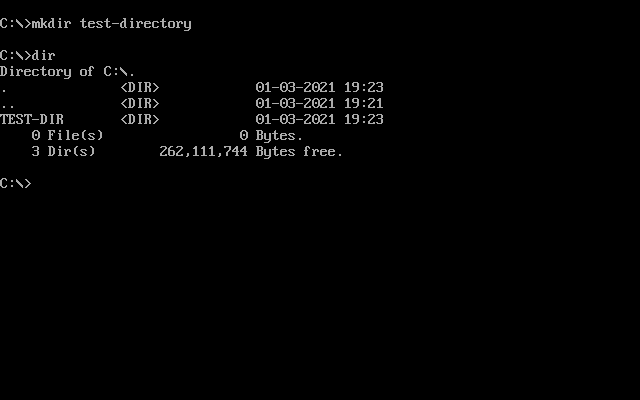
\includegraphics[width=1\textwidth]{./scrot/dir.png}
\end{figure}
\pagebreak


\subsection{CD}
This command changes directory to given path. \\
Syntax: \\
\begin{verbatim}
	CD [\path] 	
\end{verbatim}
\begin{figure}[h]
	\caption{Example of a CD command on DOSBOX}
	\centering
	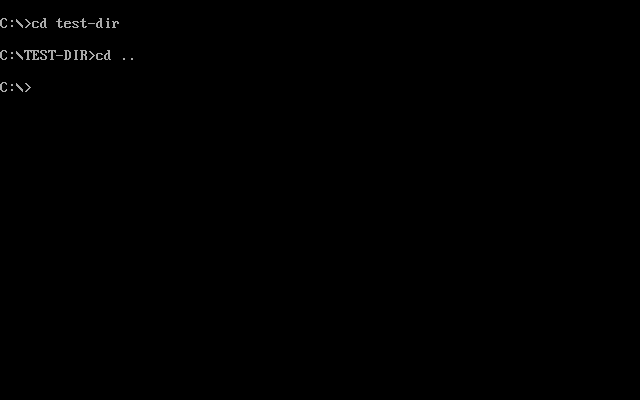
\includegraphics[width=1\textwidth]{./scrot/cd.png}
\end{figure}
\pagebreak


\subsection{TYPE}
This command prints out the contents of the file(s) from given path. \\
Syntax: \\
\begin{verbatim}
	TYPE [\path\filename] 	
\end{verbatim}
\begin{figure}[h]
	\caption{Example of a TYPE command on DOSBOX}
	\centering
	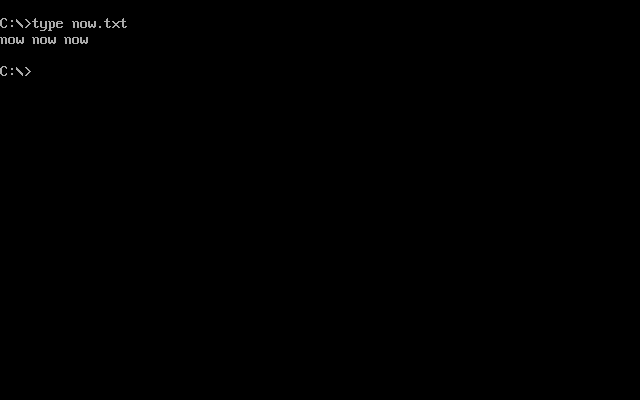
\includegraphics[width=1\textwidth]{./scrot/type.png}
\end{figure}
\pagebreak


\subsection{ECHO}
This command echoes out the text written after the first argument(echo itself) and prints to stdout.
Echo serves multipurpose function, when paired with pipe command it writes to file the contents that was supposed to be echoed to stdout.\\
Syntax: \\
\begin{verbatim}
	ECHO "...some text..."  	
\end{verbatim}
\begin{figure}[h]
	\caption{Example of a ECHO command on DOSBOX}
	\centering
	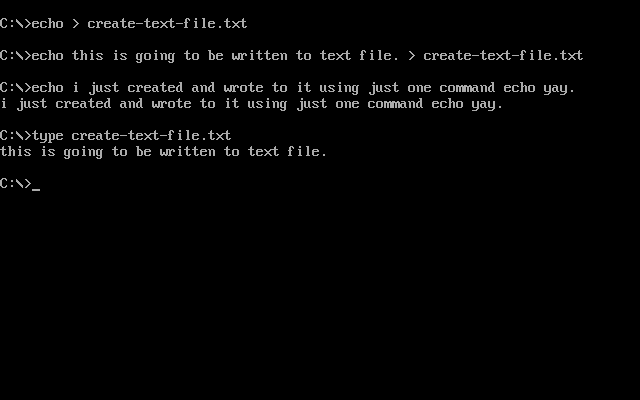
\includegraphics[width=1\textwidth]{./scrot/echo.png}
\end{figure}
\pagebreak


\subsection{COPY}
This command copies the file from one location to another, meanwhile it can be used to rename file too.\\
Syntax: \\
\begin{verbatim}
	COPY [path\source\filename.extension][path\destination\filename.extension]  	
\end{verbatim}
\begin{figure}[h]
	\caption{Example of a COPY command on DOSBOX}
	\centering
	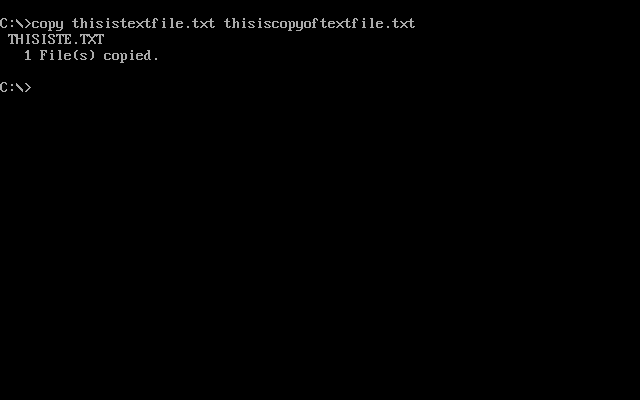
\includegraphics[width=1\textwidth]{./scrot/copy.png}
\end{figure}
\pagebreak


\subsection{MEM}
This command displays the amount of installed and available memory, including extending, expanded, and upper memory.\\
Syntax: \\
\begin{verbatim}
	MEM [/program|/debug|/classify|/free|/module(name)][/page]
\end{verbatim}
\begin{figure}[h]
	\caption{Example of a MEM command on DOSBOX}
	\centering
	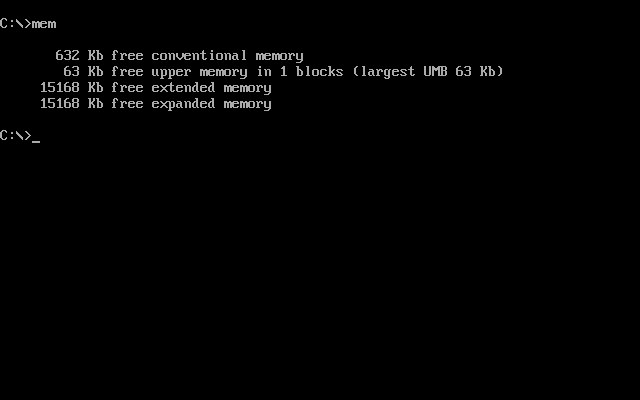
\includegraphics[width=1\textwidth]{./scrot/mem.png}
\end{figure}
\pagebreak


\subsection{DEL}
This command deletes the file from given path.\\
Syntax: \\
\begin{verbatim}
	DEL [\path\filename.extension]
\end{verbatim}
\begin{figure}[h]
	\caption{Example of a DEL command on DOSBOX}
	\centering
	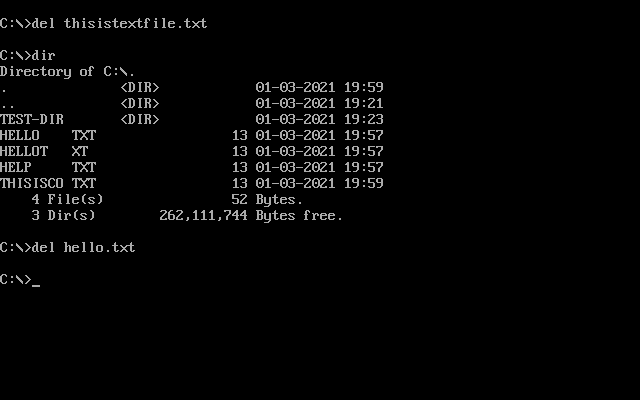
\includegraphics[width=1\textwidth]{./scrot/del.png}
\end{figure}
\pagebreak


\subsection{CLS}
This command clears all previous command output from the screen.\\
Syntax: \\
\begin{verbatim}
	CLS
\end{verbatim}
\begin{figure}[ht]
	\begin{subfigure}
		\centering
		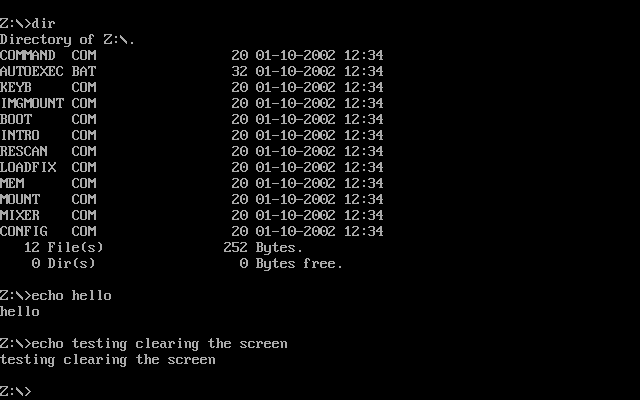
\includegraphics[width=0.8\linewidth]{./scrot/cls1.png}
		\caption{Example before using CLS command on DOSBOX}
		\label{fig:sub-first}
	\end{subfigure}
	\begin{subfigure}
		\centering
		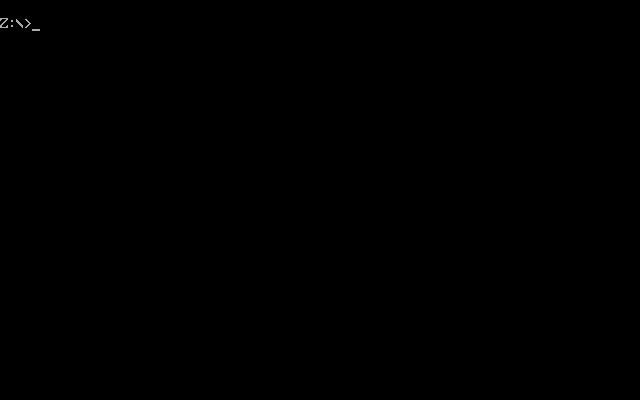
\includegraphics[width=0.8\linewidth]{./scrot/cls2.png}
		\caption{Example after using CLS command on DOSBOX}
		\label{fig:sub-second}
	\end{subfigure}
\end{figure}
\pagebreak


\subsection{HELP}
This command shows all the files that can be used in DOS.\\
Syntax: \\
\begin{verbatim}
	HELP	
\end{verbatim}
\begin{figure}[h]
	\caption{Example of a HELP command on DOSBOX}
	\centering
	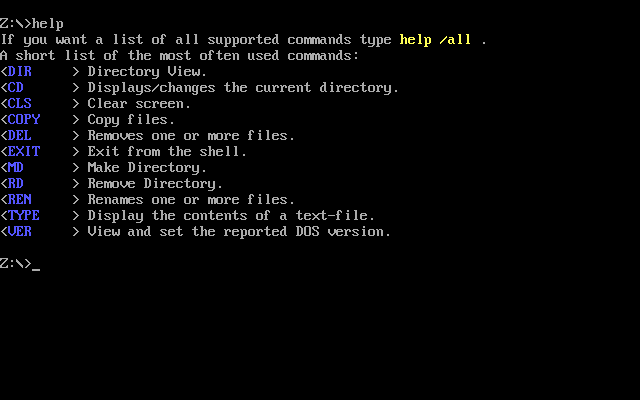
\includegraphics[width=1\textwidth]{./scrot/help.png}
\end{figure}
\pagebreak

\section{Project Work On Word Processor}
\subsection{Bio-Data}
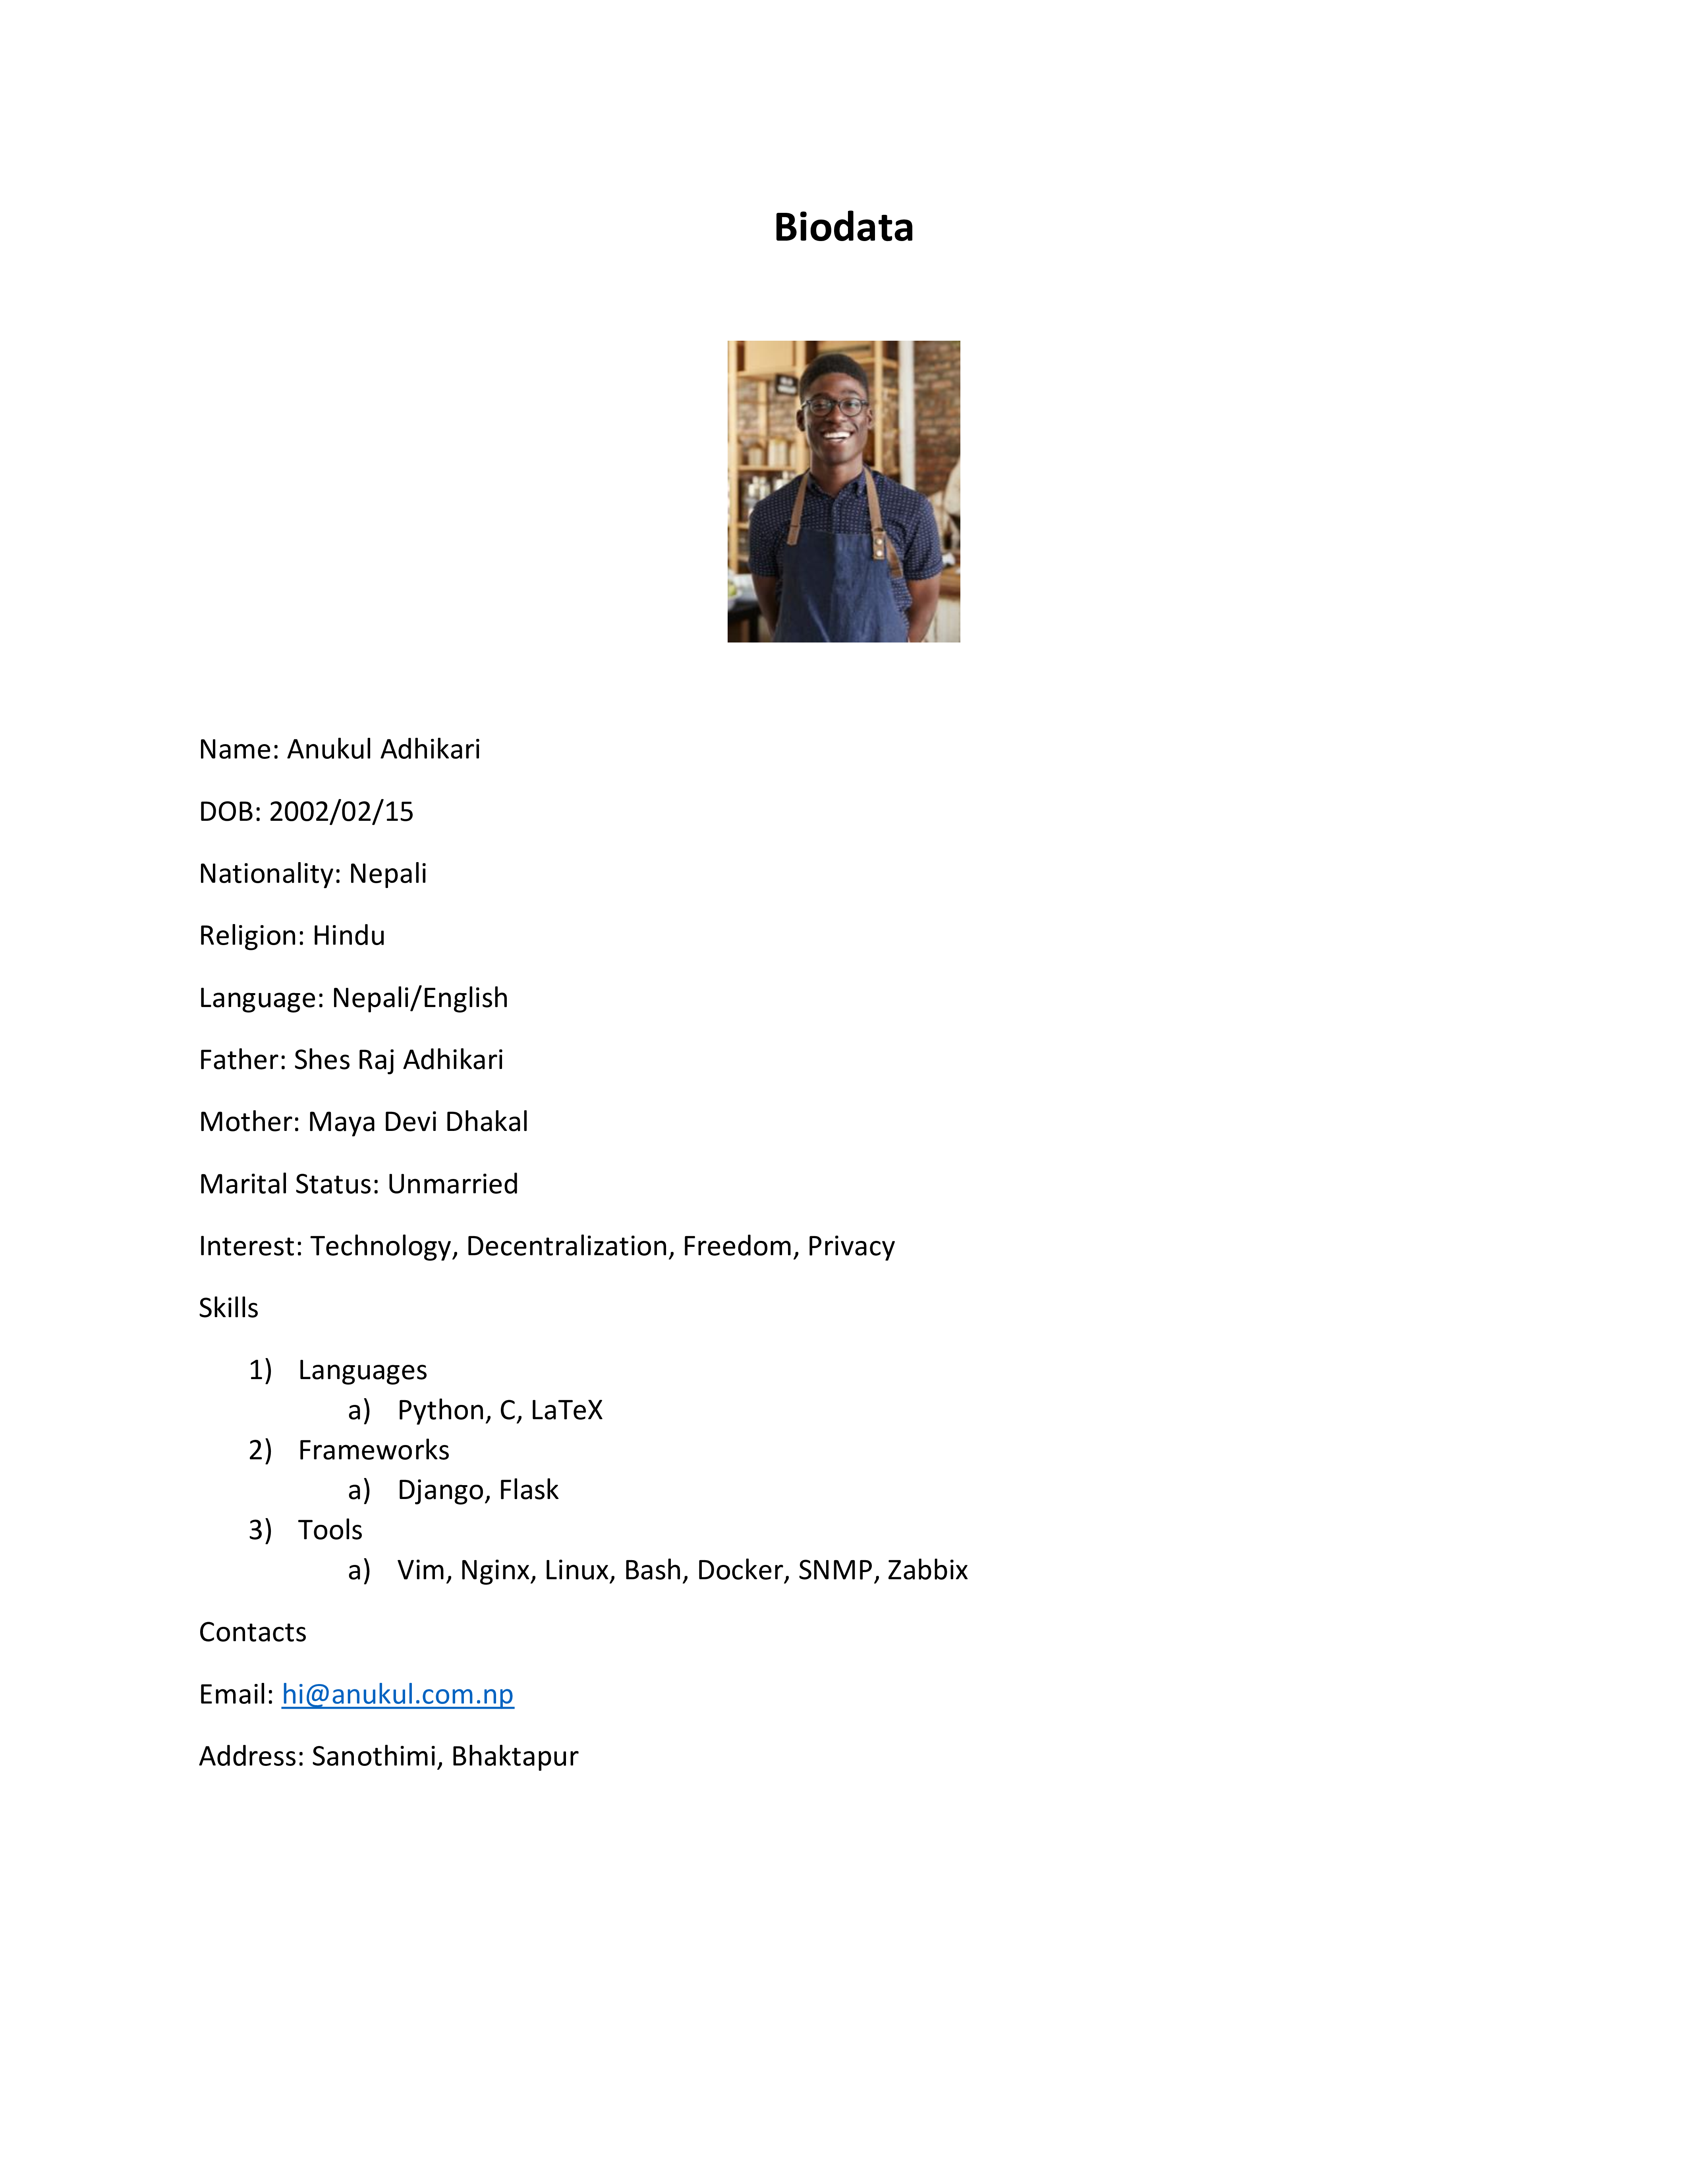
\includegraphics[width=1.5\textwidth]{./scrot/biography.png}
\pagebreak


\subsection{Identity Card}
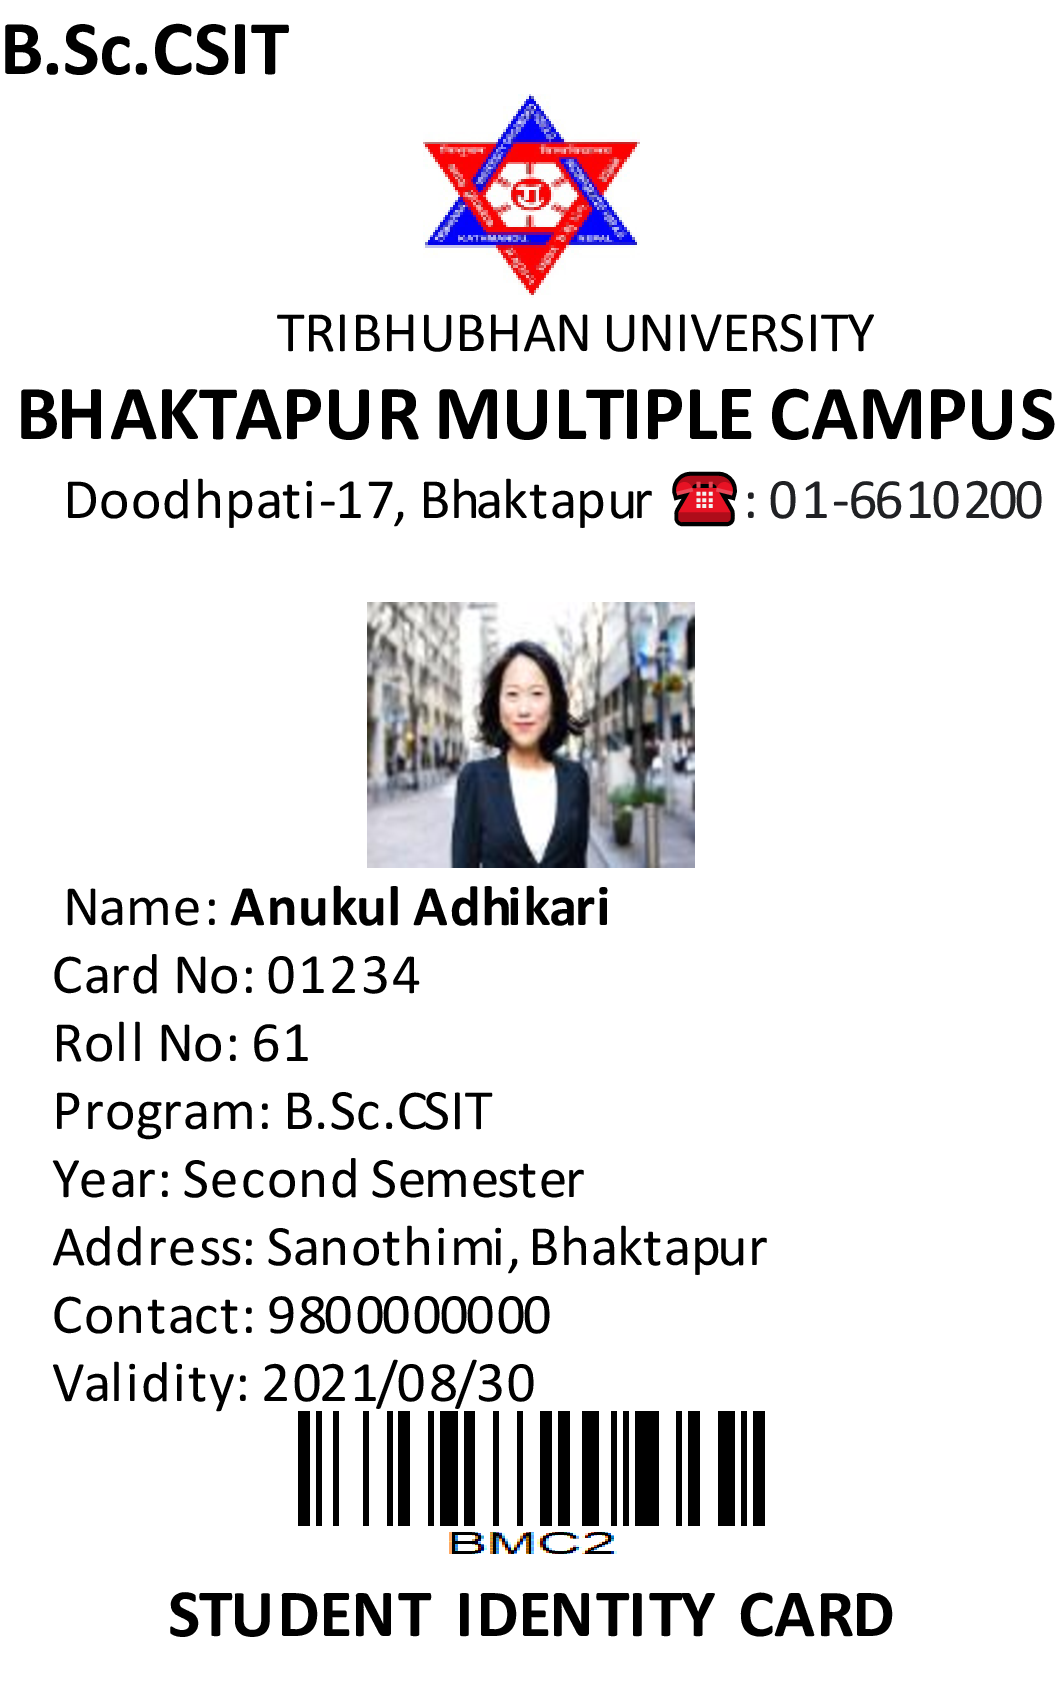
\includegraphics[width=1\textwidth]{./scrot/id-card.png}
\pagebreak

\subsection{Introduction to IPv6}
Internet Protocol version 6 is the next addressing system for Internet-connected devices. The explosive growth of the Internet has exceeded the capacity of the 30-year-old standard, known as IPv4, to handle all the network tools, websites, cell phones, and other devices that need unique addresses out in the World Wide Web. IPv4 has been a very successful standard with impressive durability. Not much else on the Internet has lasted 30 years unchanged, so they must have gotten a few things right when they designed it. However, the massive growth in the number and types of devices that use an Internet address has finally made a change necessary. IPv6 is that change. IPv4 uses a 32-bit address, usually expressed as a group of four address numbers from 0 to 255, which made around 4.3 billion addresses available. The vast majority of these addresses have already been assigned to Internet service providers. IPv6’s 128-bit address provides for many times that amount of addresses. To be exact, IPv6 will supply 2128 or 340 undecillion or 3.4x1038 addresses!

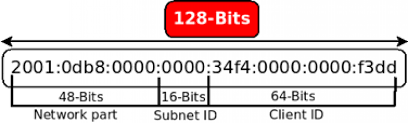
\includegraphics[width=1\textwidth]{./scrot/ipv6.png}
\pagebreak

\subsection{Class Routine}
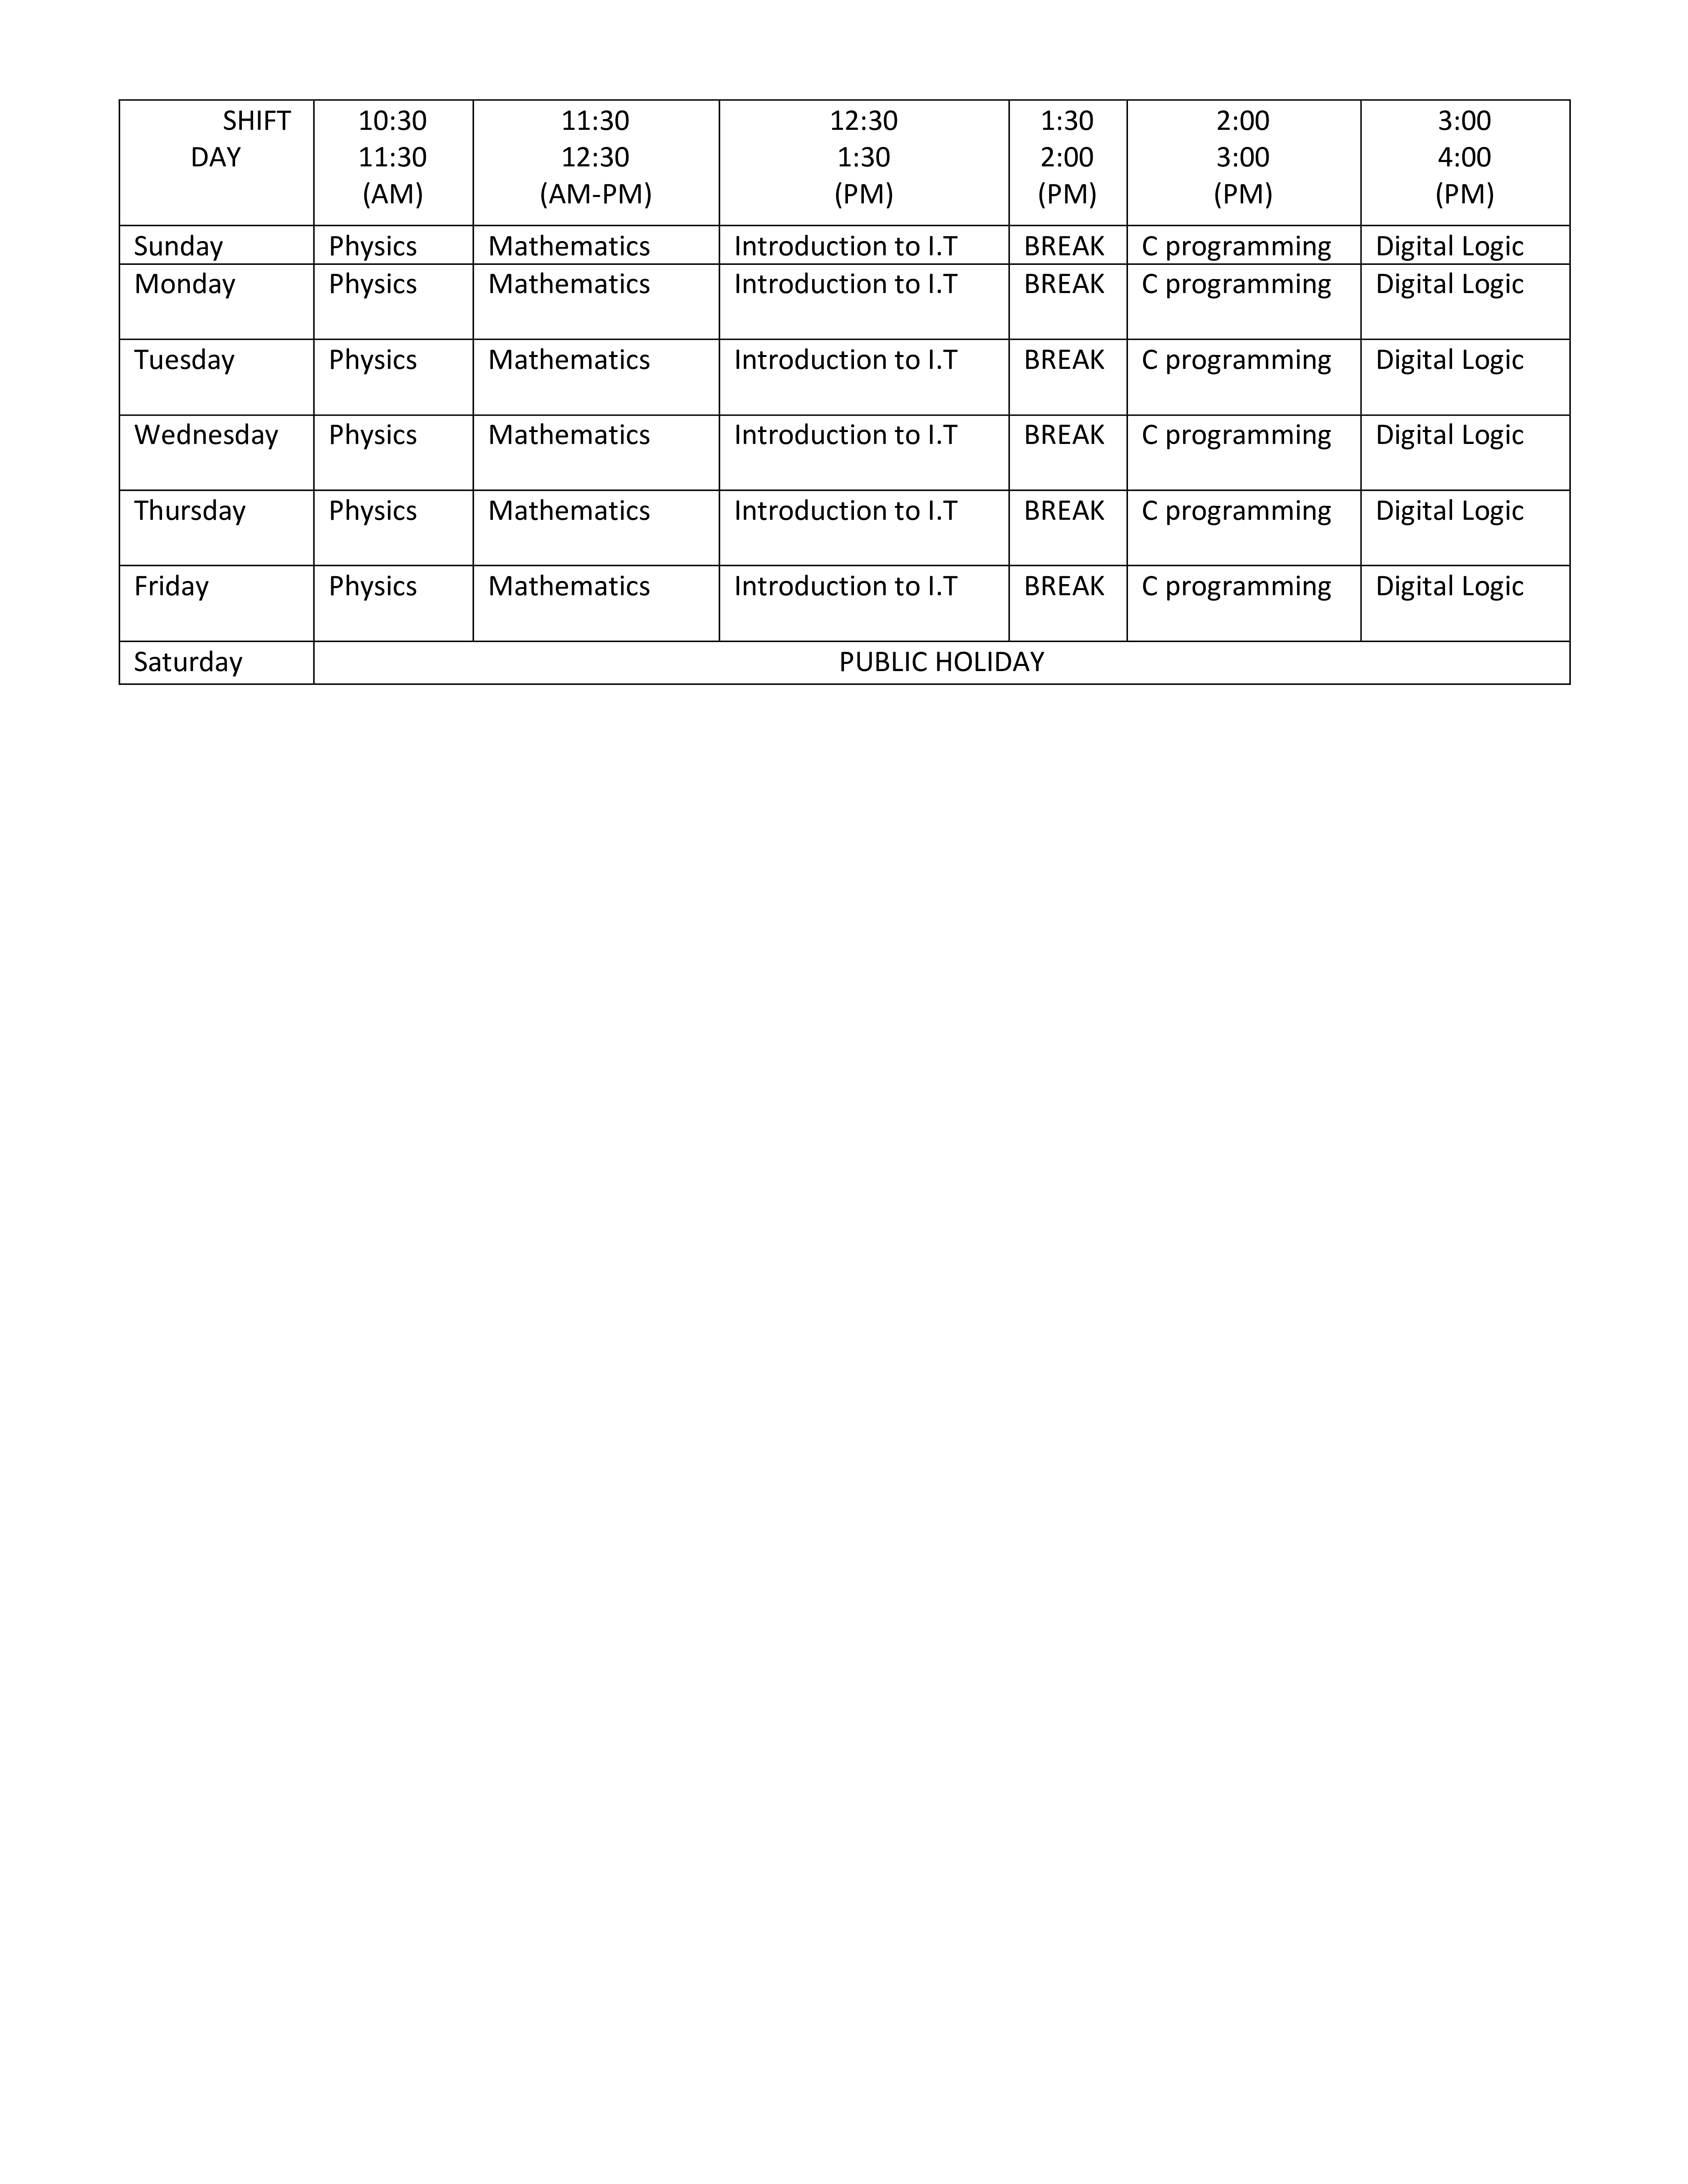
\includegraphics[width=1.2\textwidth]{./scrot/routine.png}
\pagebreak

\subsection{Mark Sheet of SEE}
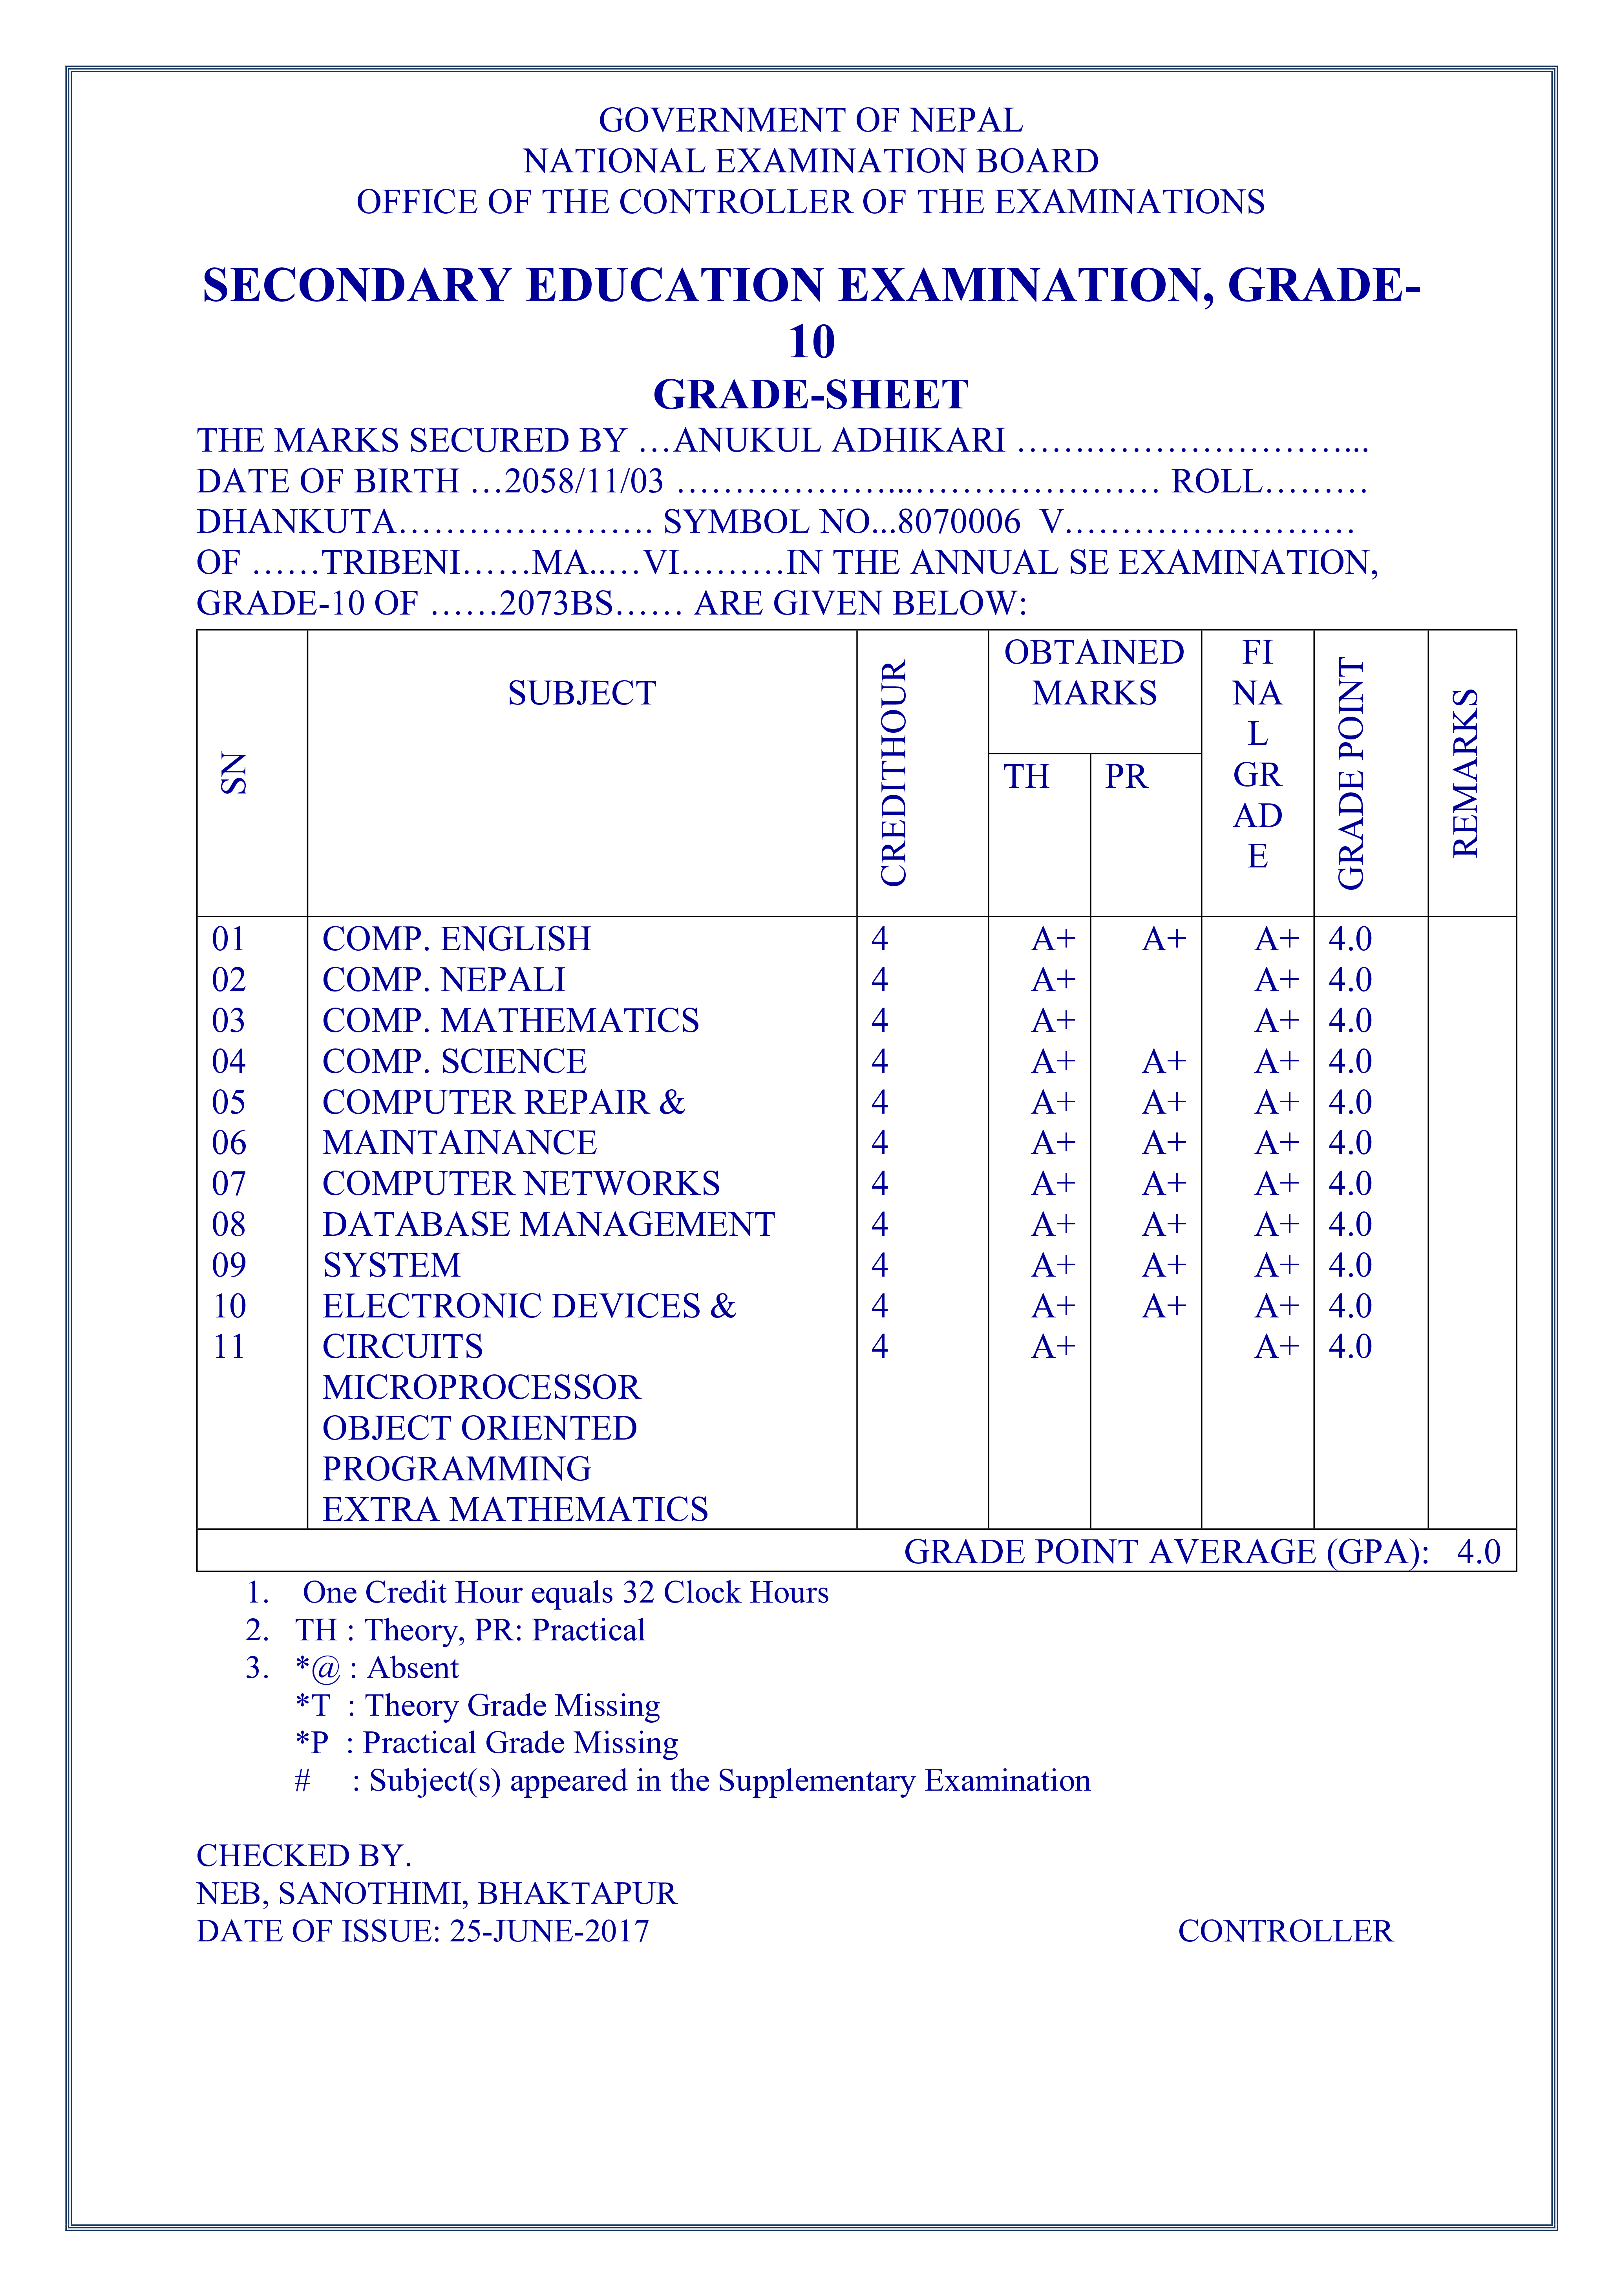
\includegraphics[width=1.2\textwidth]{./scrot/see.png}
\pagebreak

\section{Project Work on Spreadsheet}
\subsection{Find out Bonus, TAX,P.F. and net salary.}
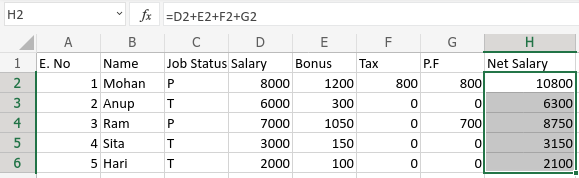
\includegraphics[width=1\textwidth]{./scrot/spreadsheet-1.png}

\subsection{Find out Total, Percentage, Division and Result.}
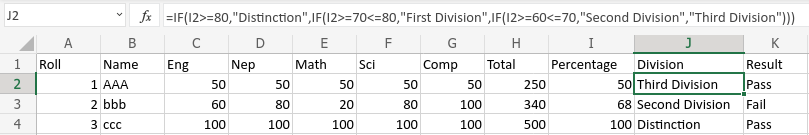
\includegraphics[width=1\textwidth]{./scrot/spreadsheet-2.png}

\subsection{Create a line chart.}
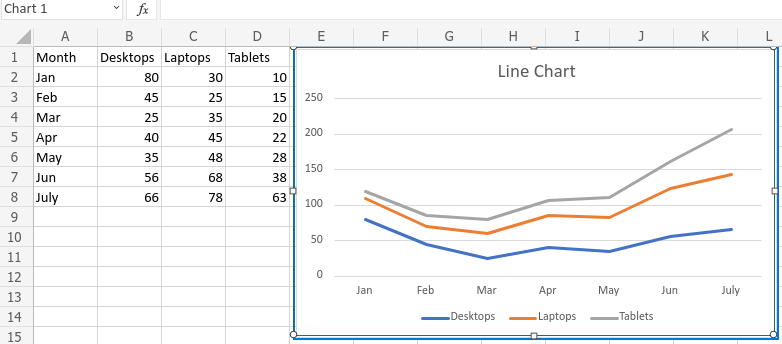
\includegraphics[width=1\textwidth]{./scrot/spreadsheet-3.png}

\subsection{Create a bar graph.}
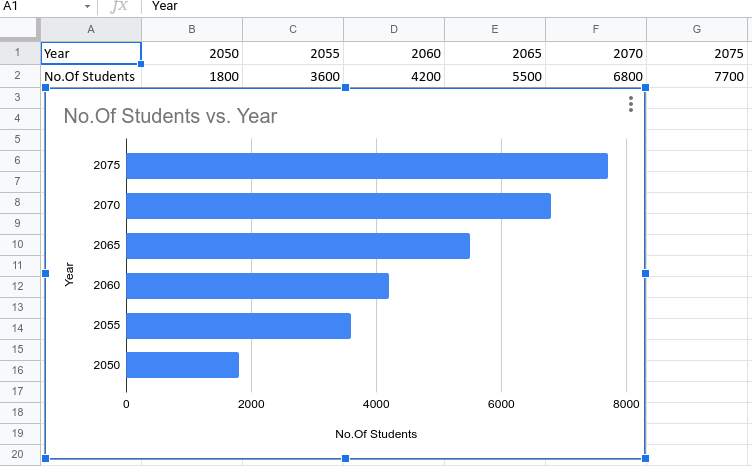
\includegraphics[width=1\textwidth]{./scrot/spreadsheet-4.png}

\subsection{Design Pie Chart.}
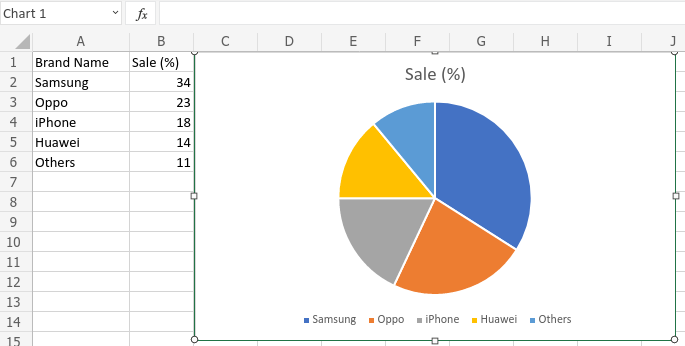
\includegraphics[width=1\textwidth]{./scrot/spreadsheet-5.png}


\section{Project work on Presentation}


\subsection{Input Devices}
\begin{center}
	
\includegraphics[width=0.7\linewidth]{./scrot/input-0.png}
	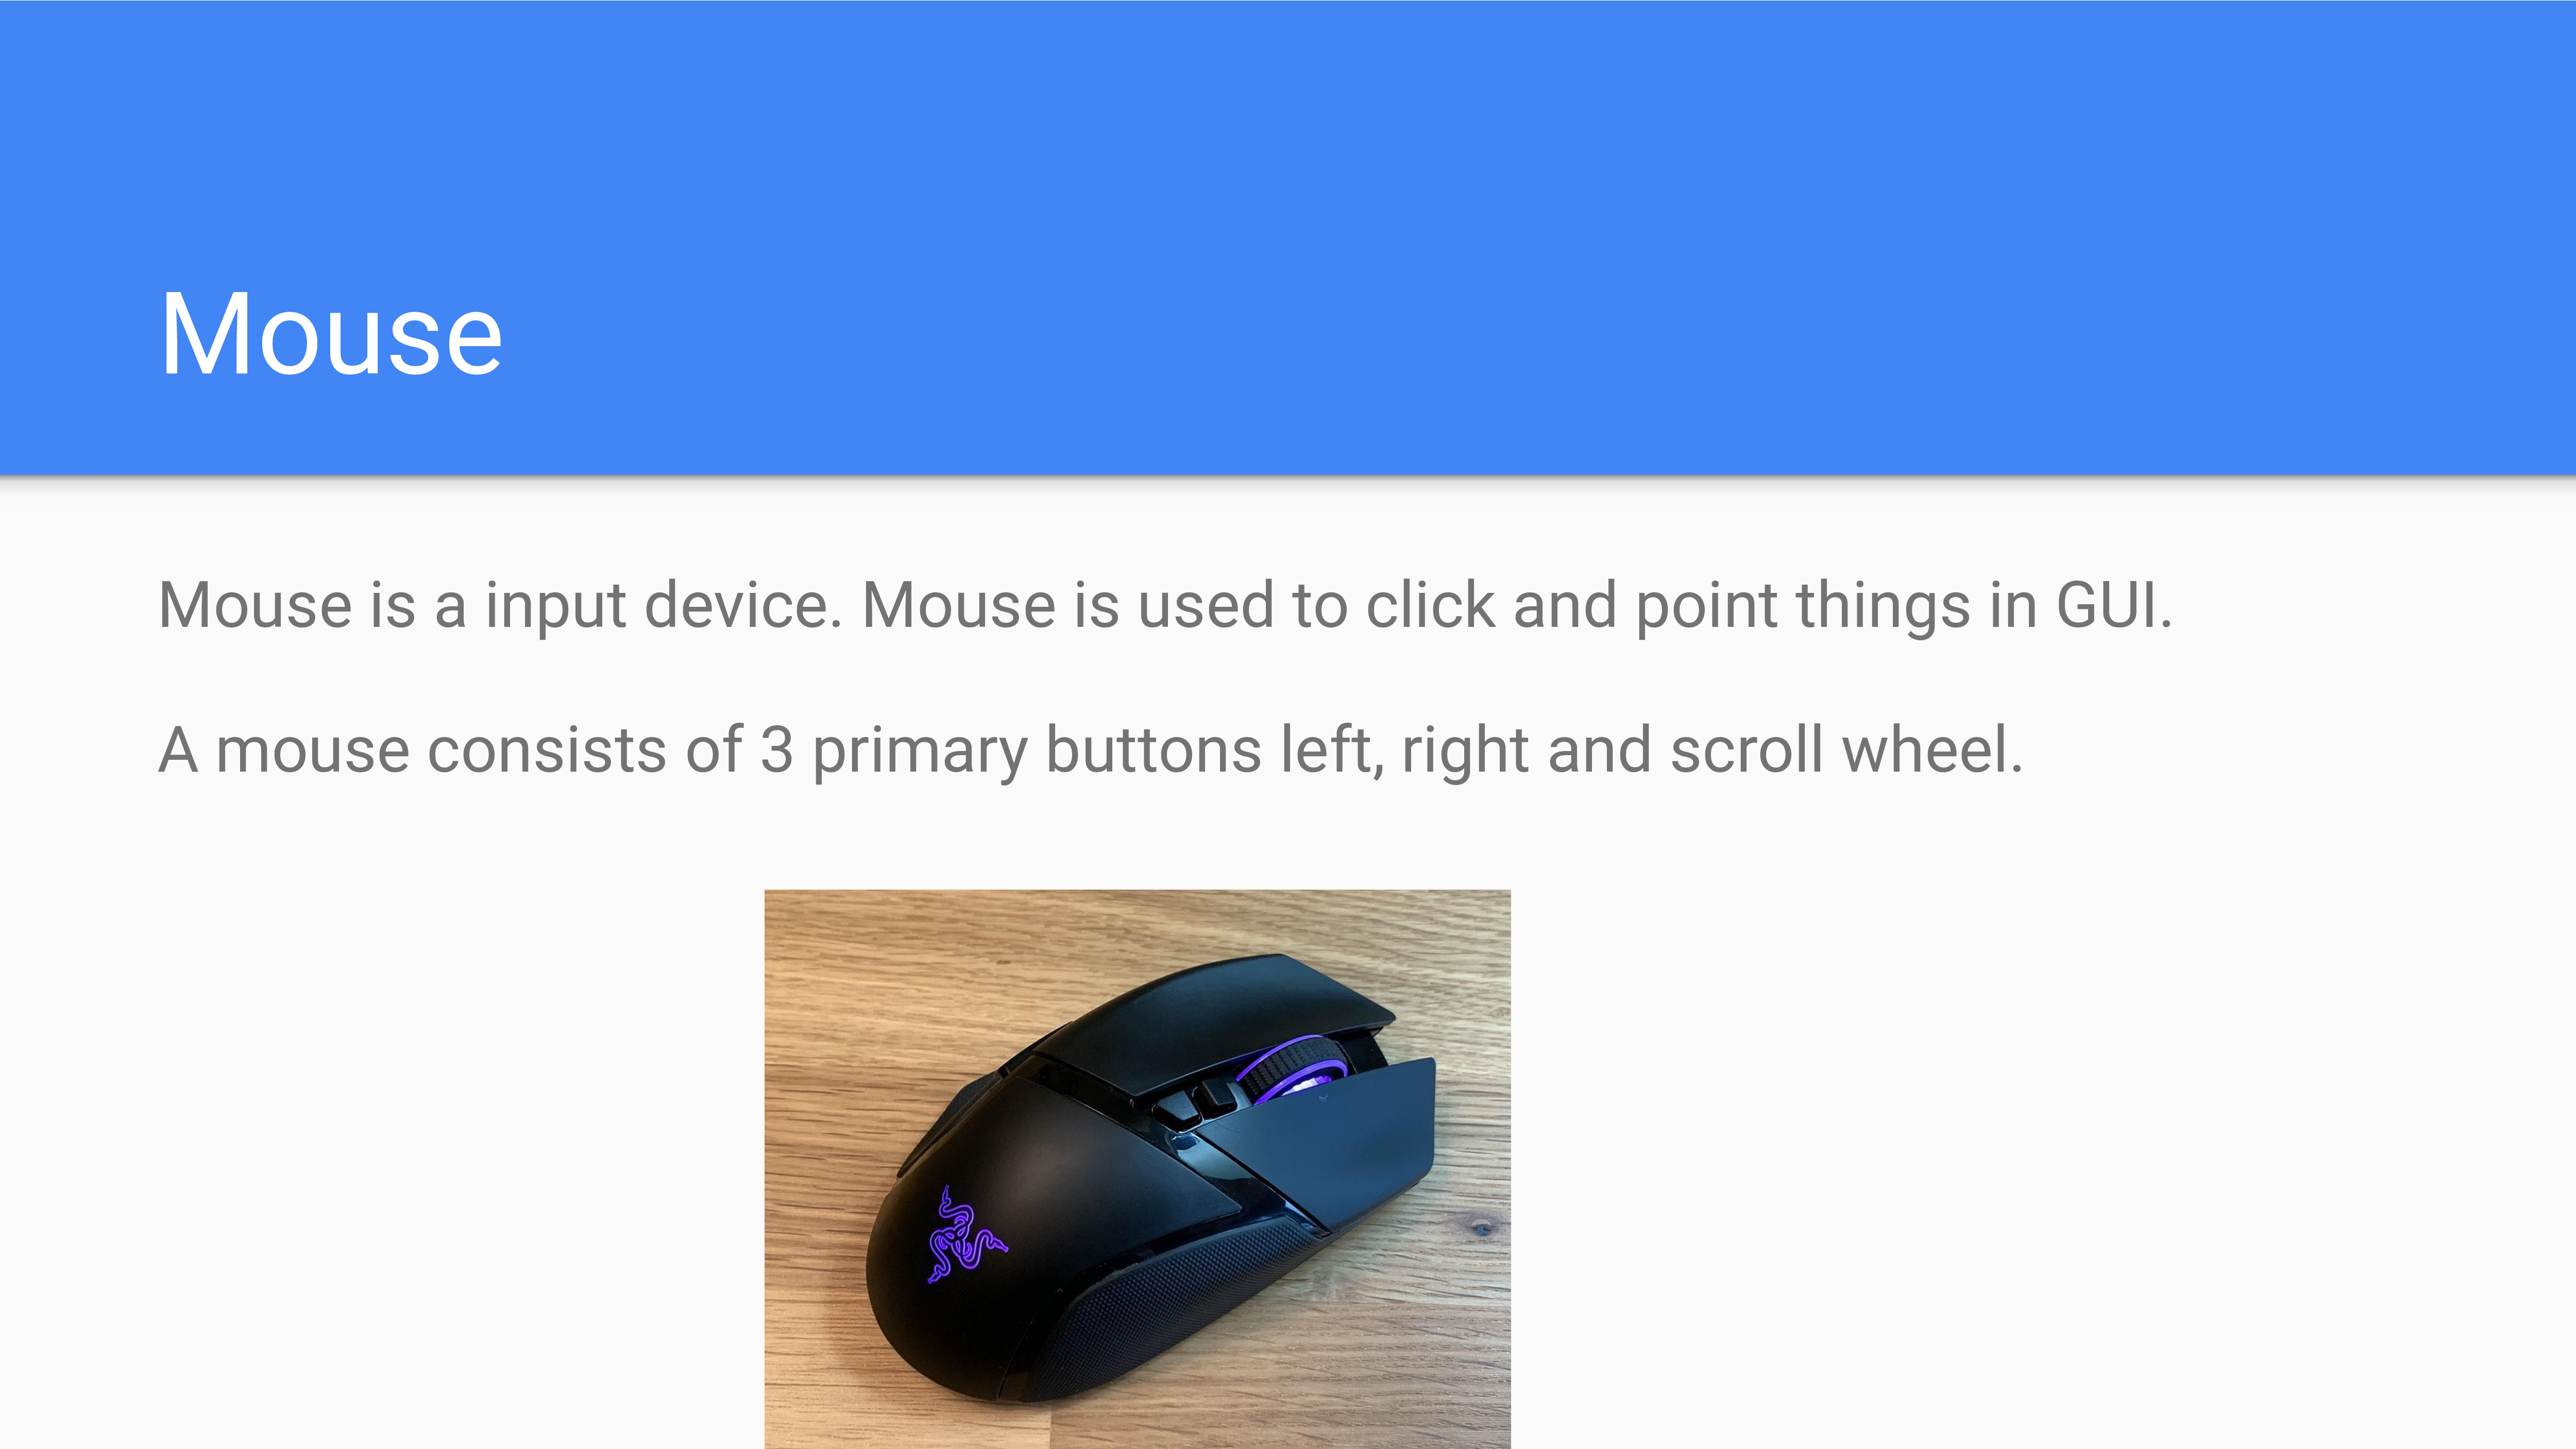
\includegraphics[width=0.7\linewidth]{./scrot/input-1.png}
	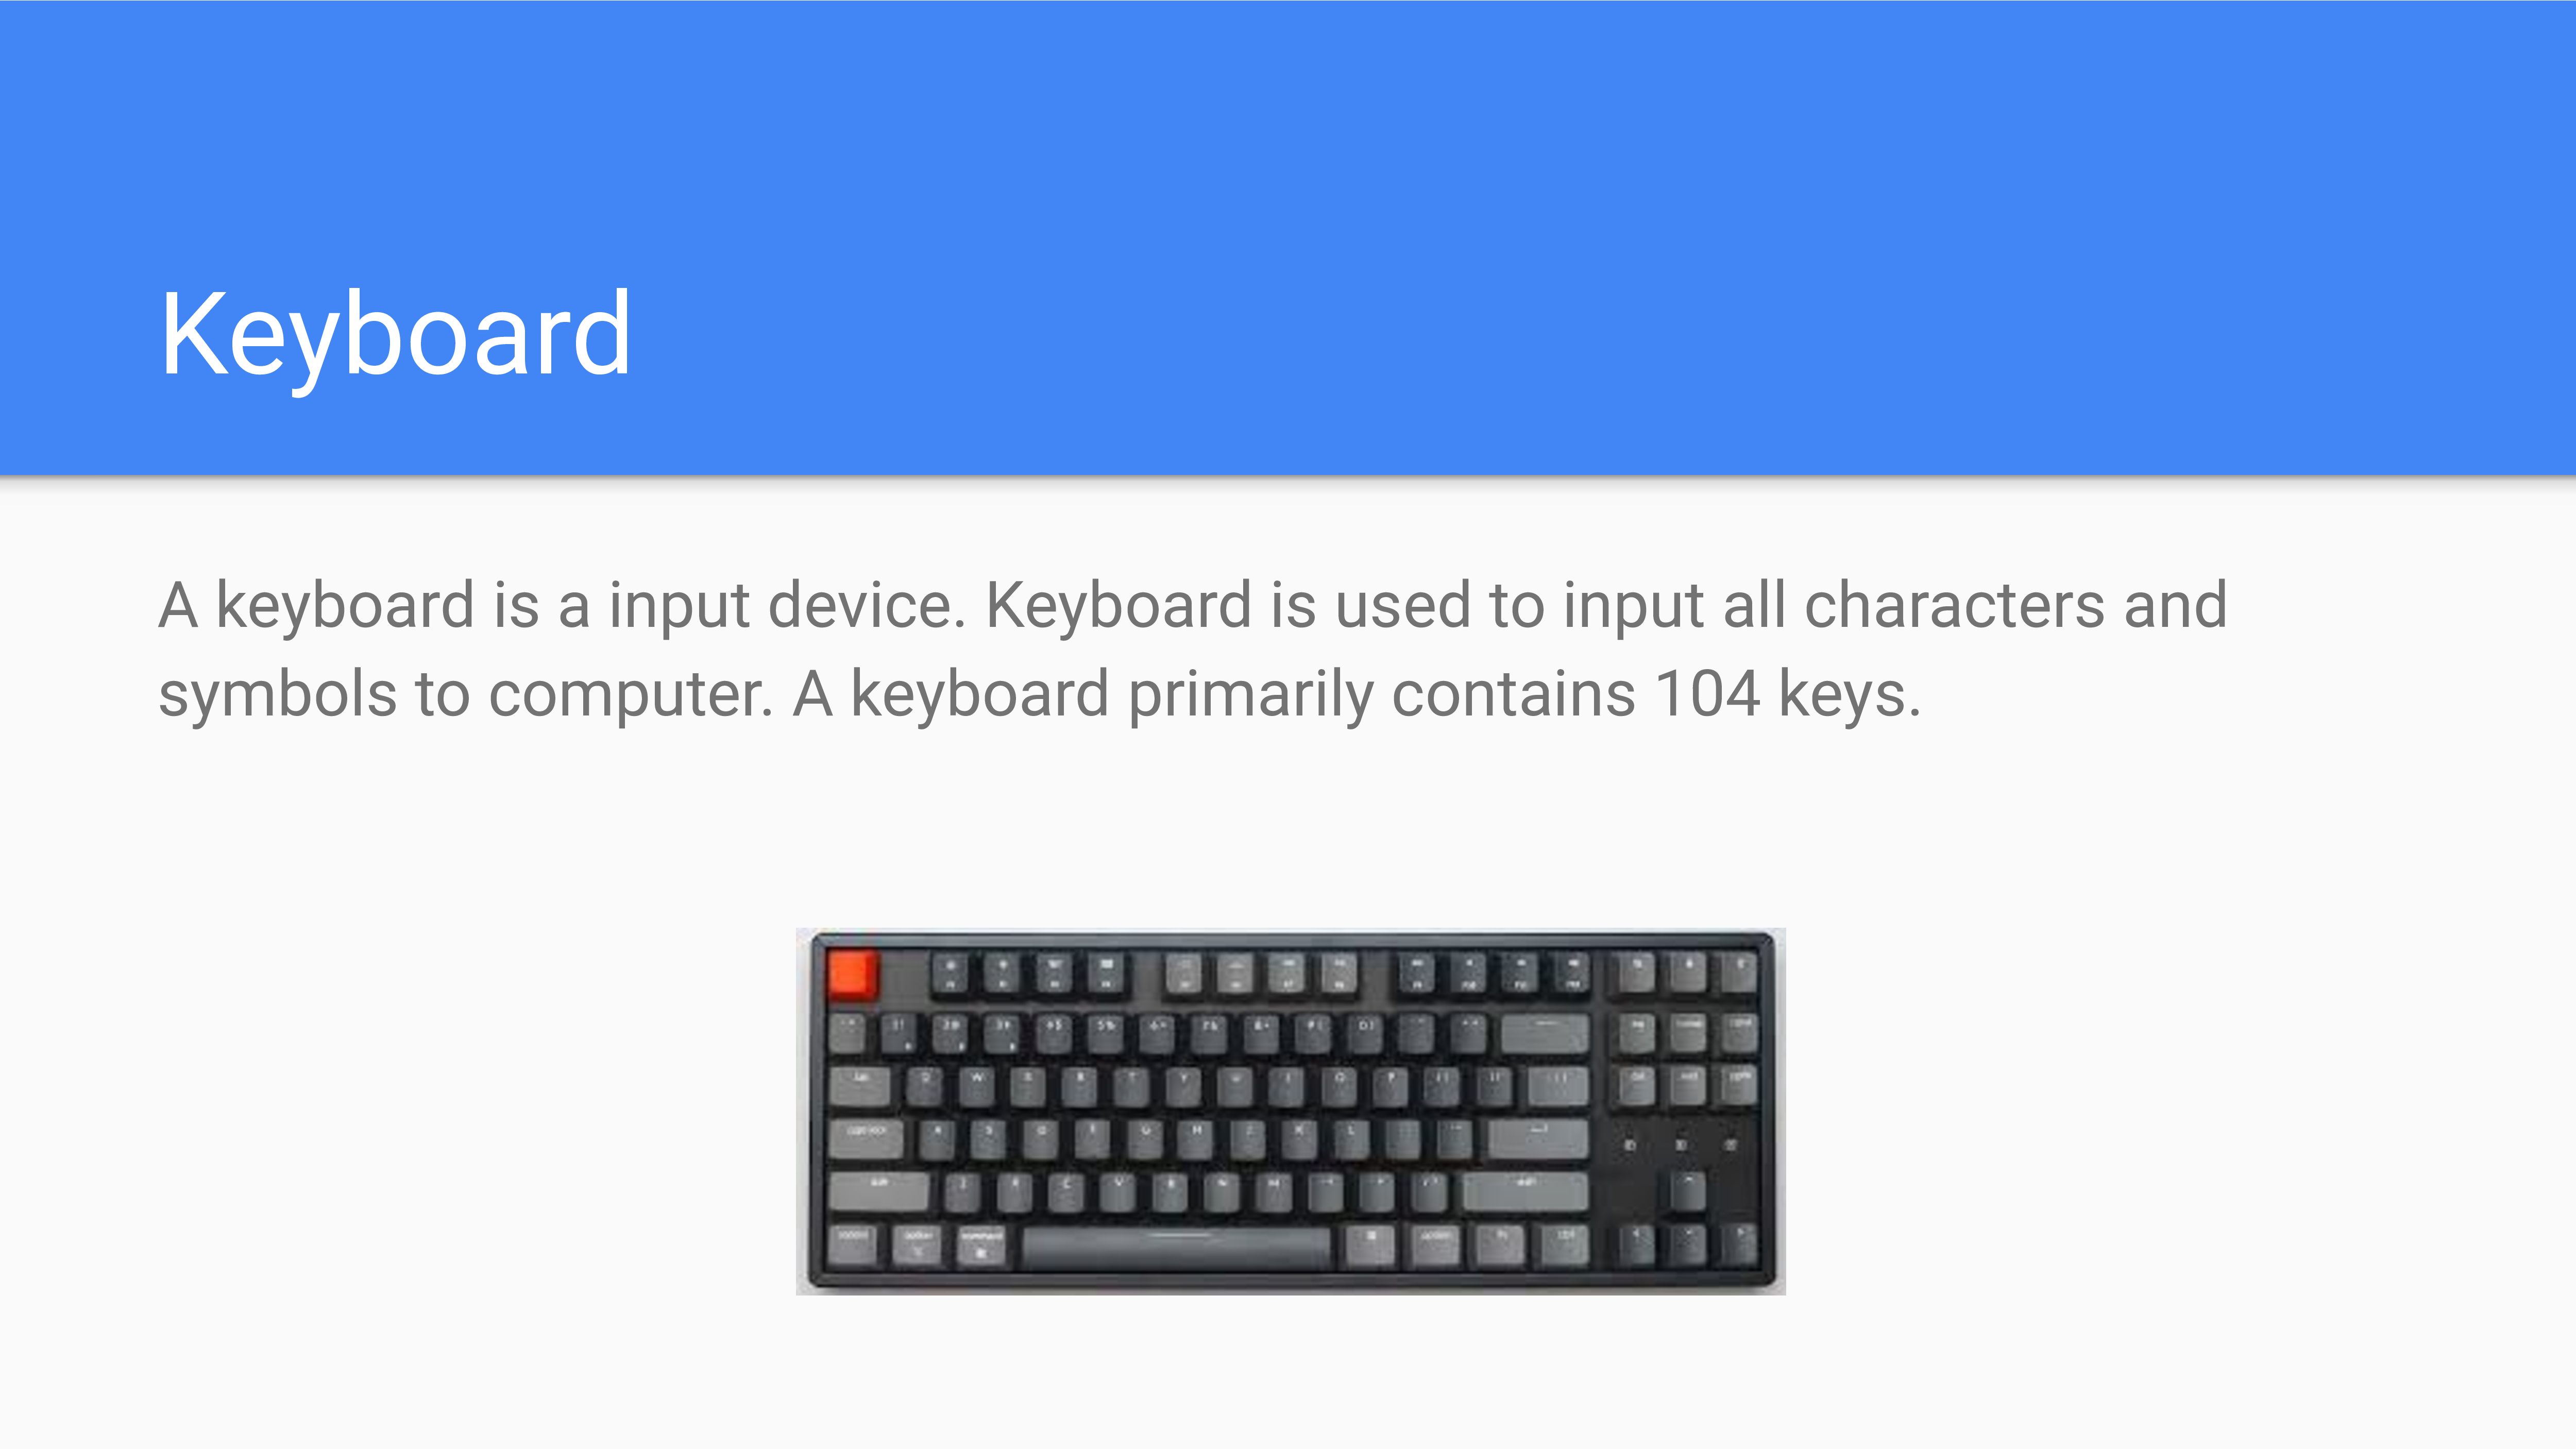
\includegraphics[width=0.7\linewidth]{./scrot/input-2.png}
	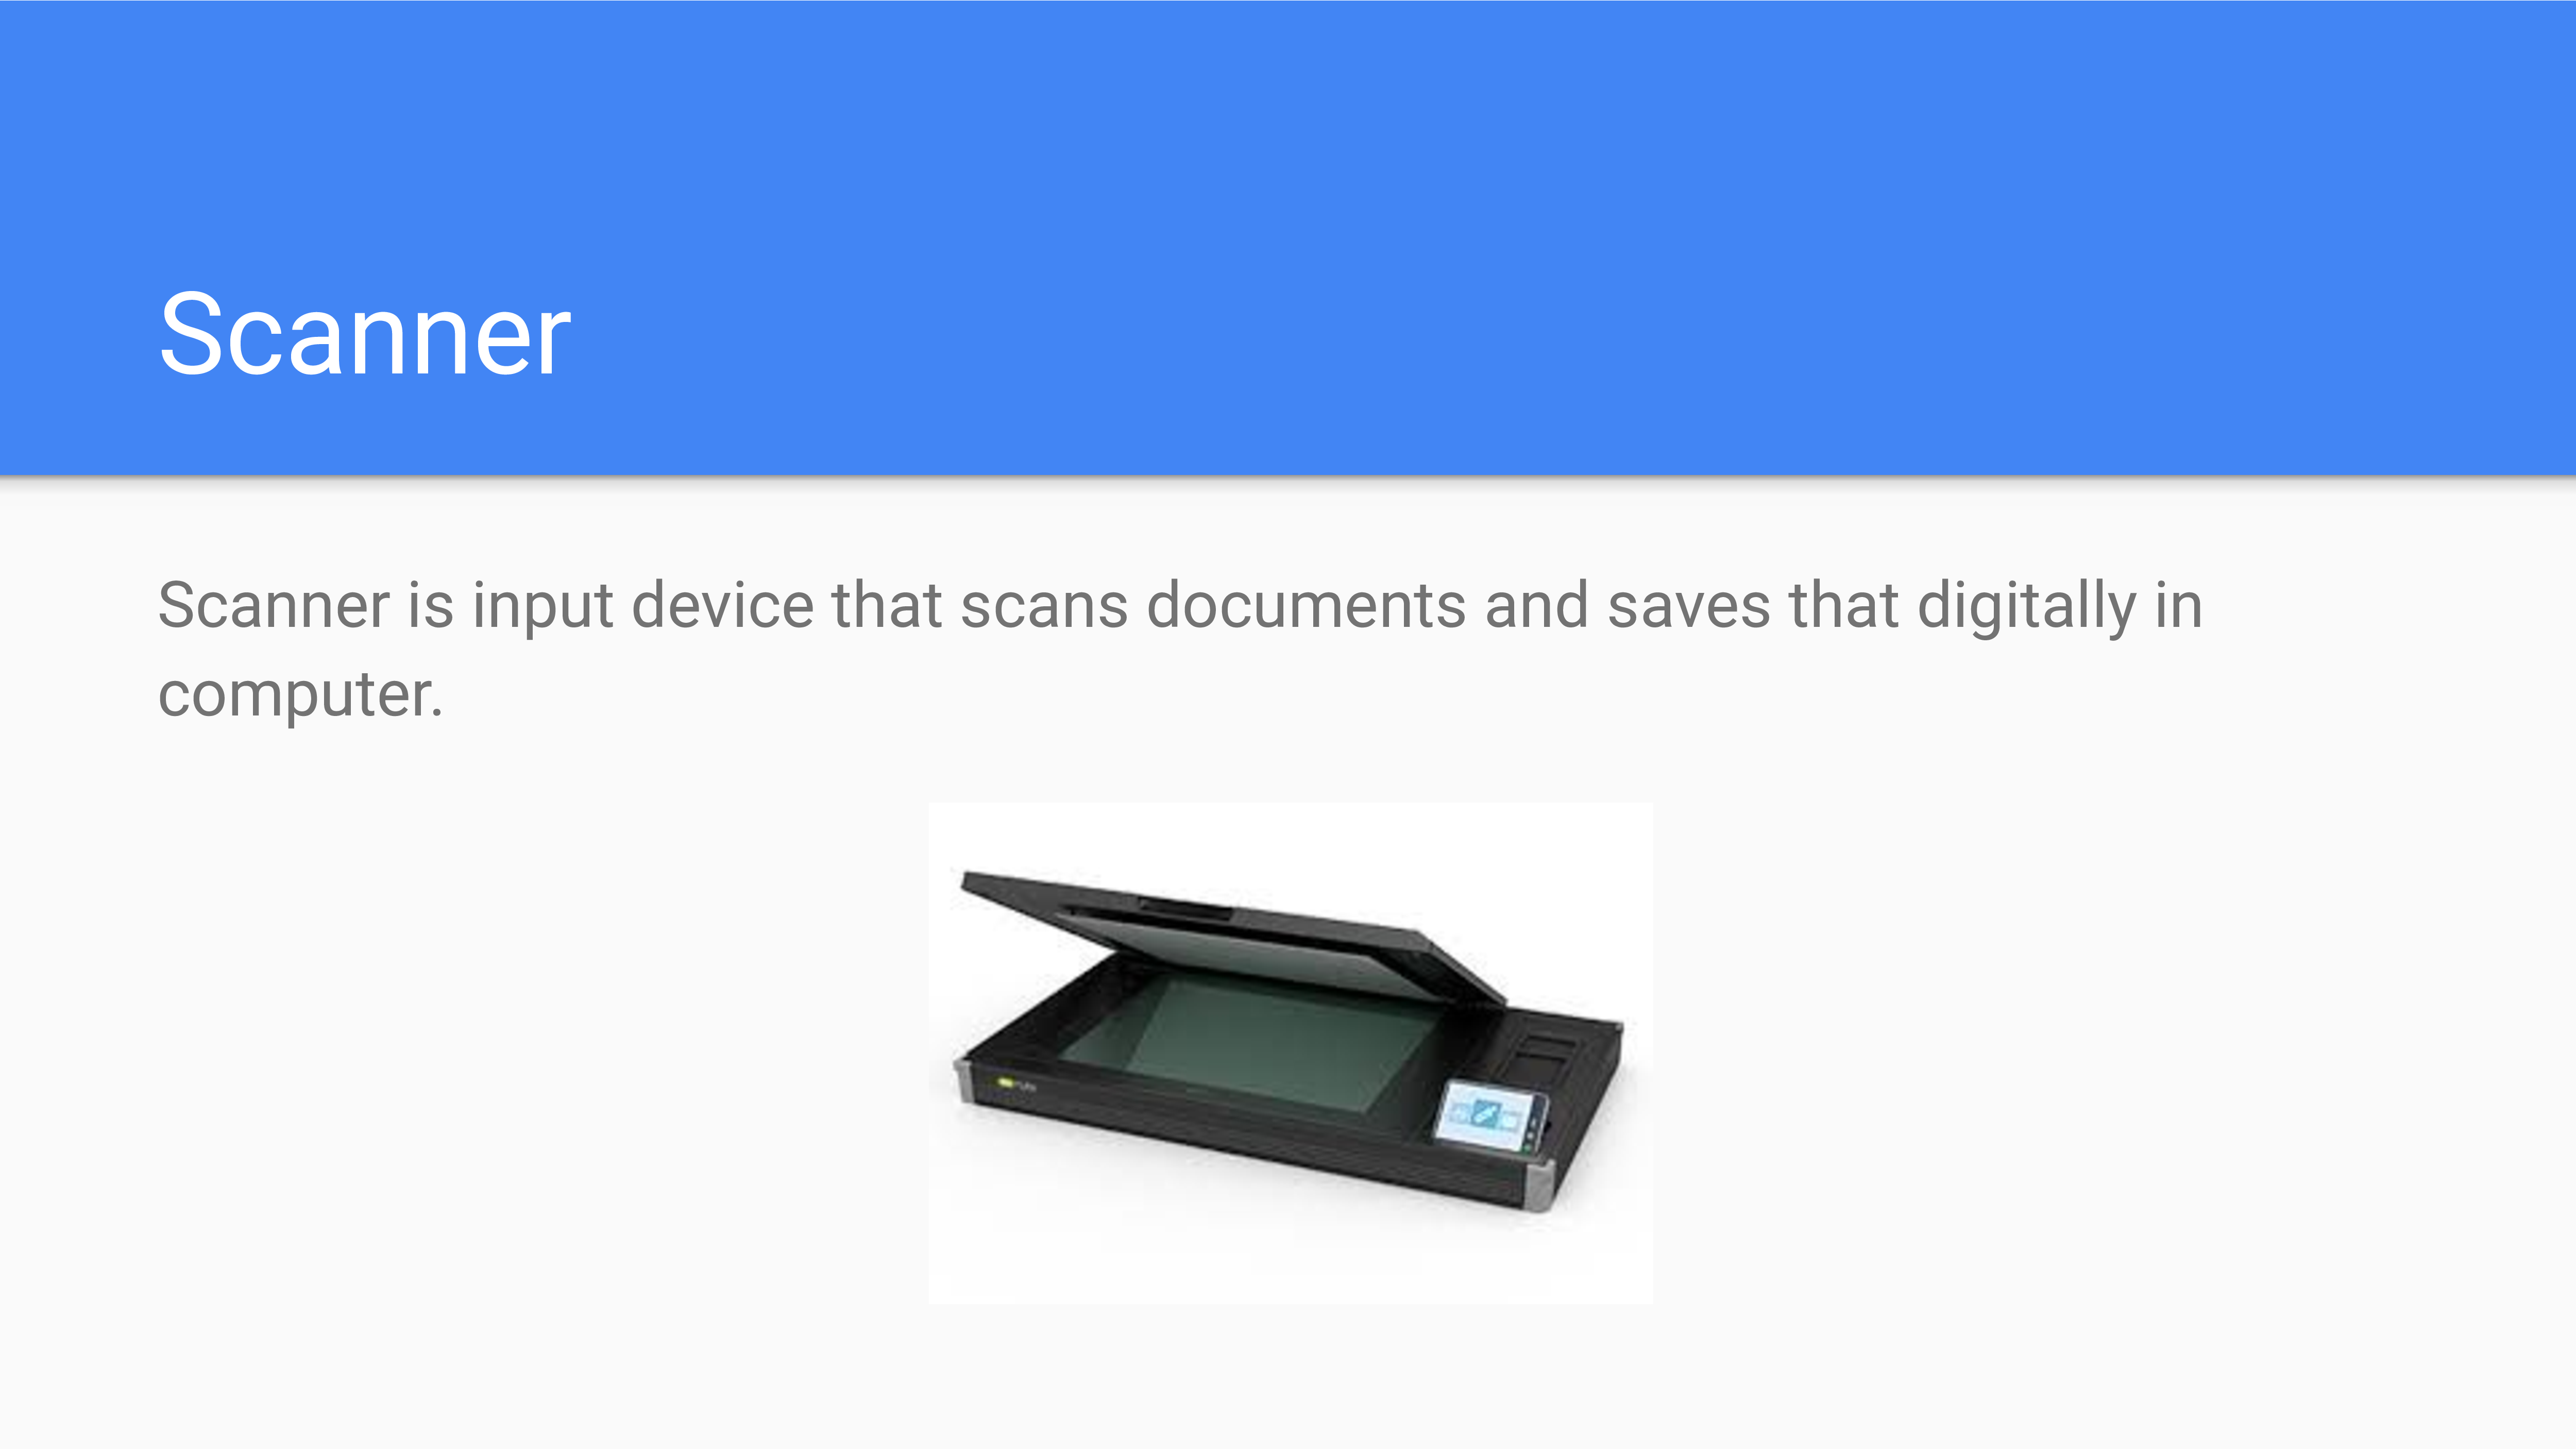
\includegraphics[width=0.7\linewidth]{./scrot/input-3.png}
\end{center}
\begin{center}
	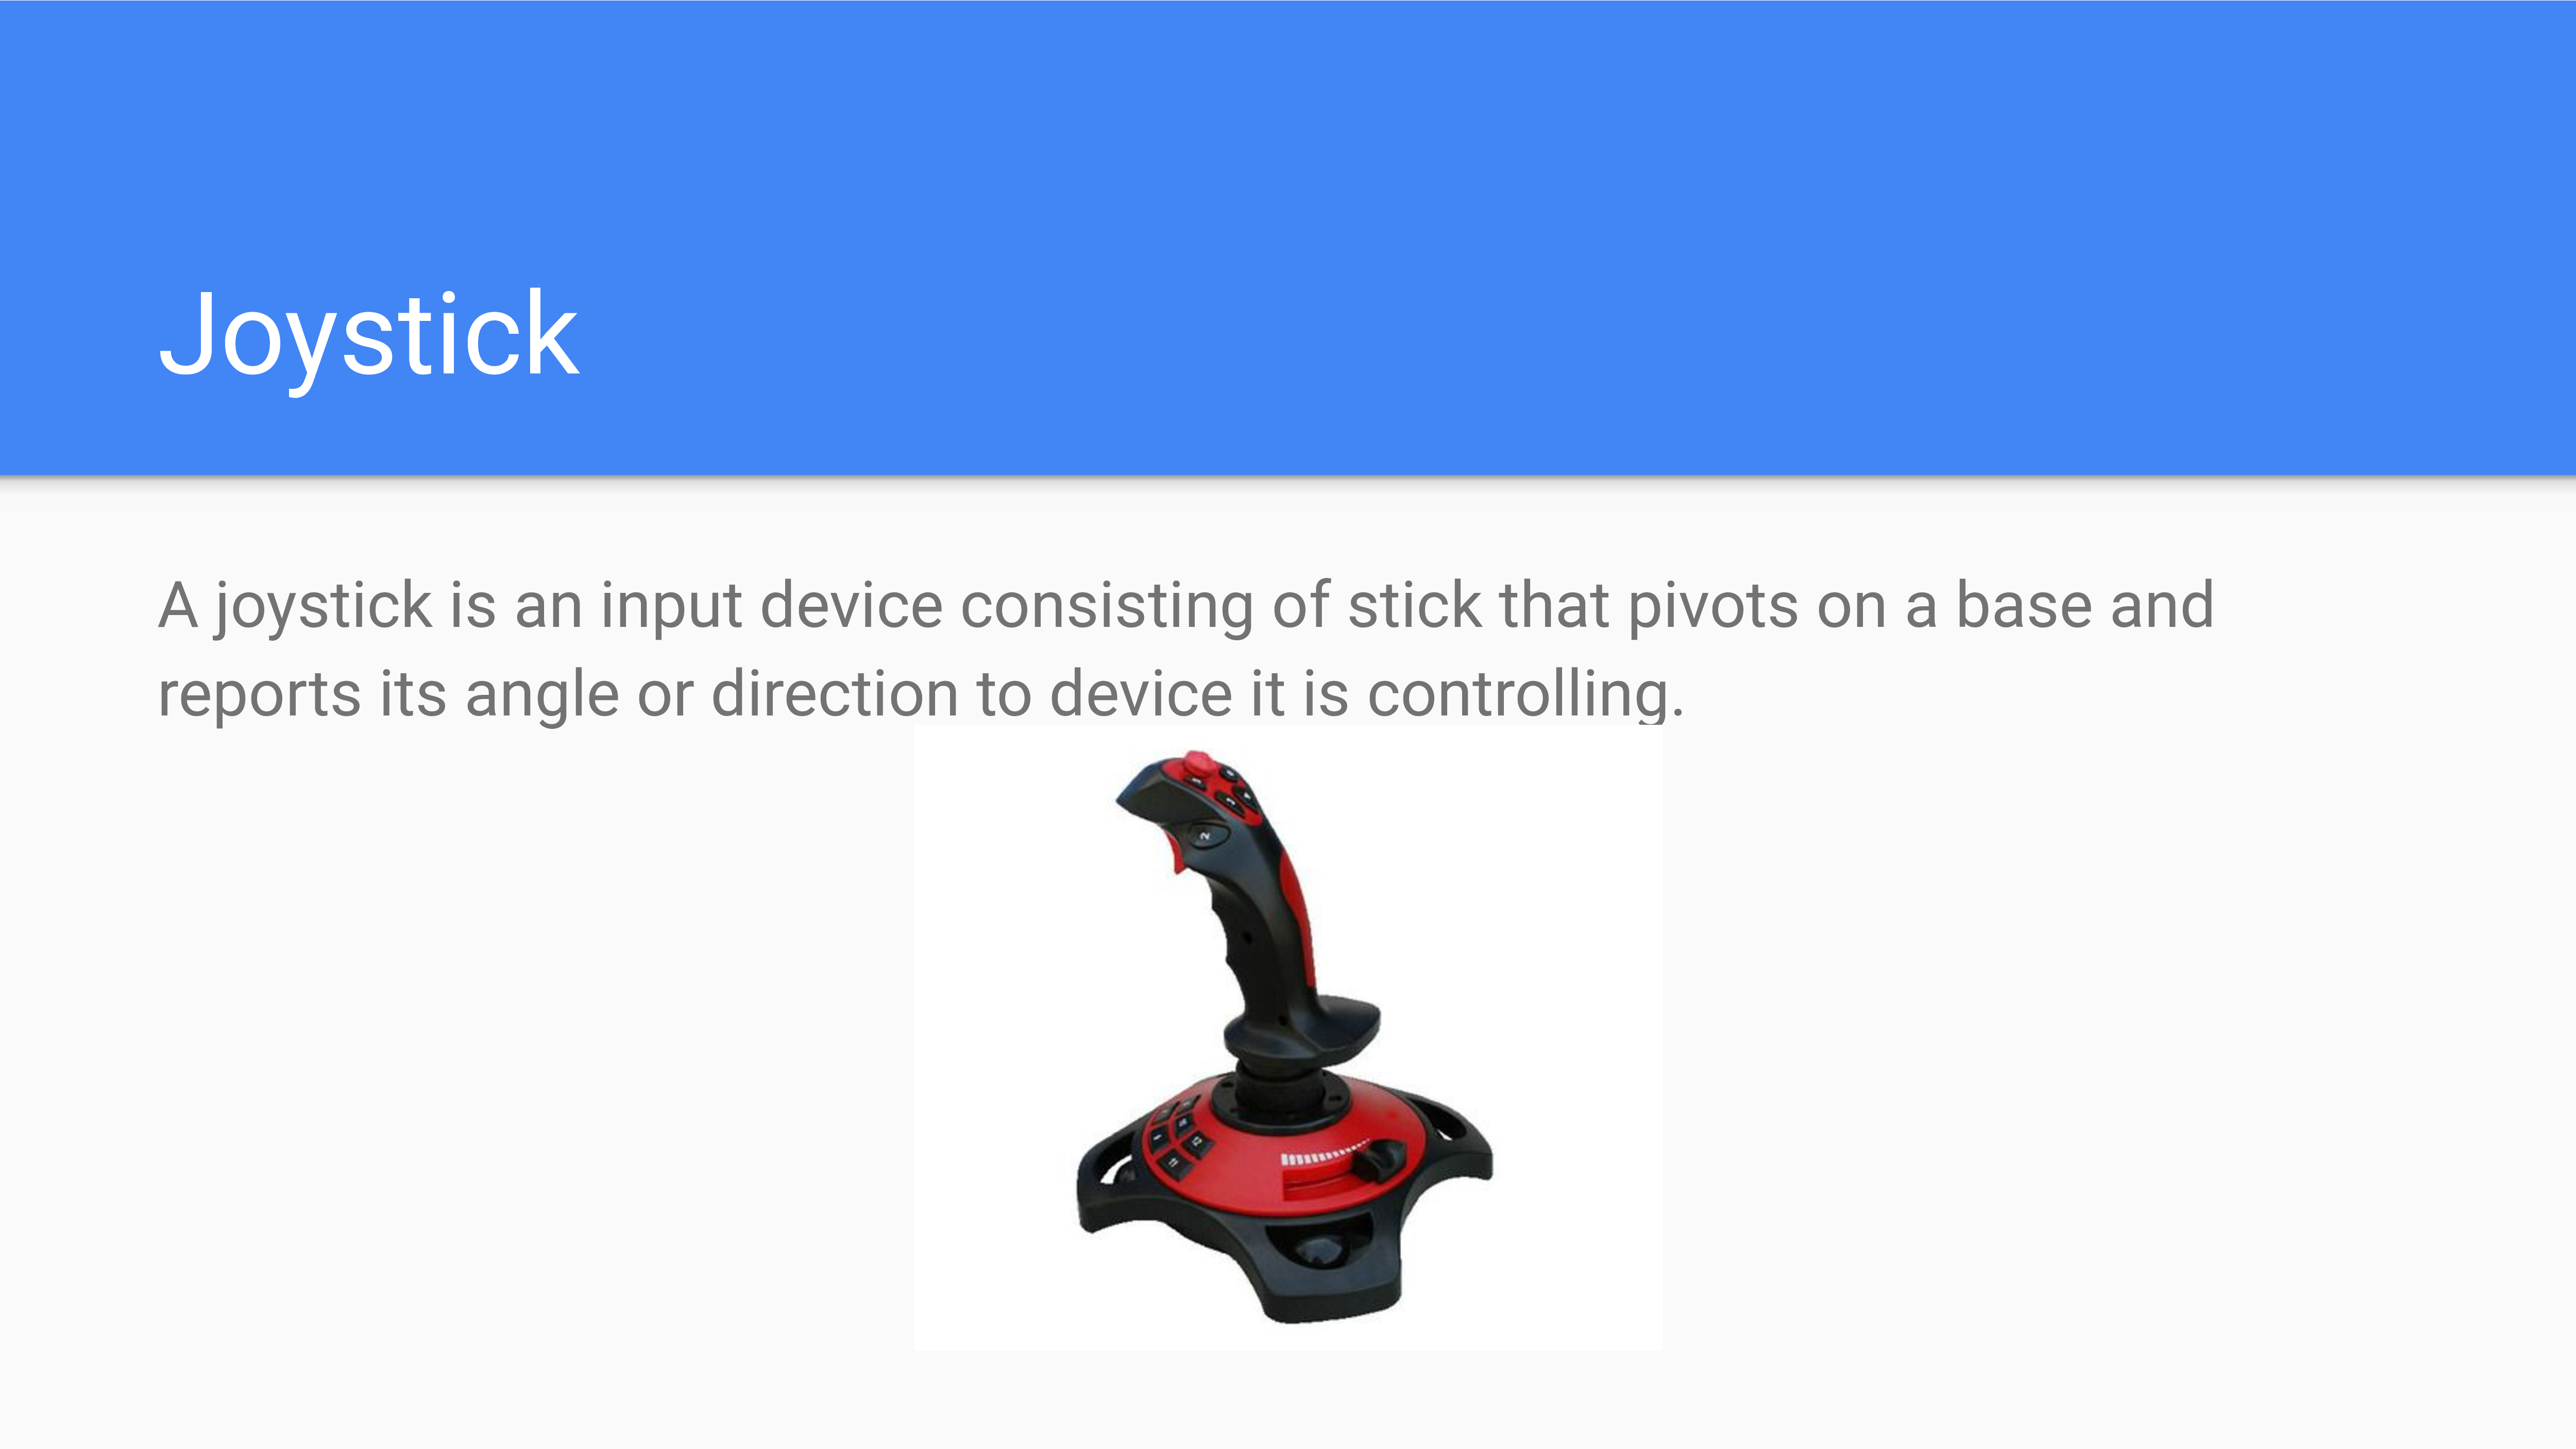
\includegraphics[width=0.7\linewidth]{./scrot/input-4.png}
	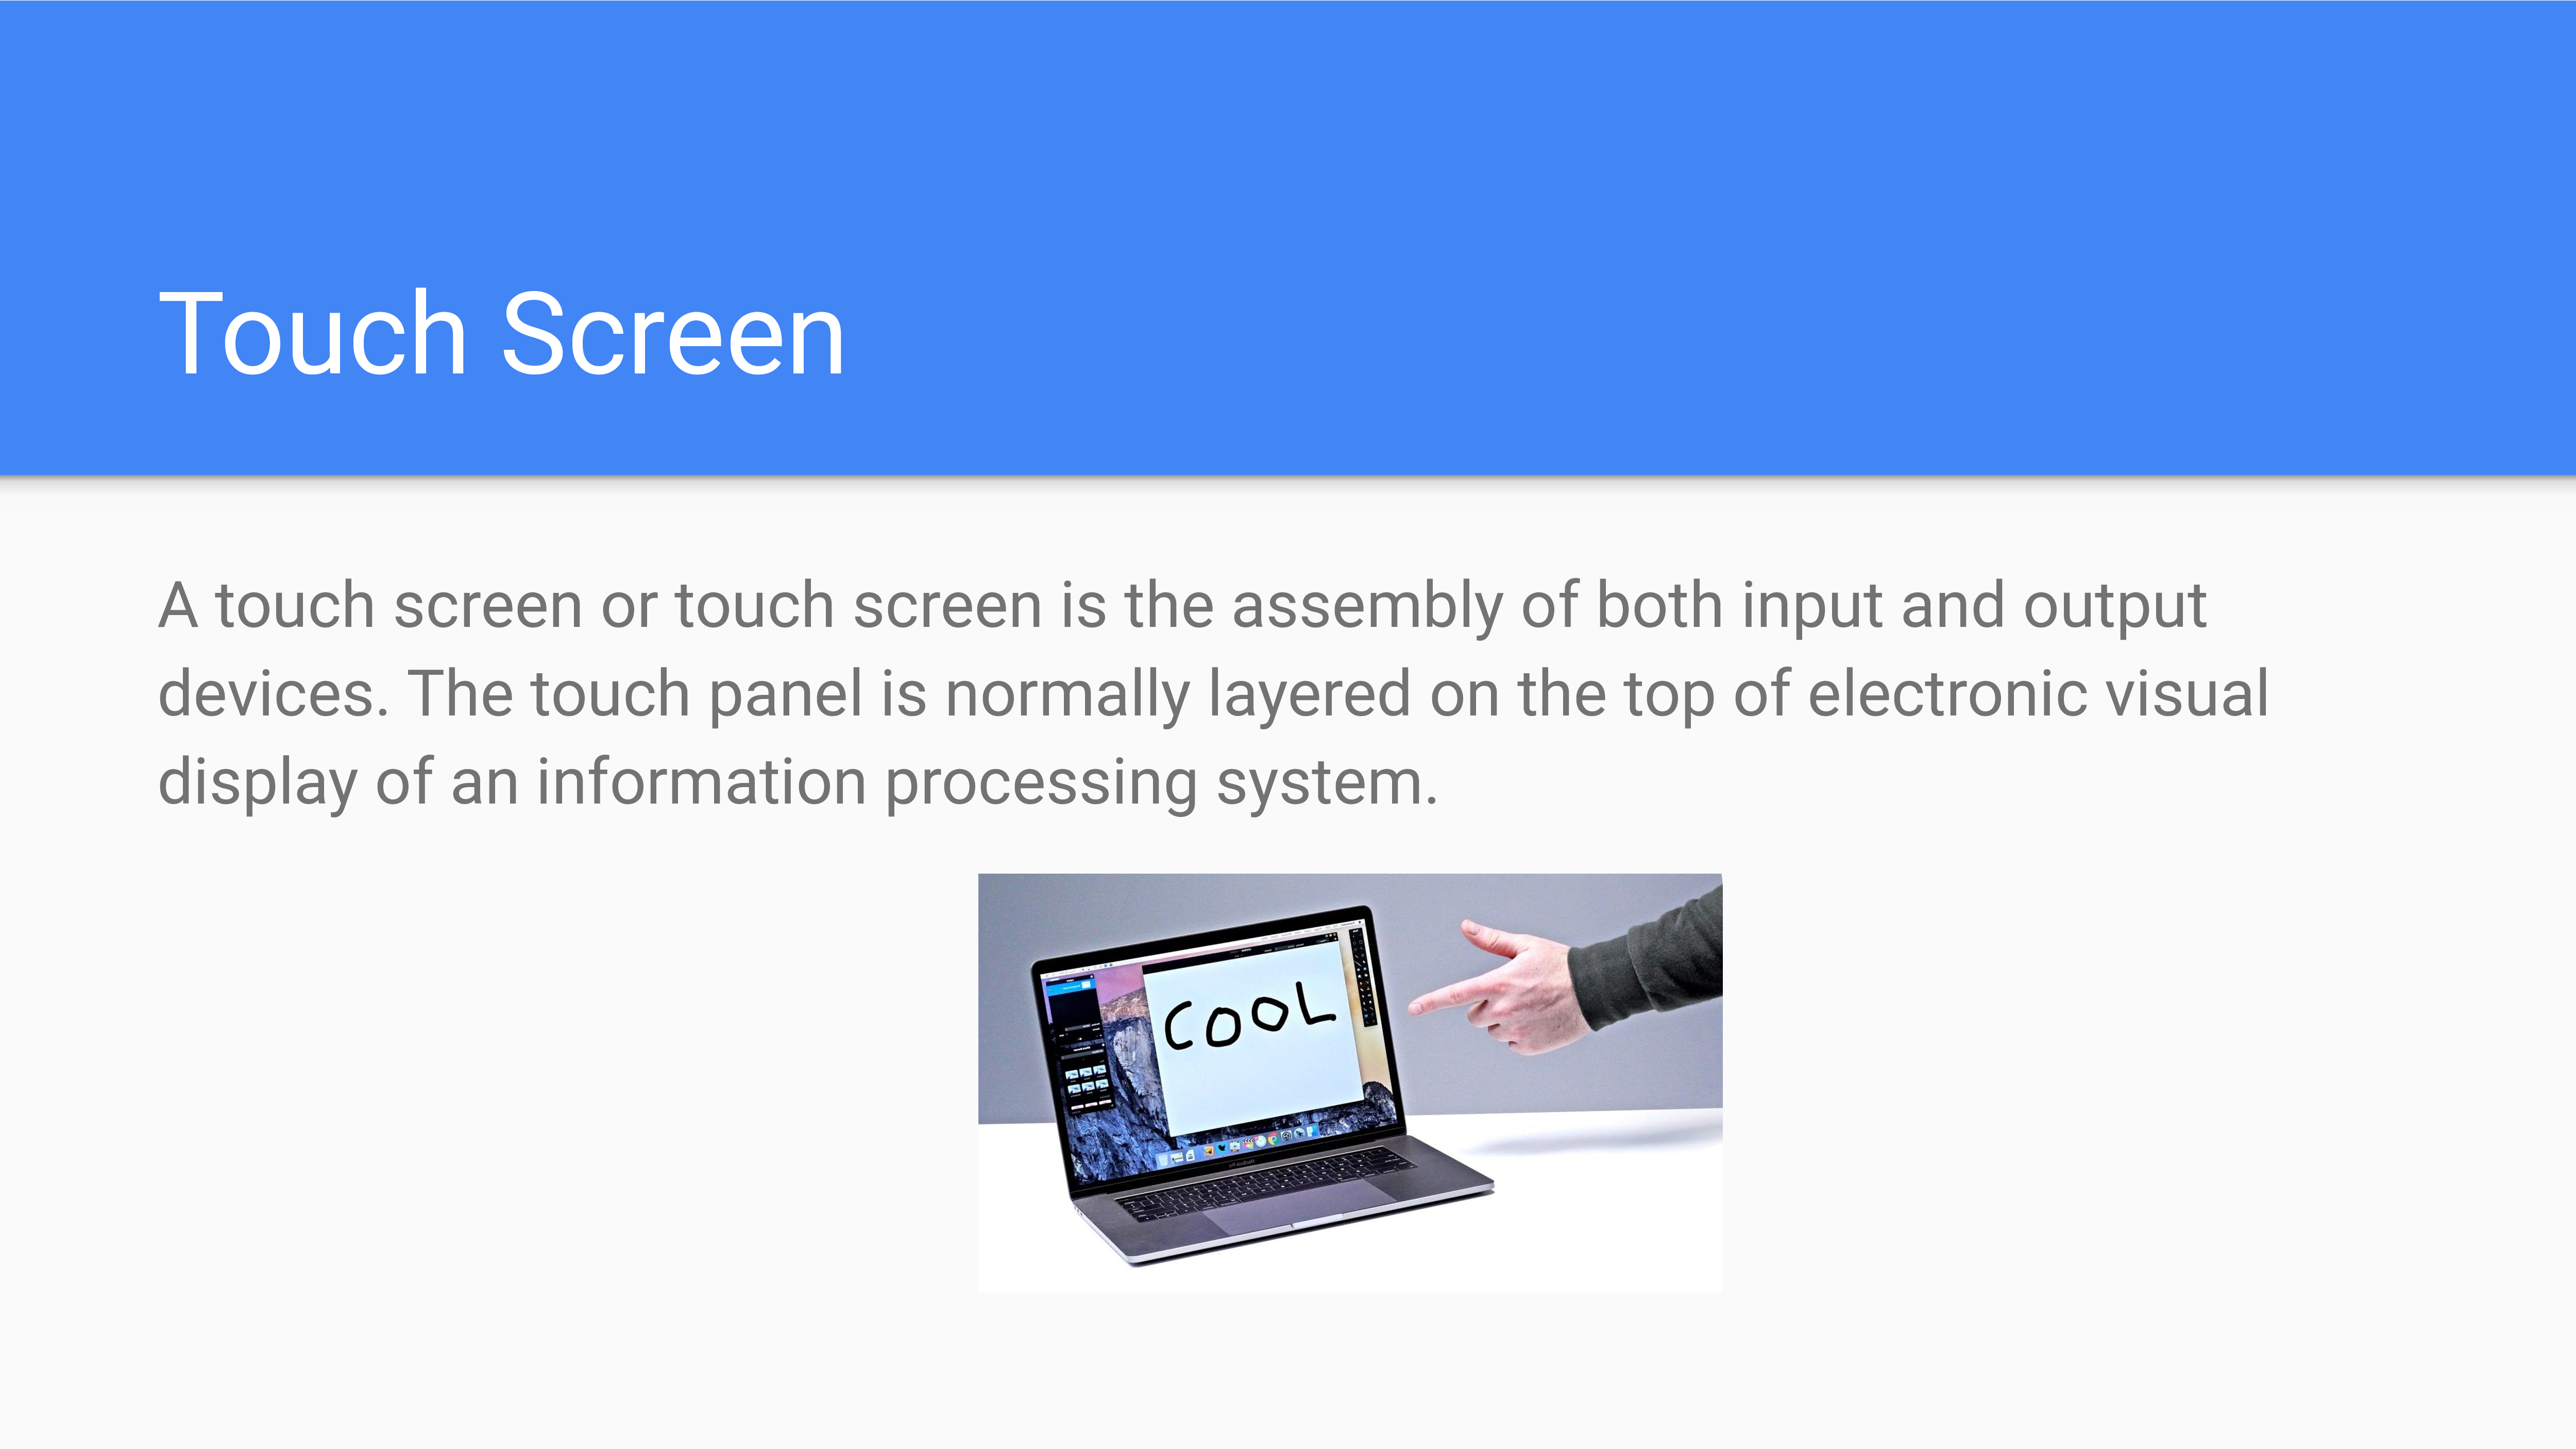
\includegraphics[width=0.7\linewidth]{./scrot/input-5.png}
	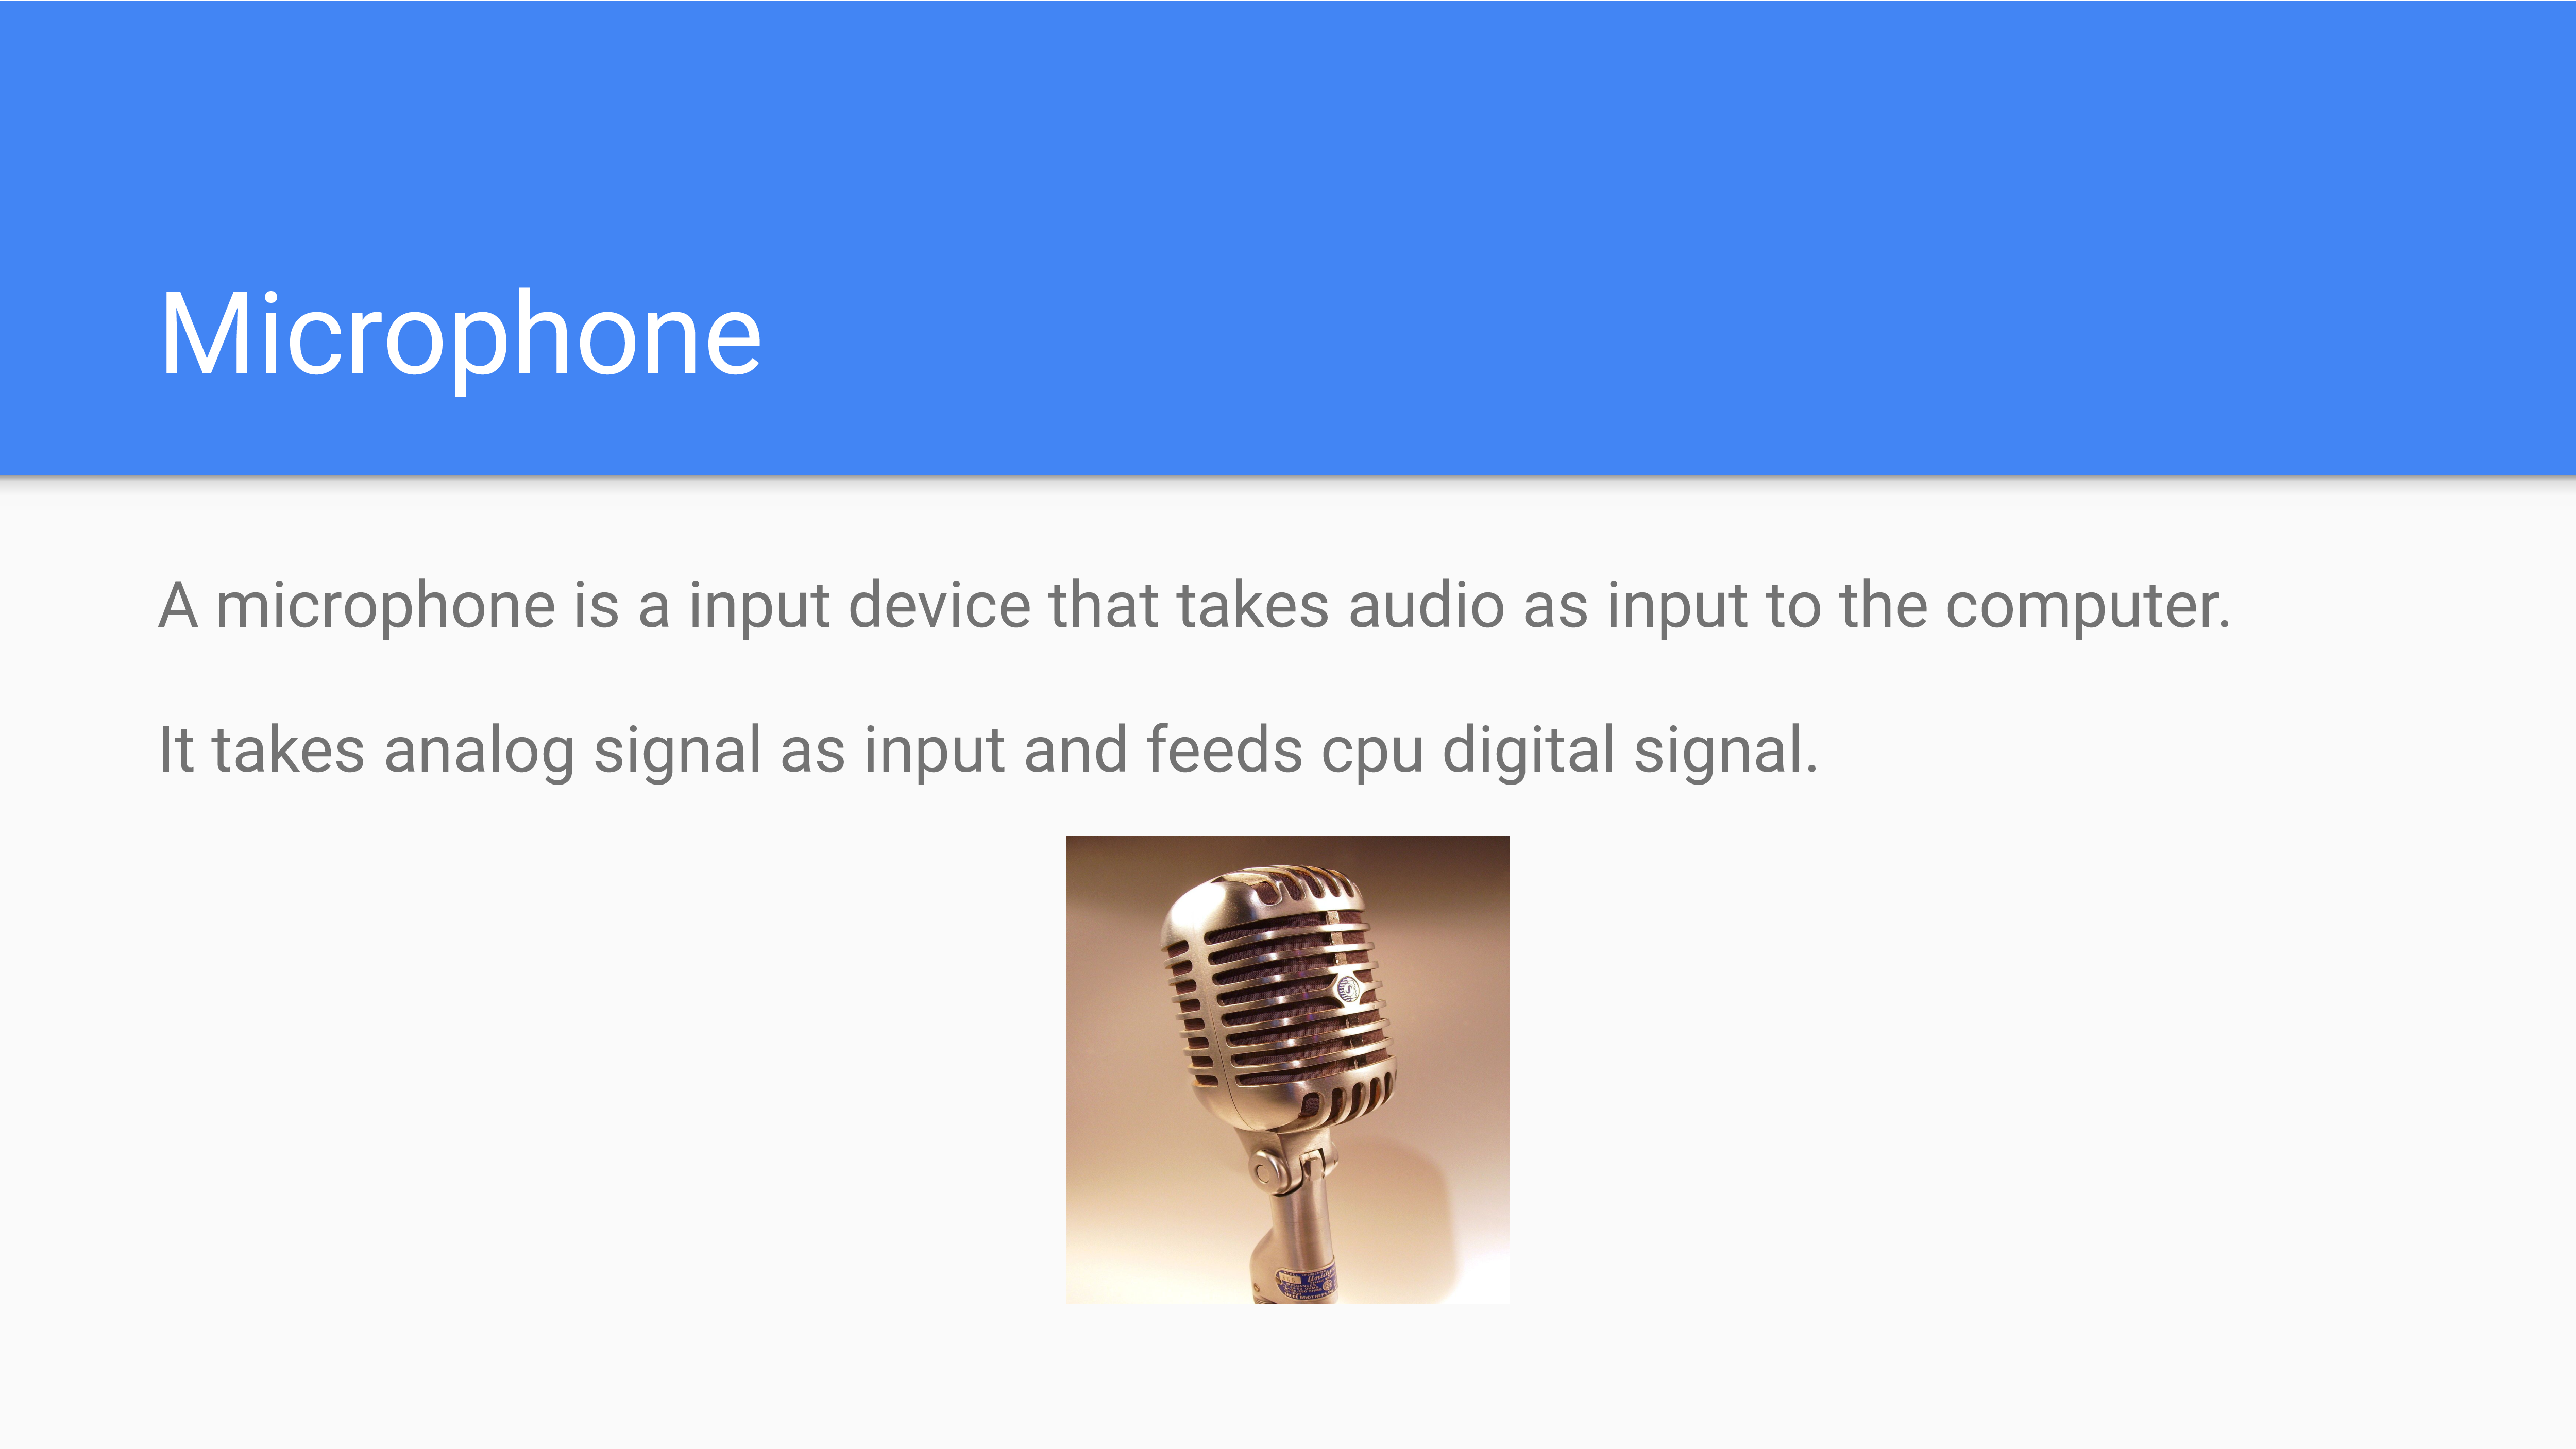
\includegraphics[width=0.7\linewidth]{./scrot/input-6.png}
	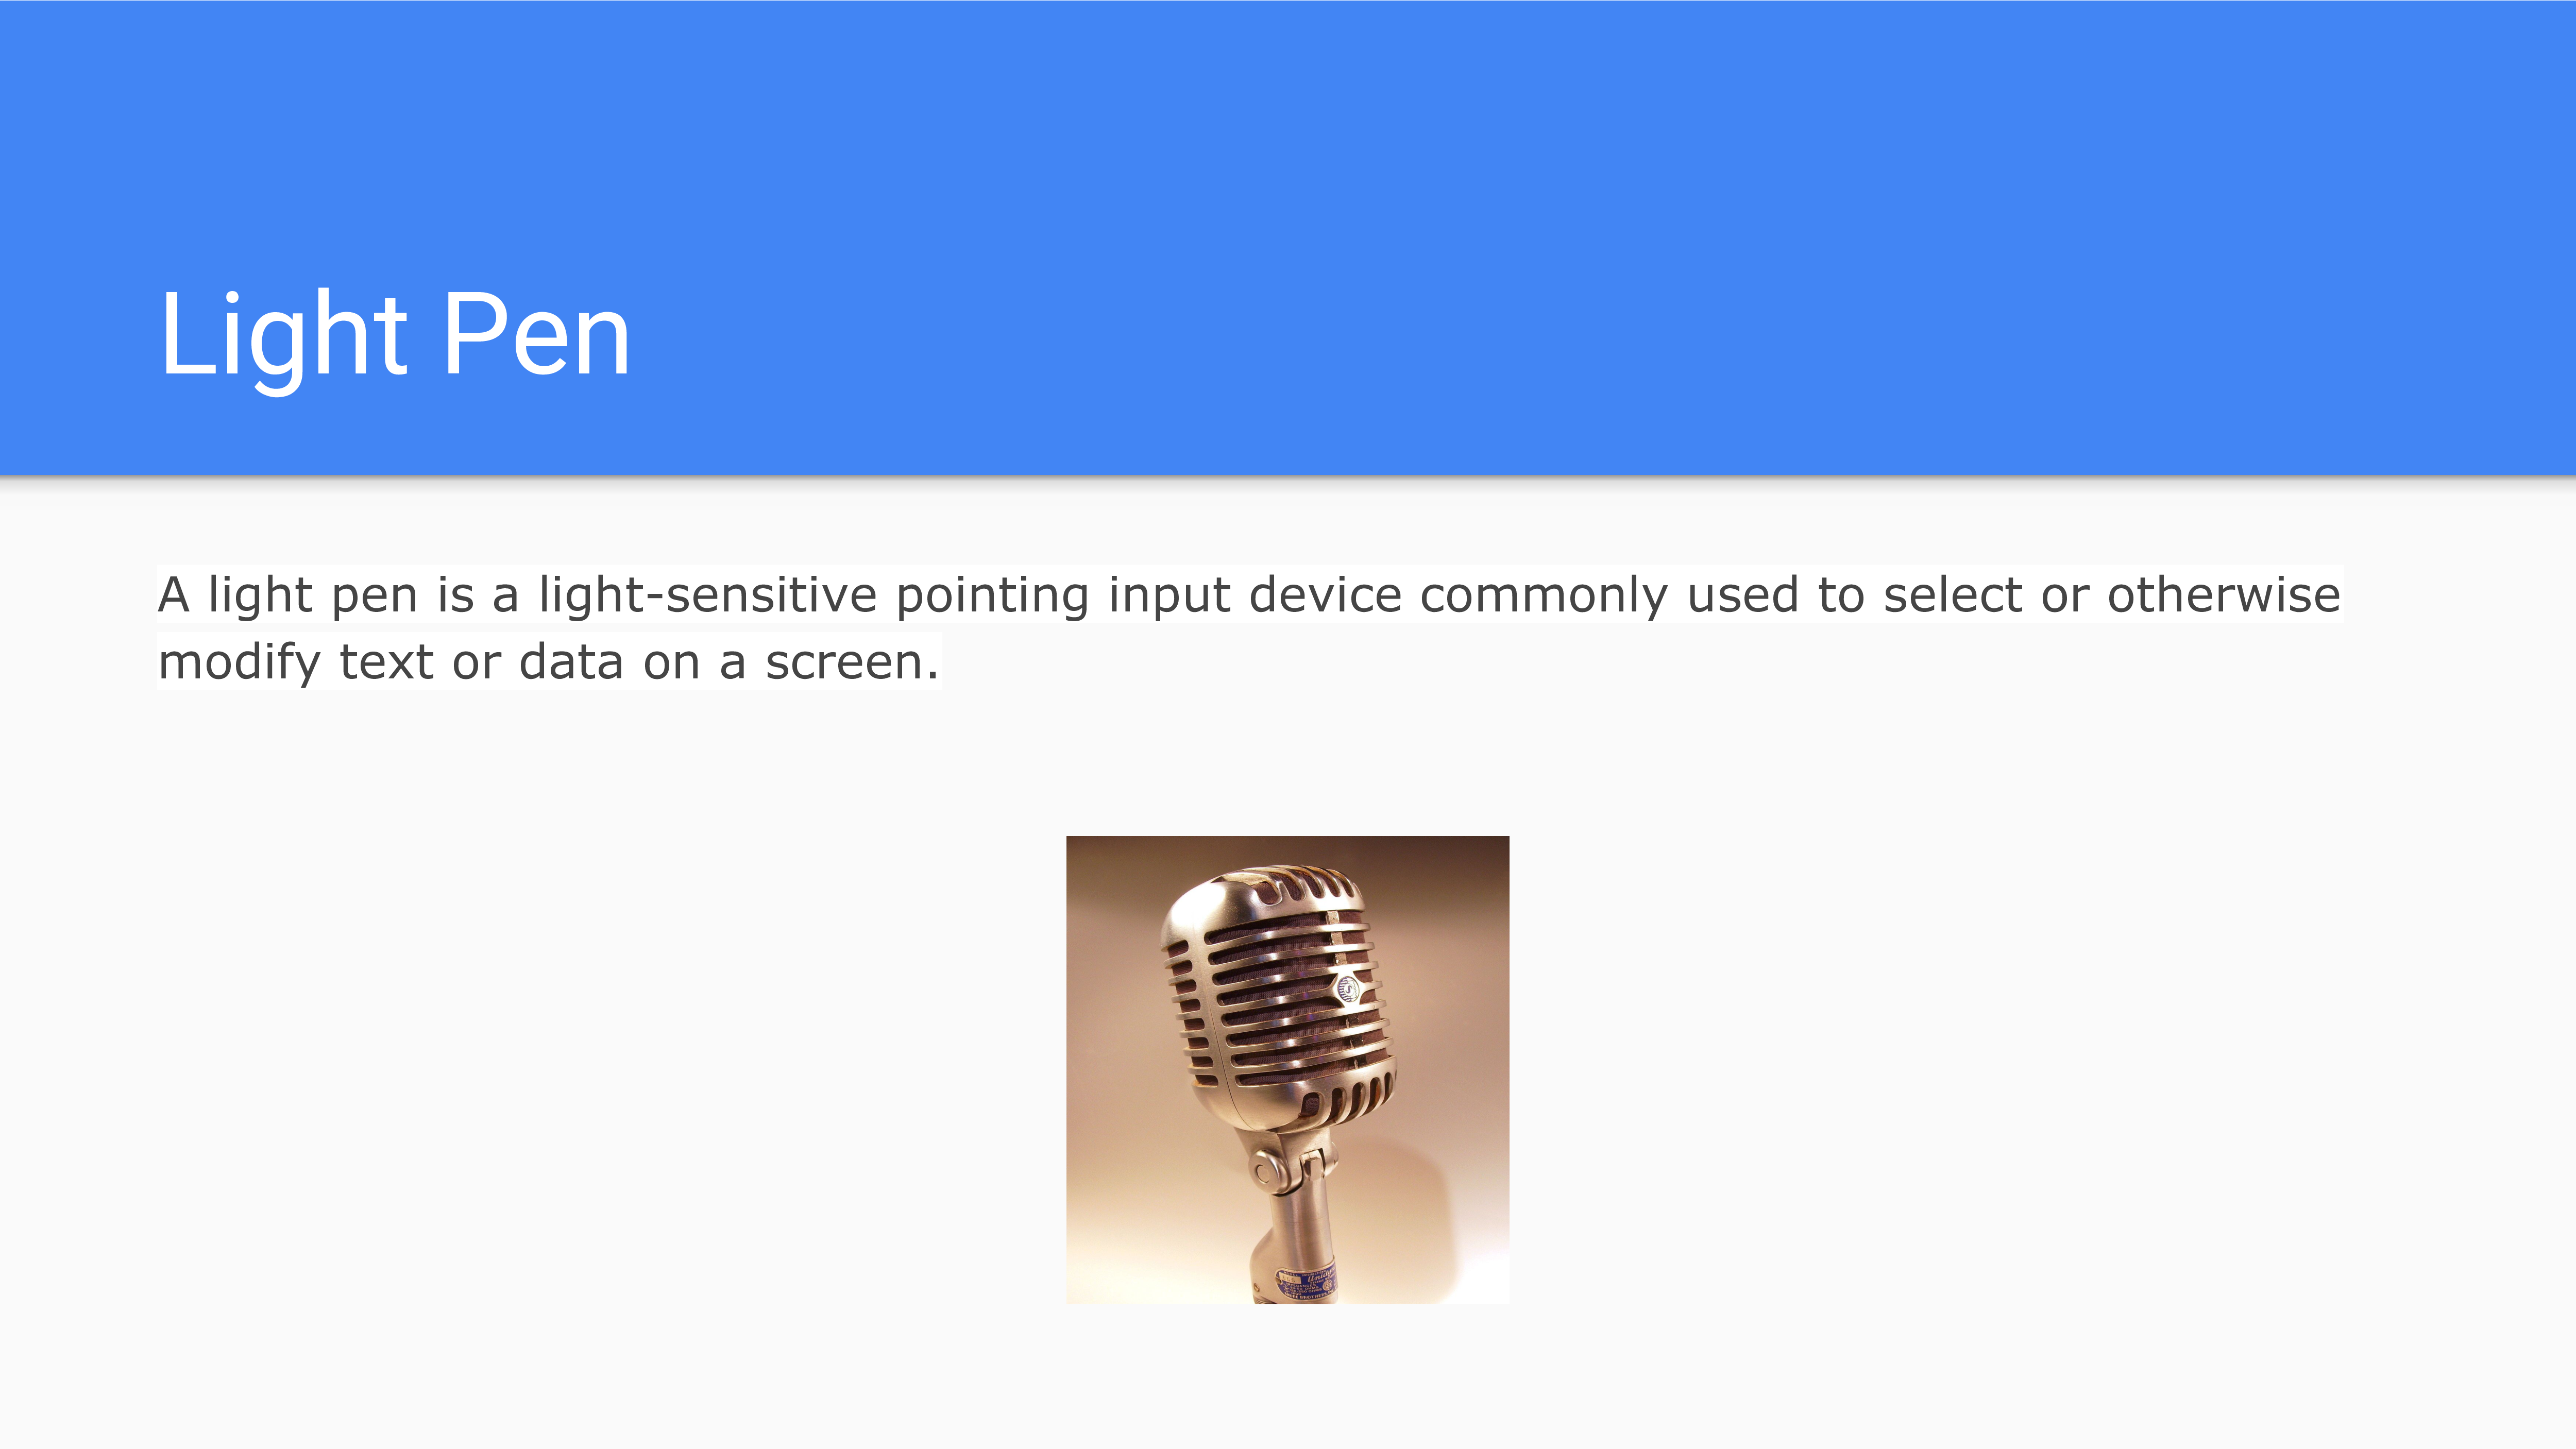
\includegraphics[width=0.7\linewidth]{./scrot/input-7.png}
\end{center}

\subsection{Multimedia}
\begin{center}
	
\includegraphics[width=0.7\linewidth]{./scrot/multimedia-0.png}
	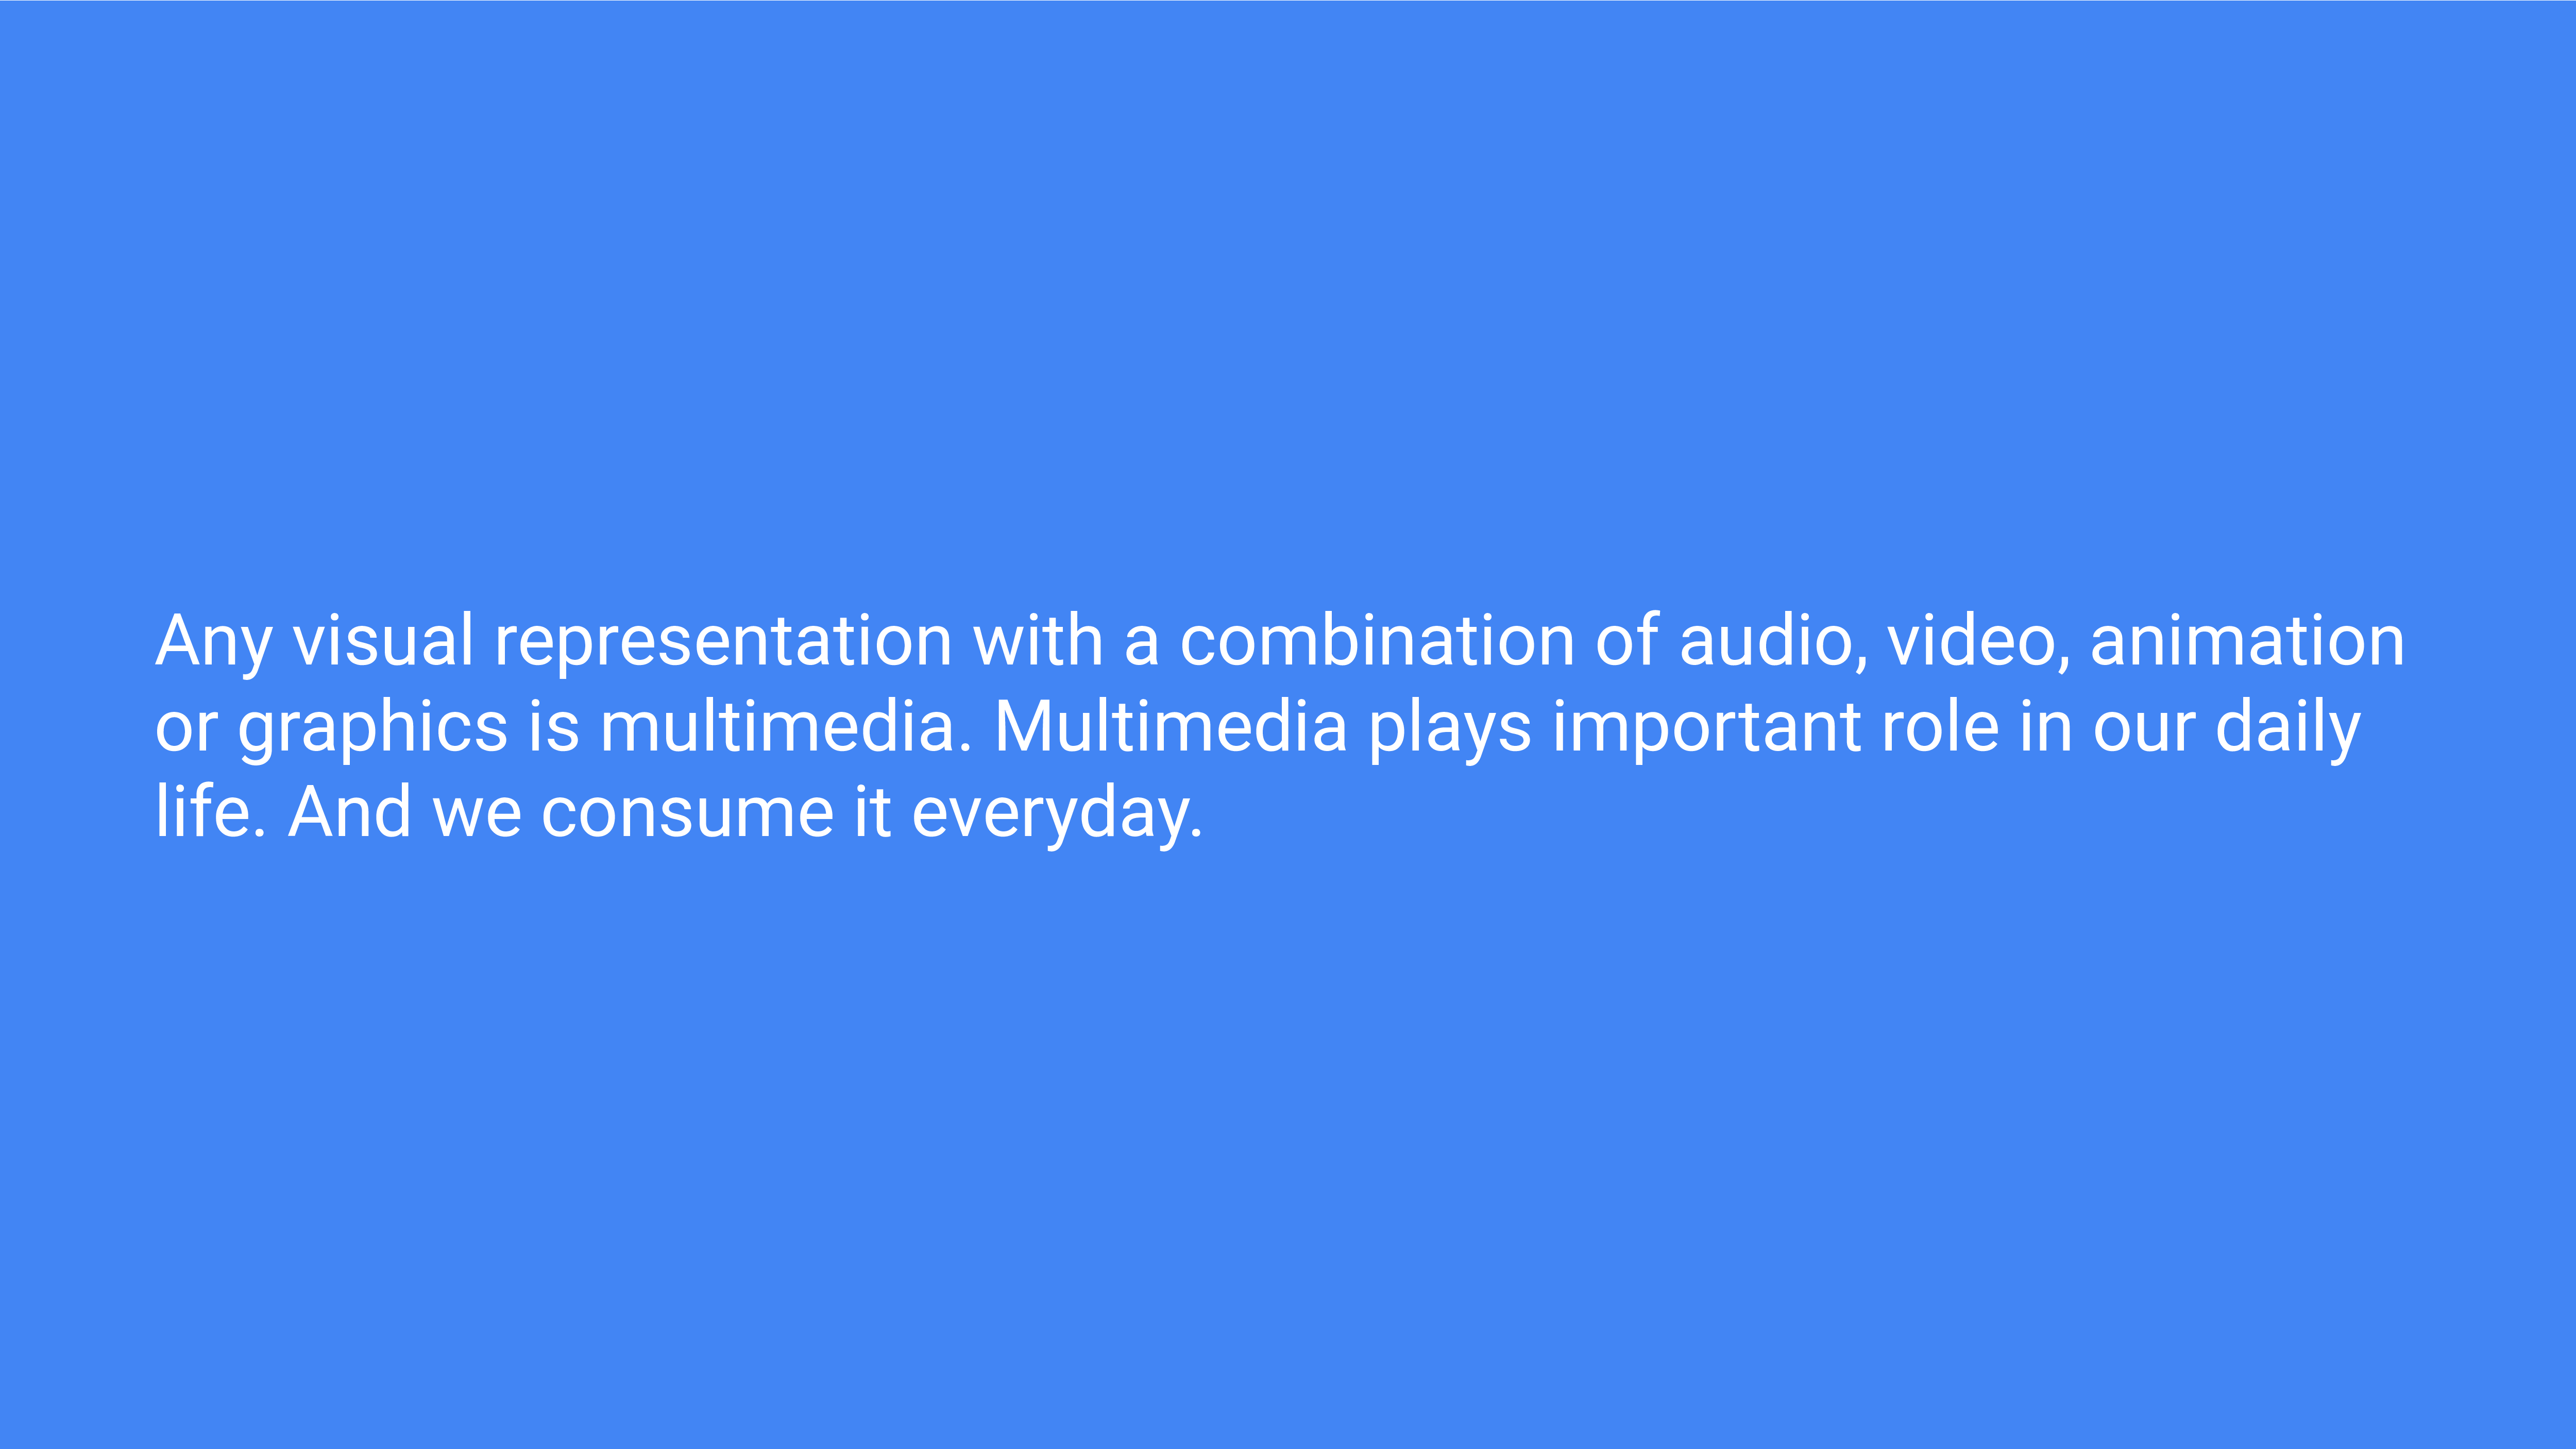
\includegraphics[width=0.7\linewidth]{./scrot/multimedia-1.png}
	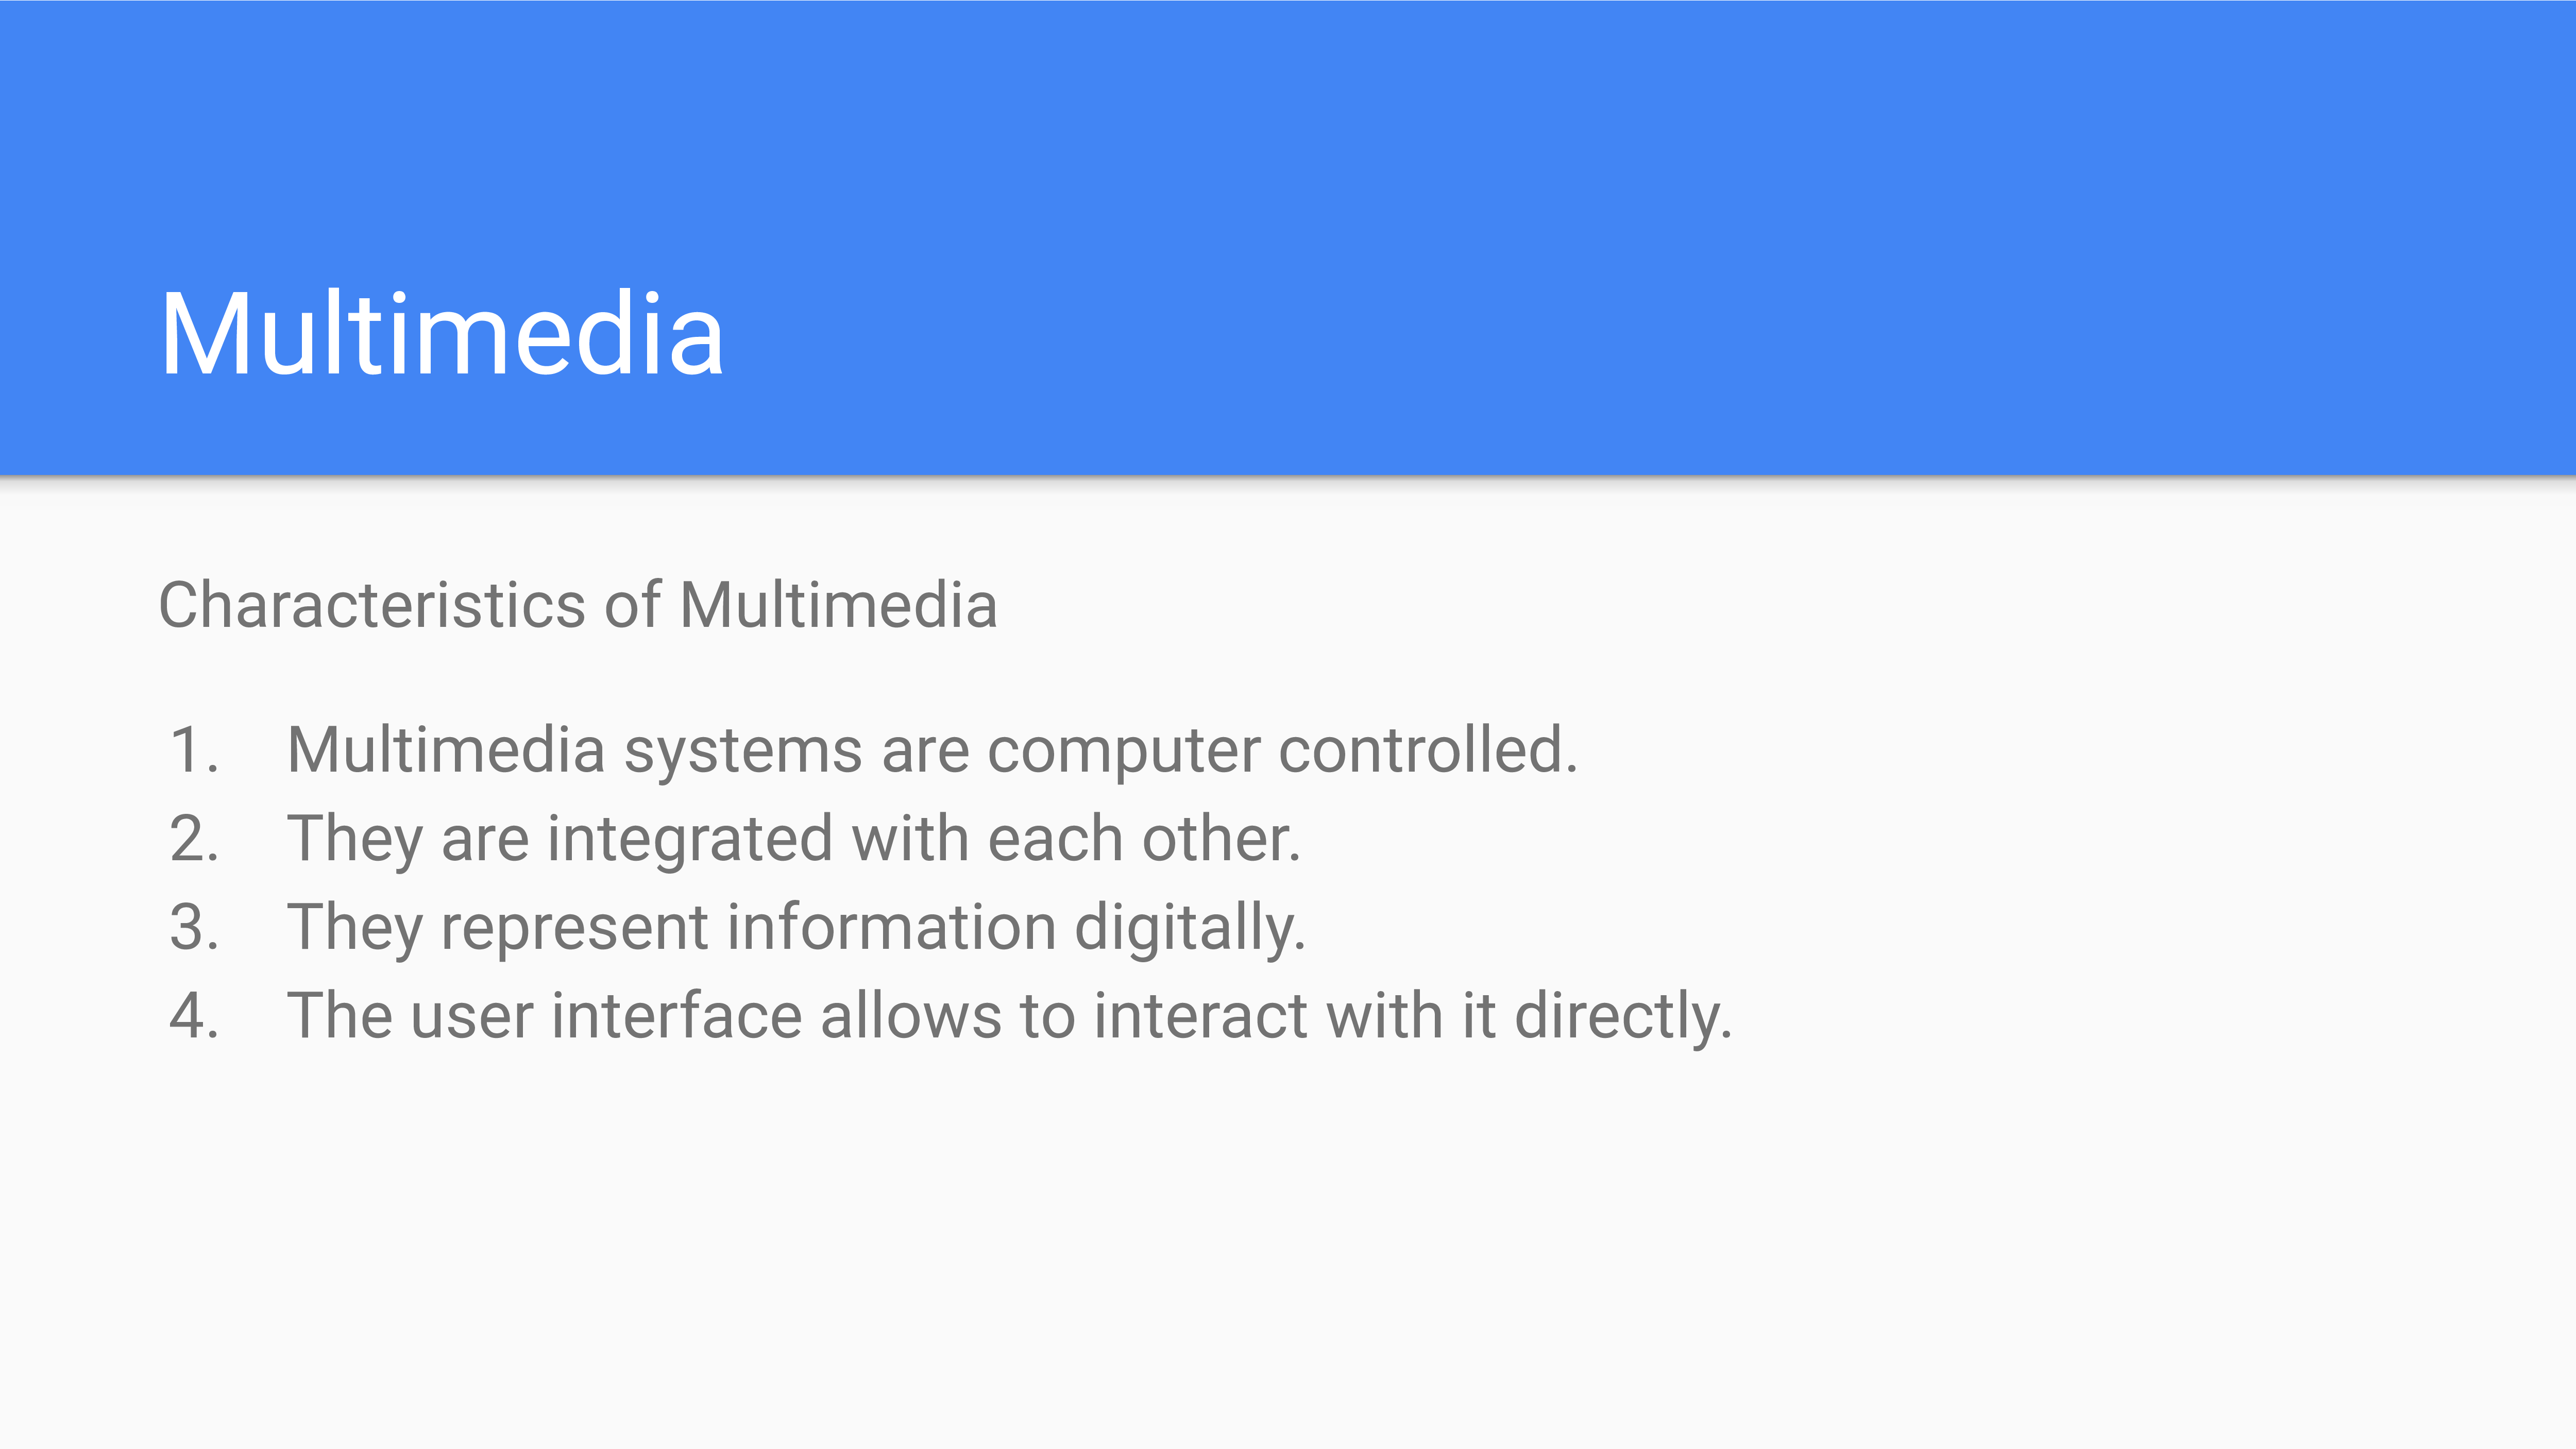
\includegraphics[width=0.7\linewidth]{./scrot/multimedia-2.png}
	
\includegraphics[width=0.7\linewidth]{./scrot/multimedia-3.png}
\end{center}
\begin{center}
	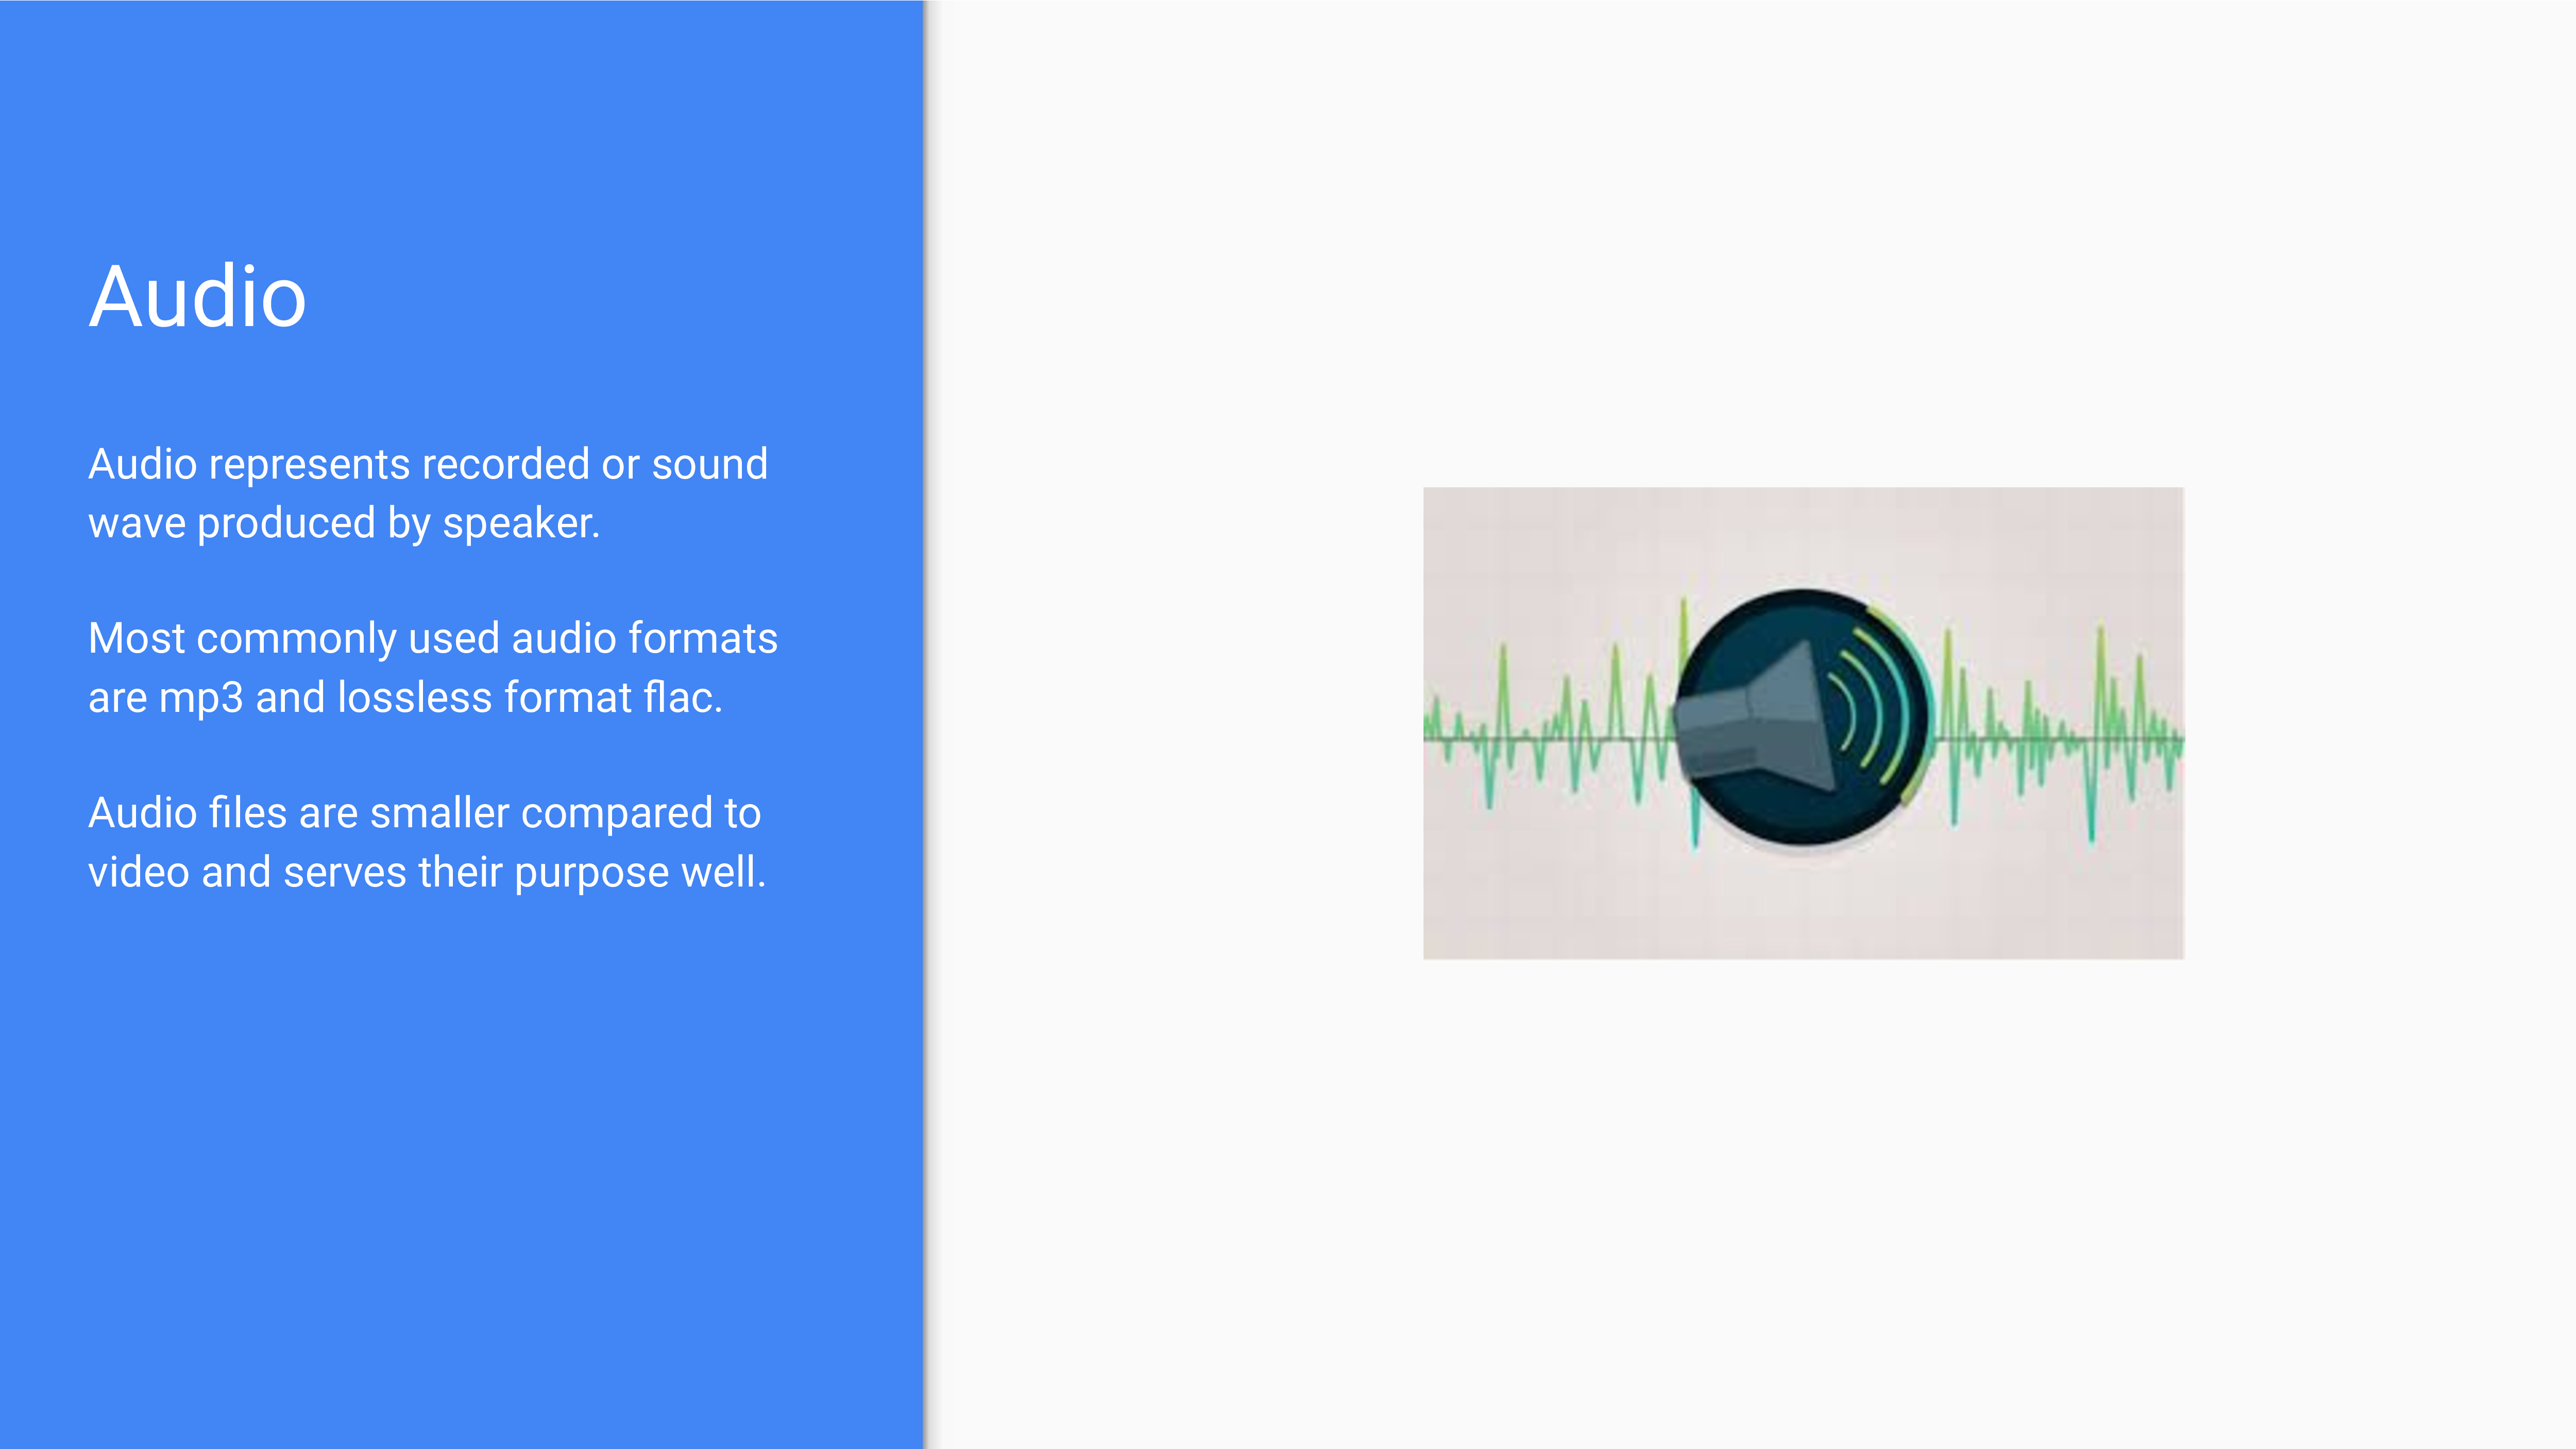
\includegraphics[width=0.7\linewidth]{./scrot/multimedia-4.png}
	
\includegraphics[width=0.7\linewidth]{./scrot/multimedia-5.png}
	
\includegraphics[width=0.7\linewidth]{./scrot/multimedia-6.png}
	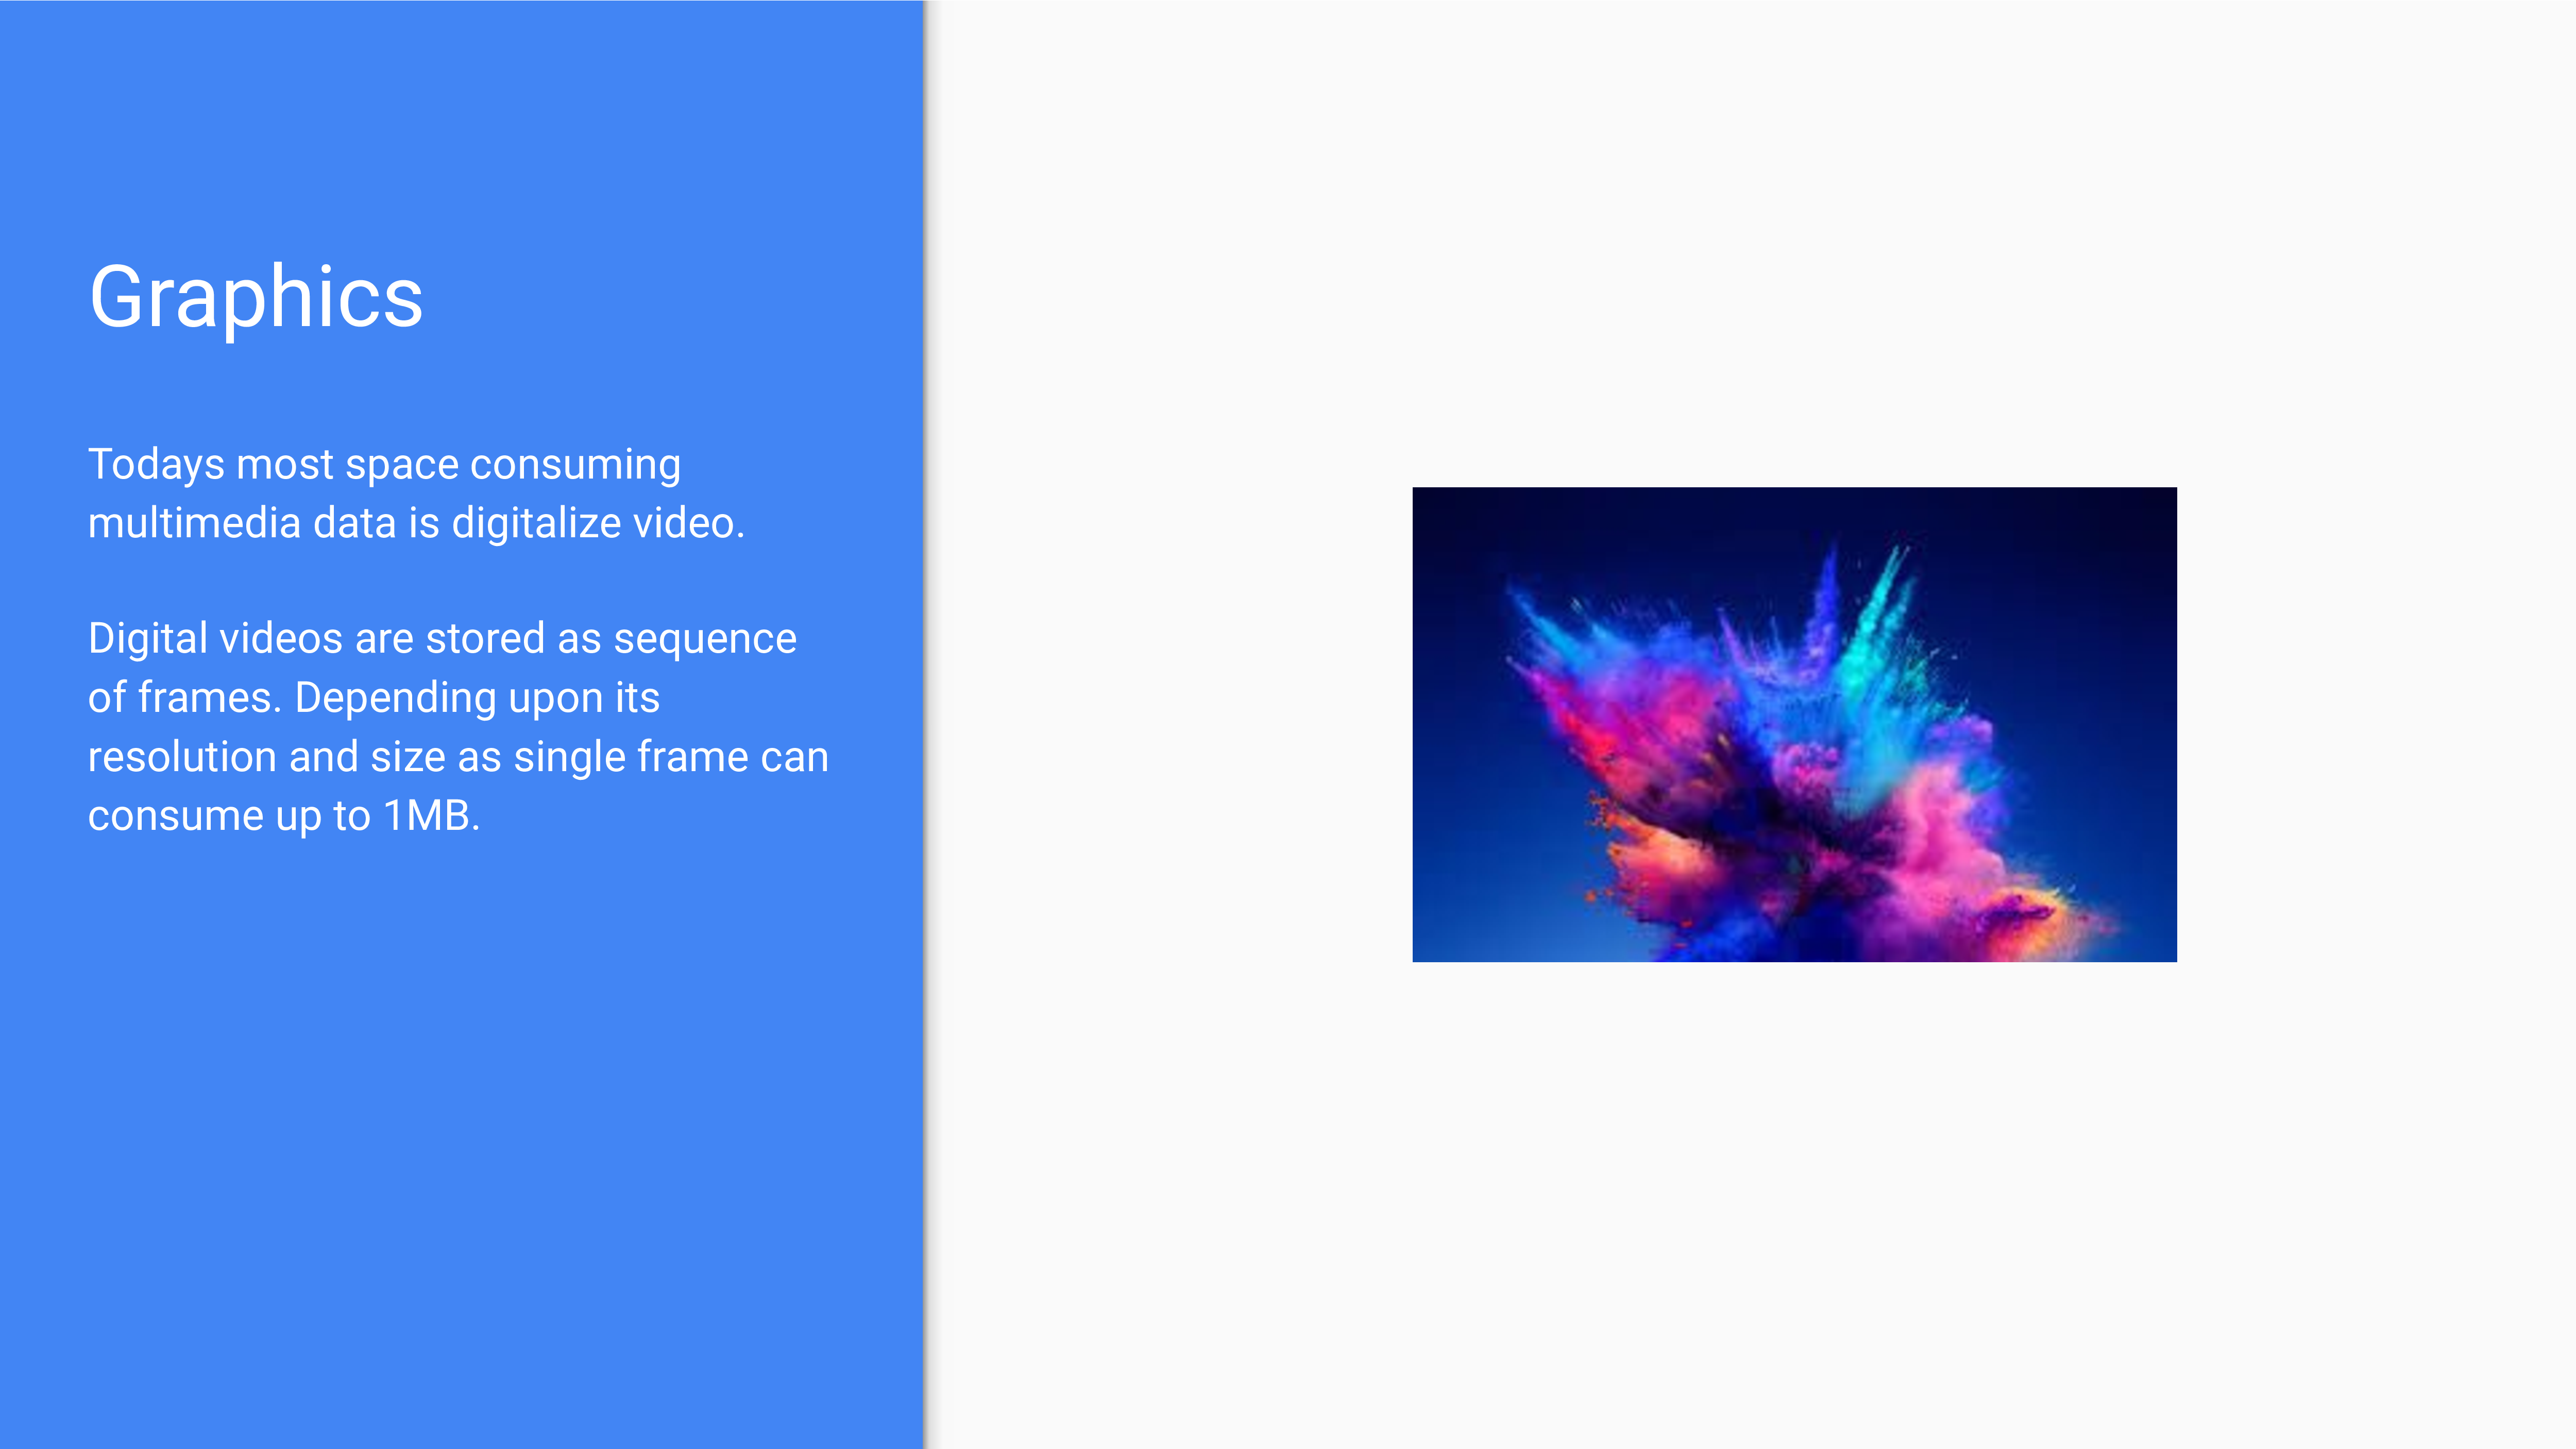
\includegraphics[width=0.7\linewidth]{./scrot/multimedia-7.png}
\end{center}

\subsection{Cloud Computing}
\begin{center}
	
\includegraphics[width=0.7\linewidth]{./scrot/cloud.png}
	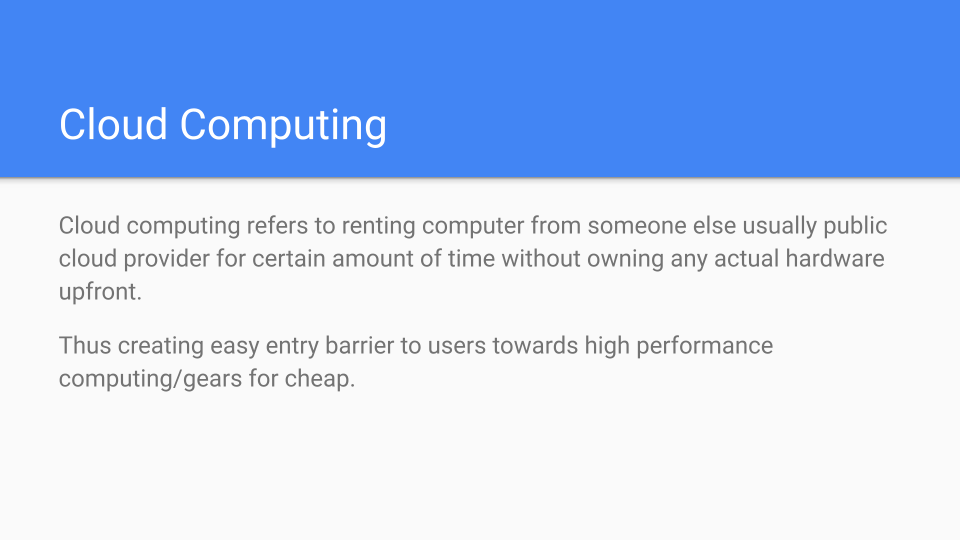
\includegraphics[width=0.7\linewidth]{./scrot/cloud1.png}
	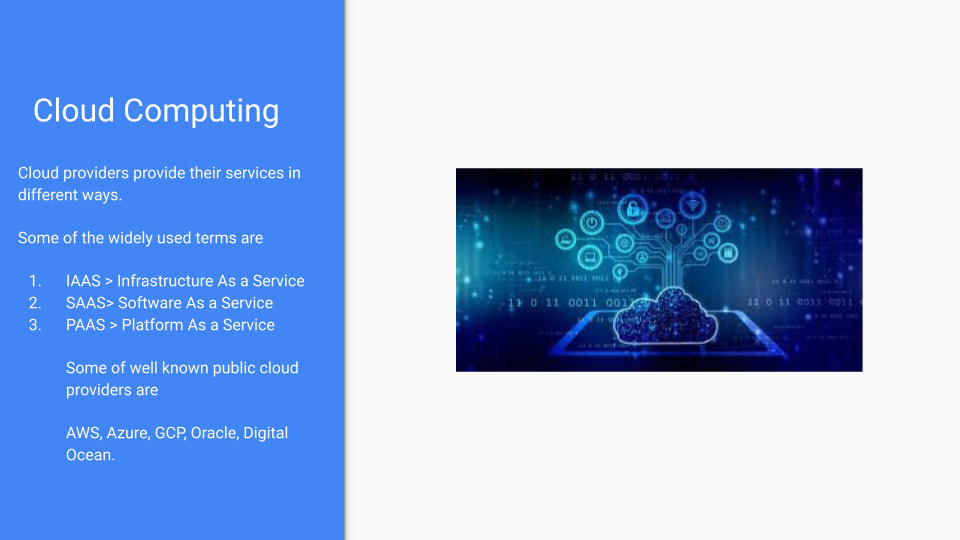
\includegraphics[width=0.7\linewidth]{./scrot/cloud2.png}
	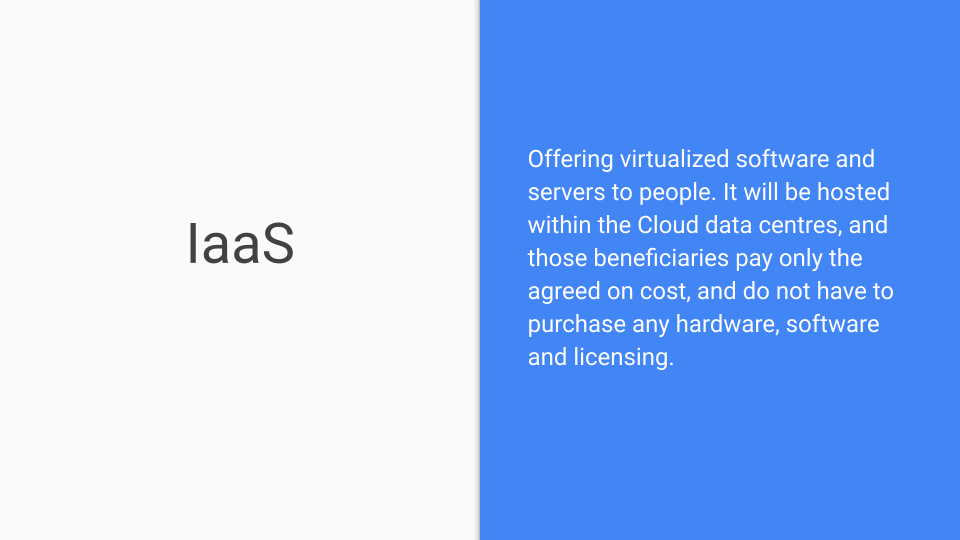
\includegraphics[width=0.7\linewidth]{./scrot/cloud3.png}
\end{center}
\begin{center}
	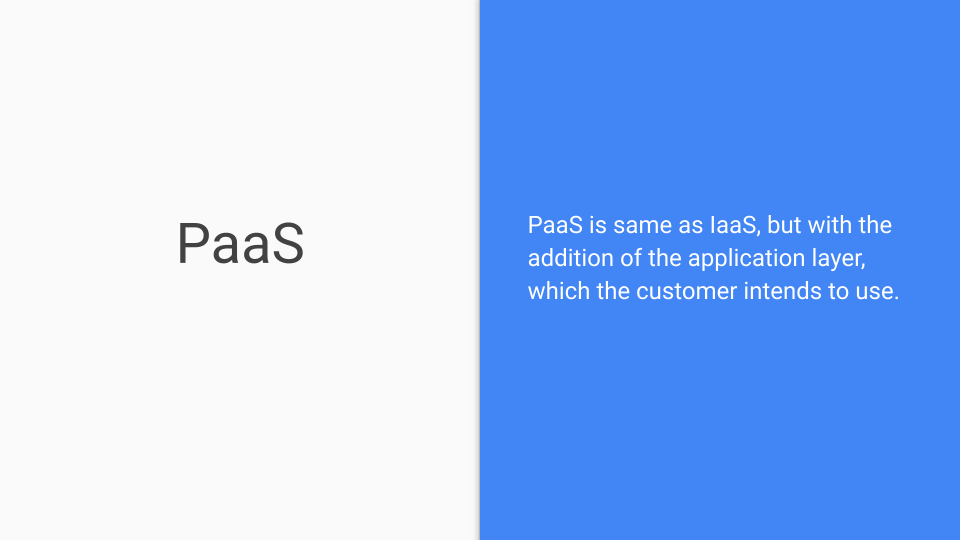
\includegraphics[width=0.7\linewidth]{./scrot/cloud4.png}
	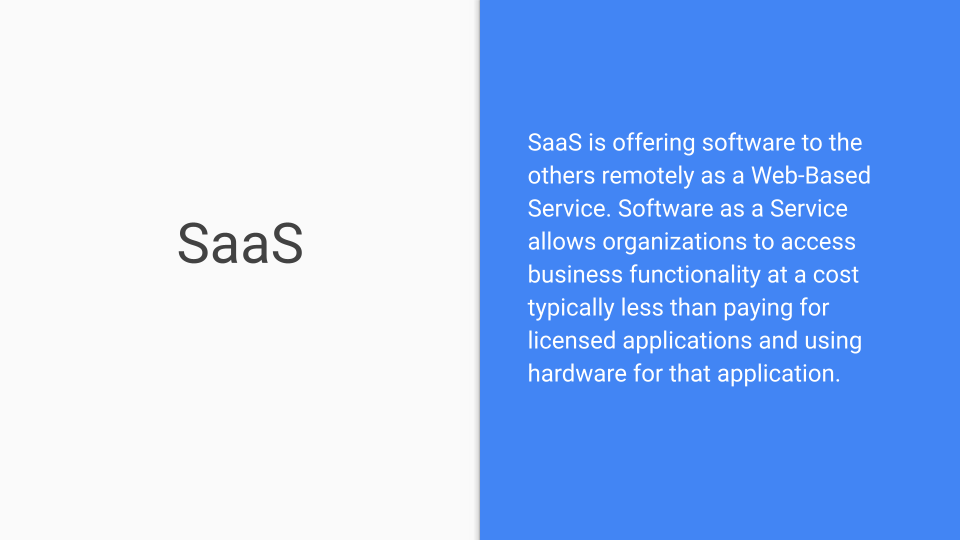
\includegraphics[width=0.7\linewidth]{./scrot/cloud5.png}
	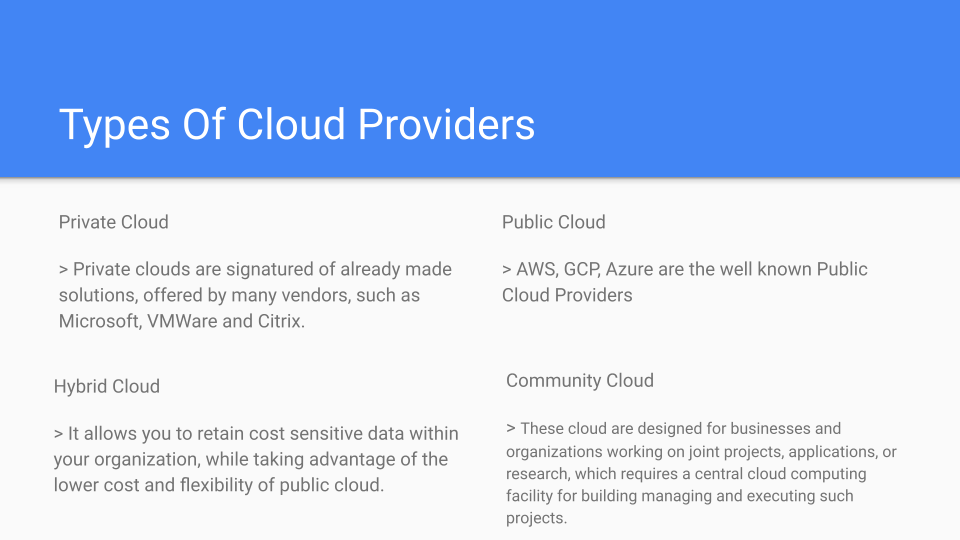
\includegraphics[width=0.7\linewidth]{./scrot/cloud6.png}
	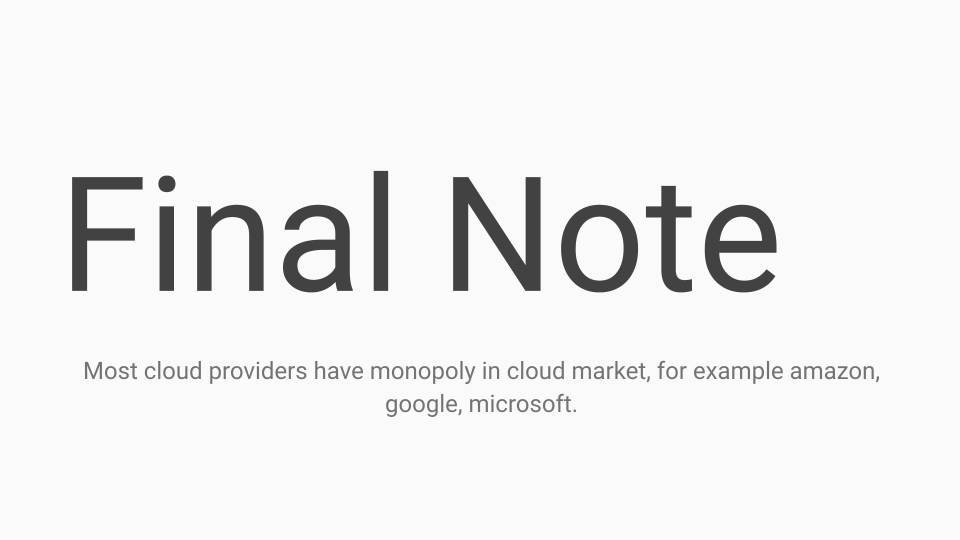
\includegraphics[width=0.7\linewidth]{./scrot/cloud7.png}
\end{center}

\subsection{Smart City}
\begin{center}
	
\includegraphics[width=0.7\linewidth]{./scrot/smart-city-0.png}
	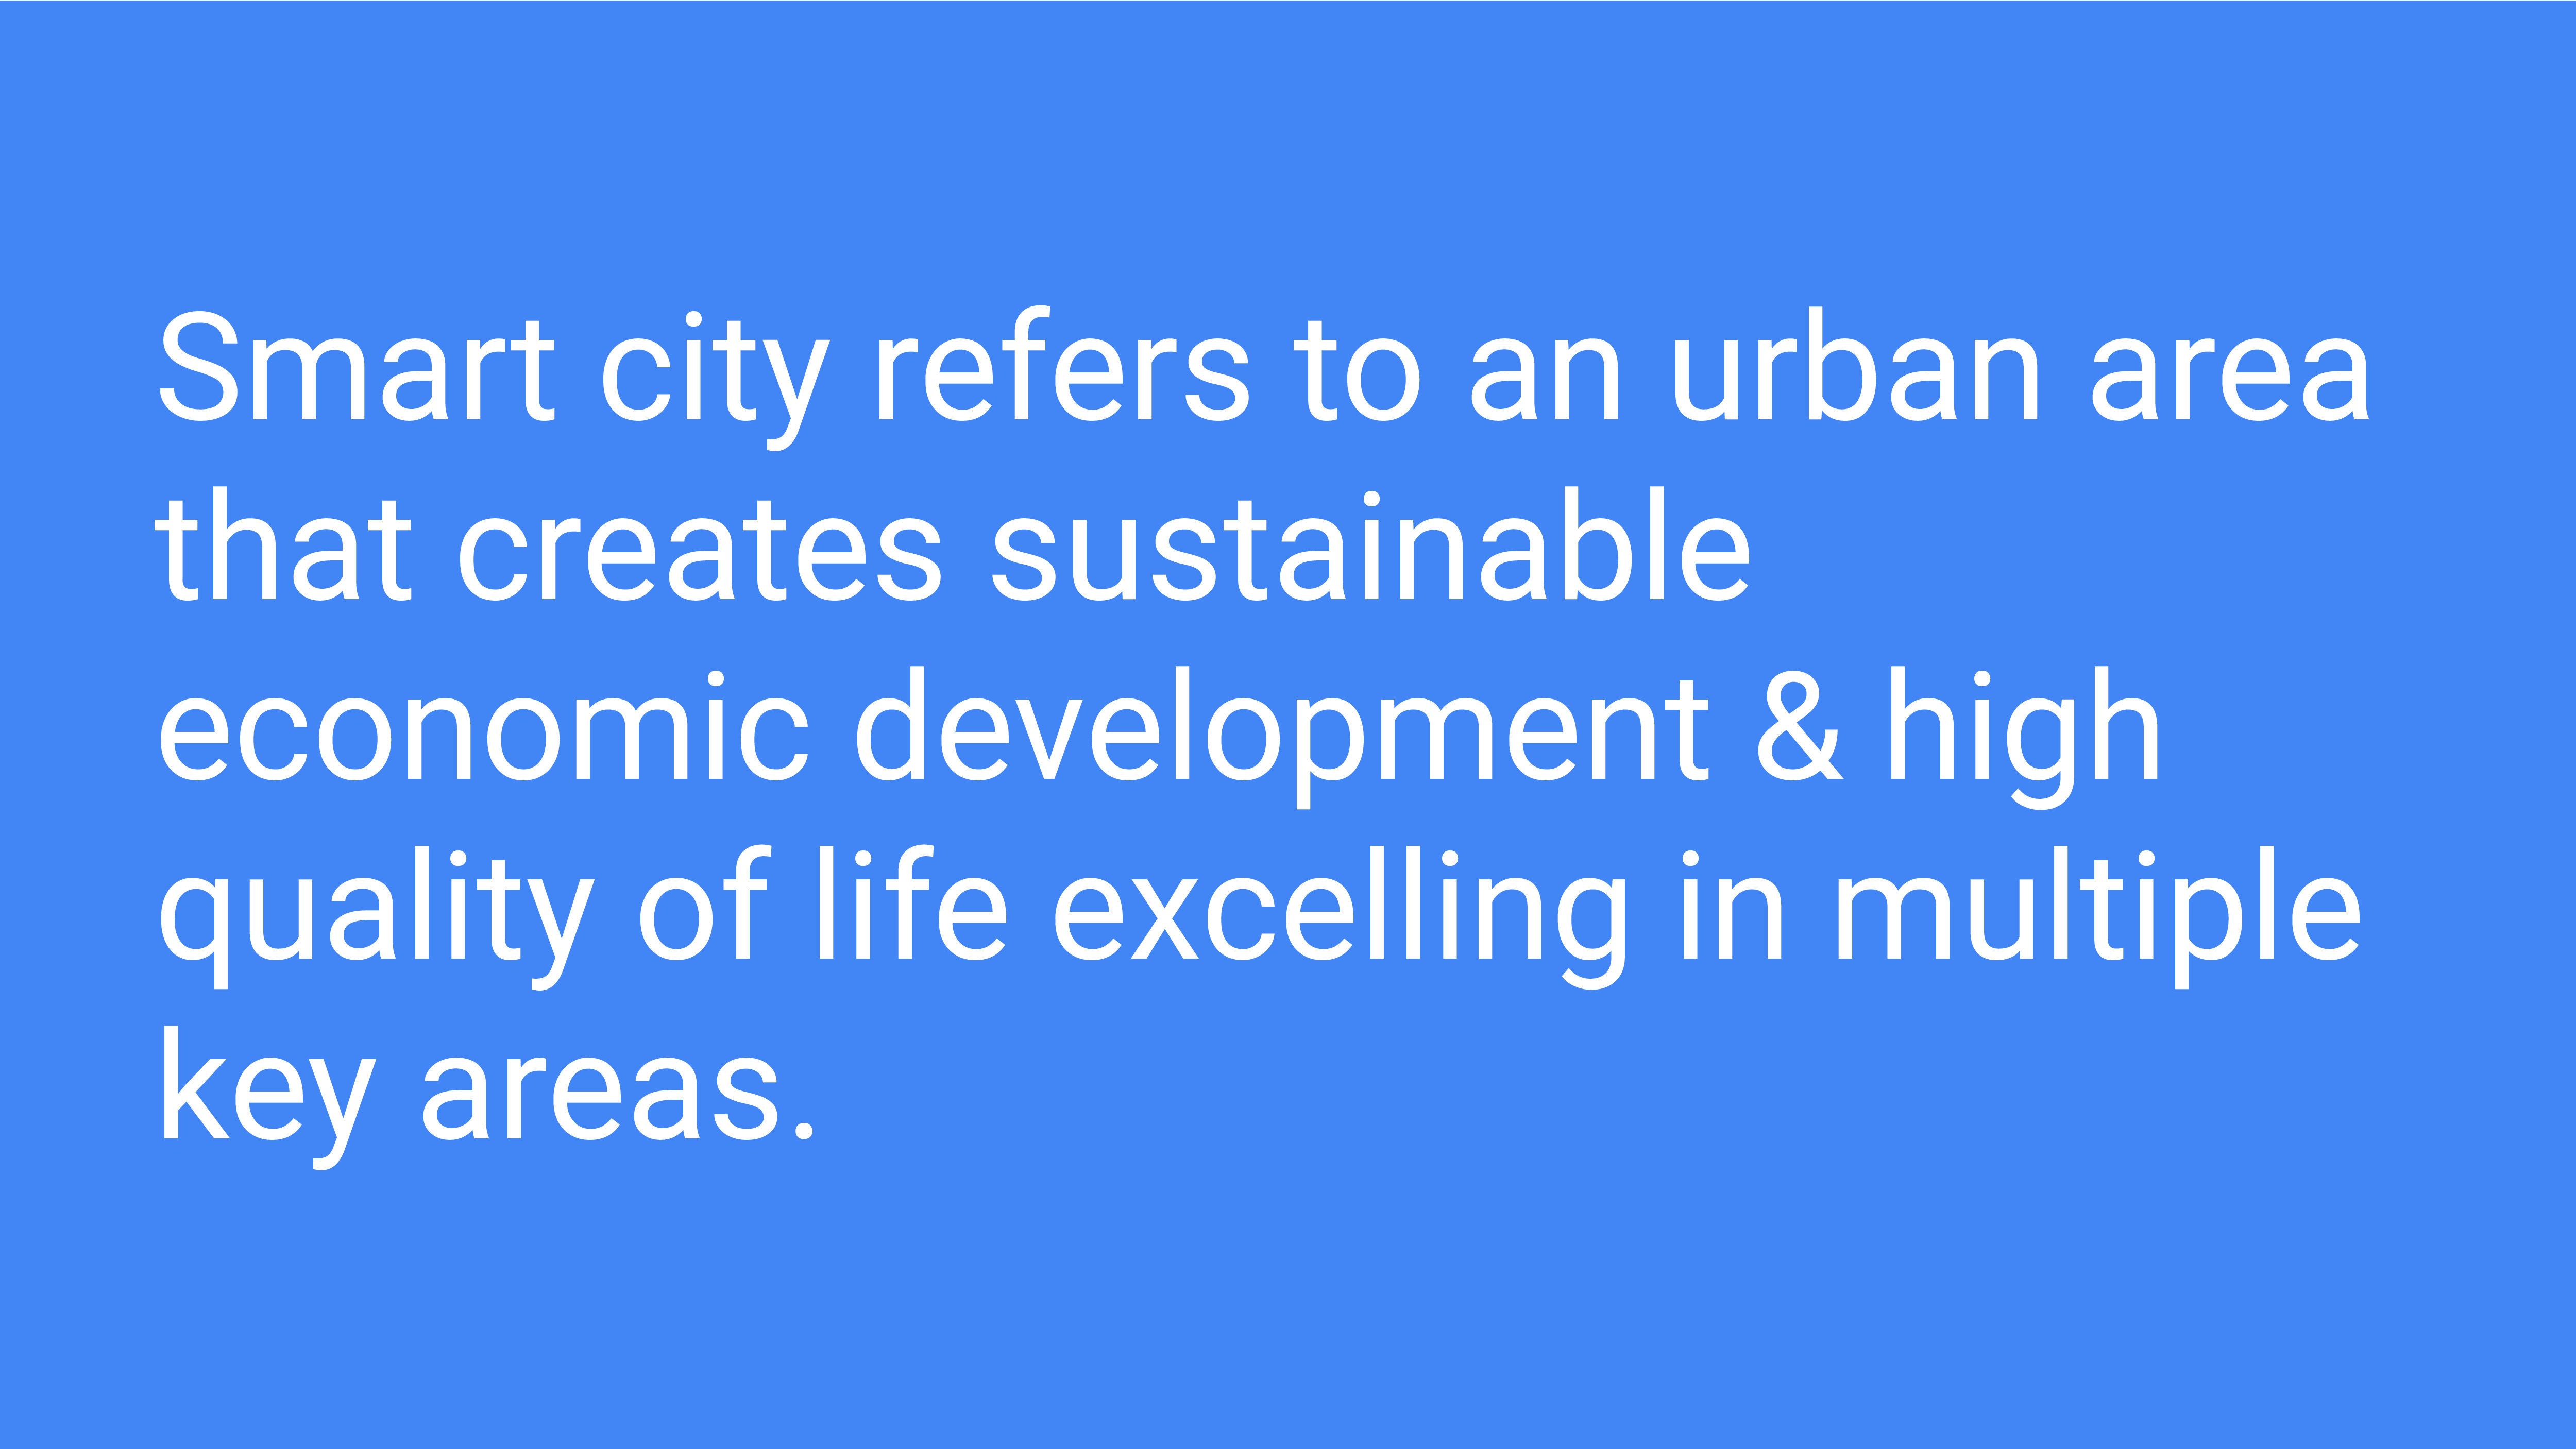
\includegraphics[width=0.7\linewidth]{./scrot/smart-city-1.png}
	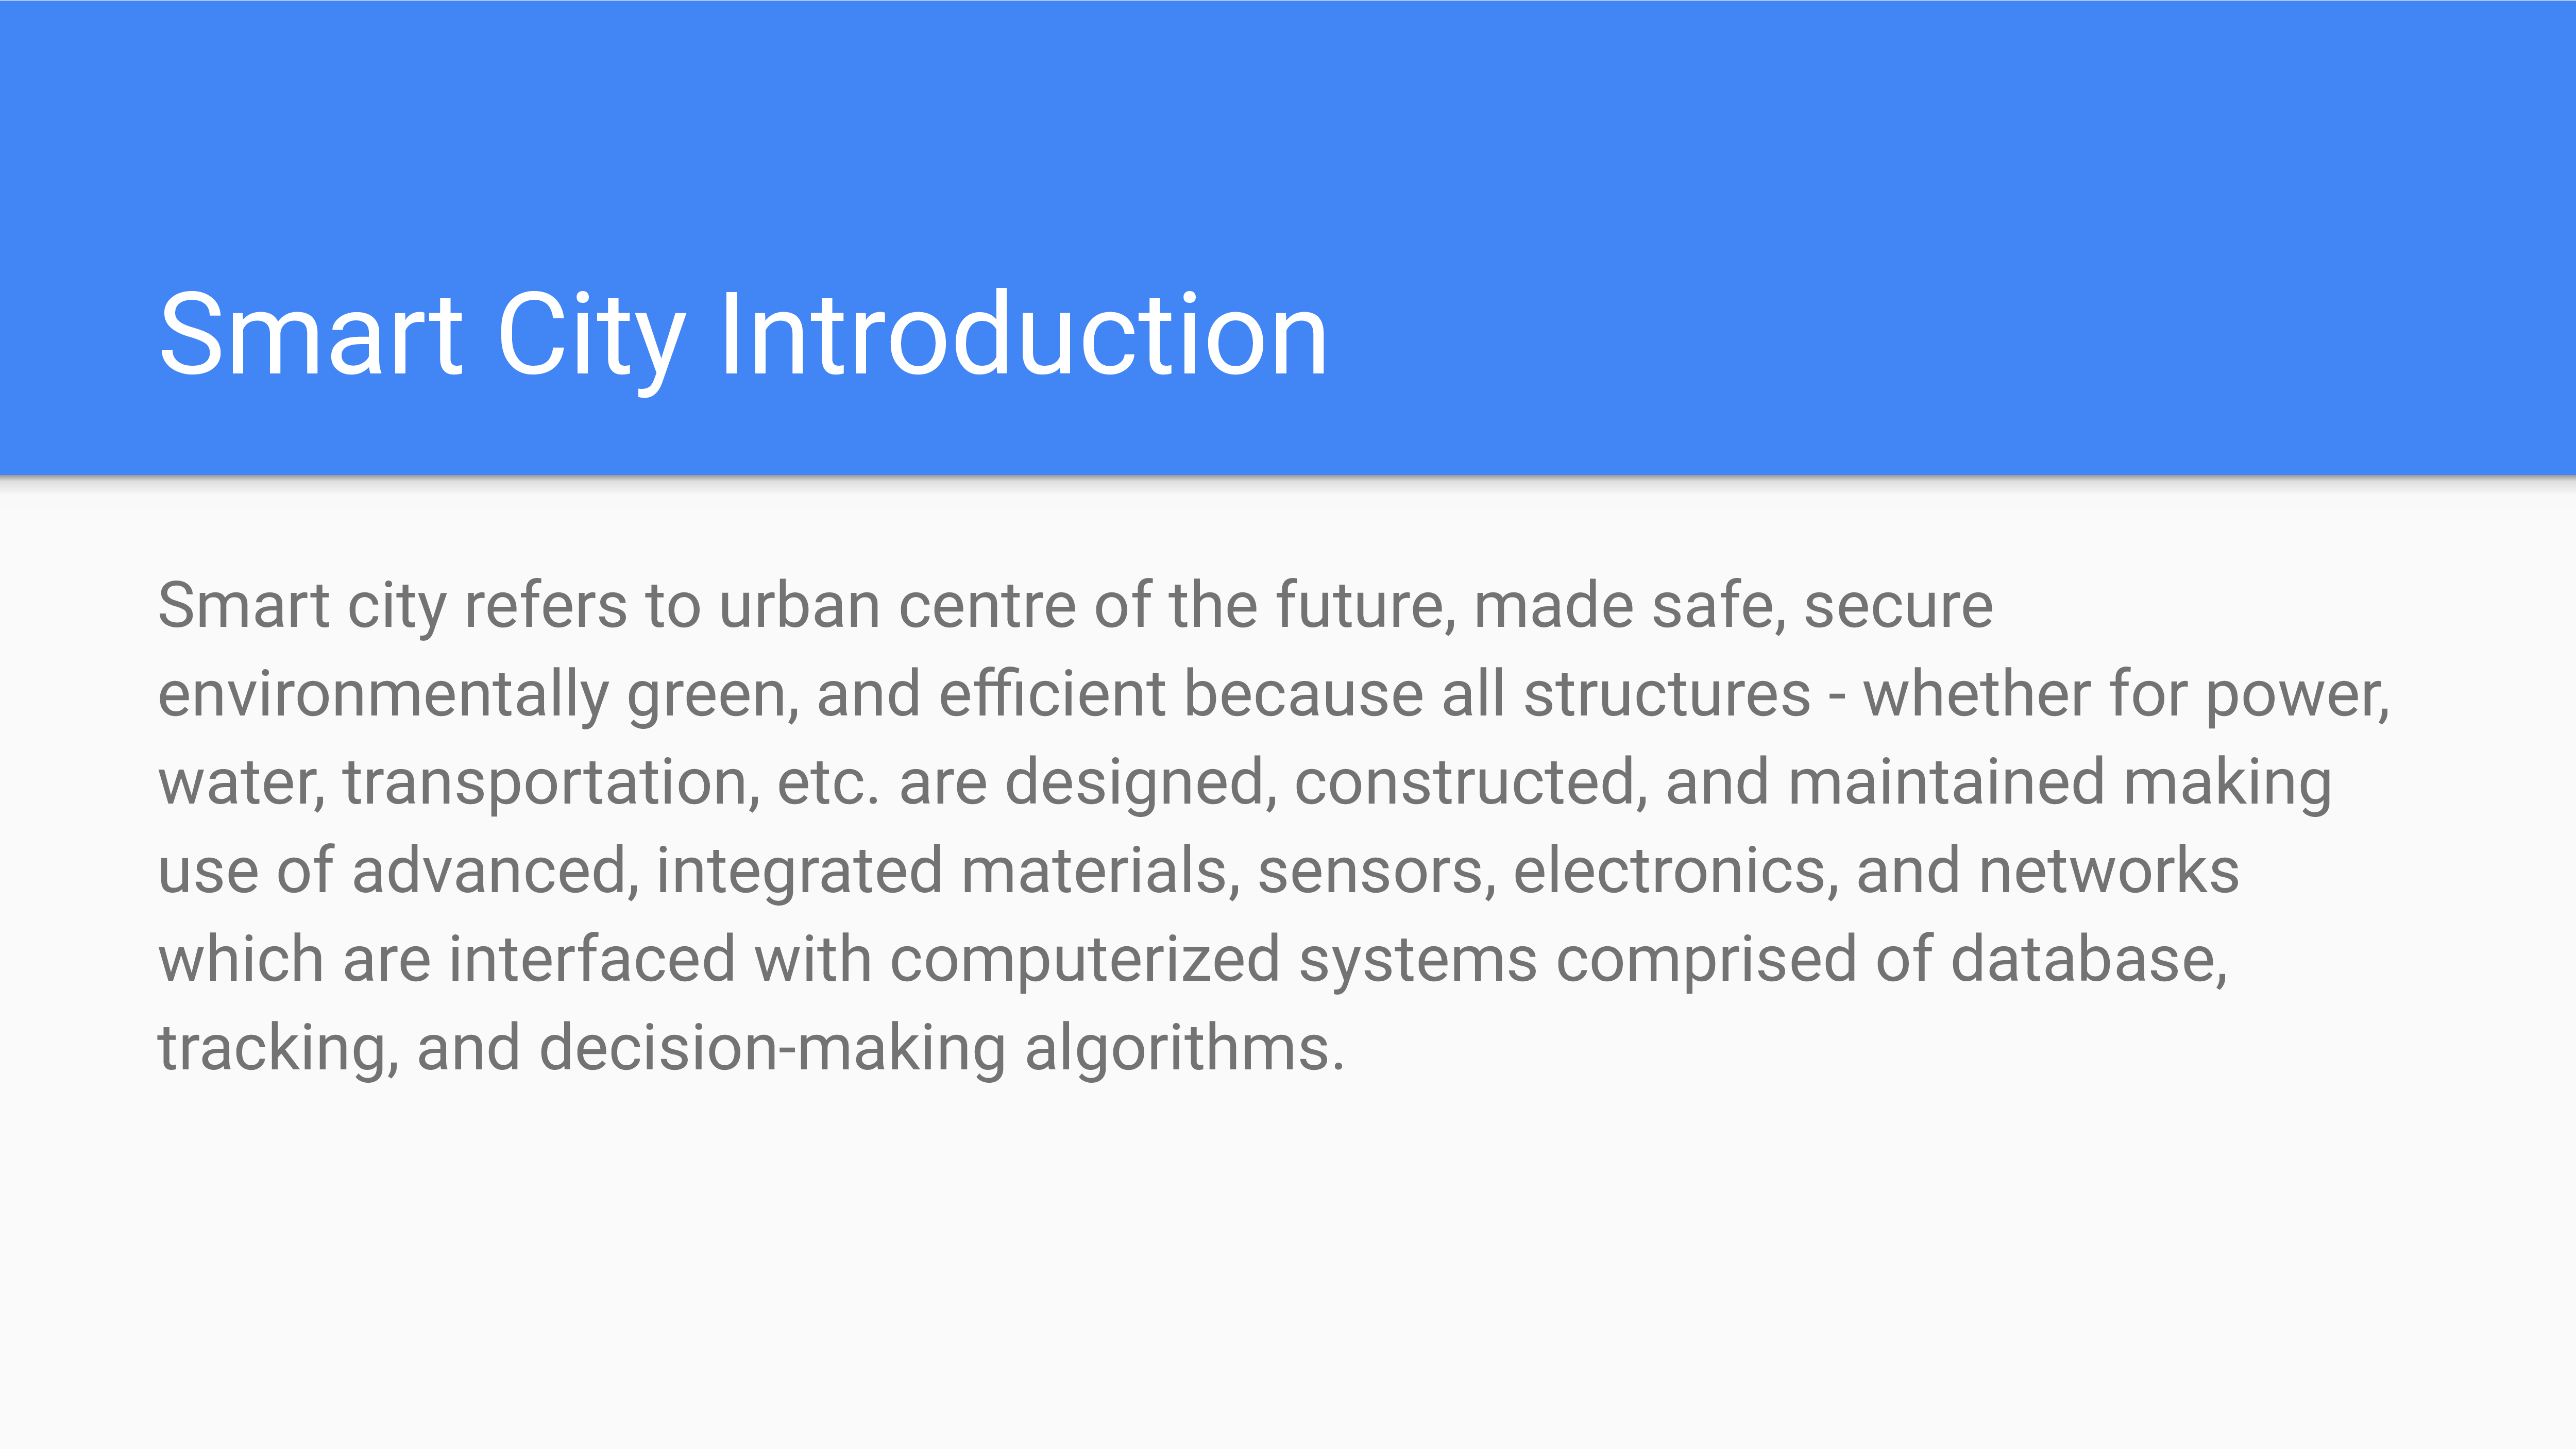
\includegraphics[width=0.7\linewidth]{./scrot/smart-city-2.png}
	\includegraphics[width=0.7\linewidth]{./scrot/smart-city-3.png}
\end{center}
\begin{center}
	\includegraphics[width=0.7\linewidth]{./scrot/smart-city-4.png}
	\includegraphics[width=0.7\linewidth]{./scrot/smart-city-5.png}
	\includegraphics[width=0.7\linewidth]{./scrot/smart-city-6.png}
	\includegraphics[width=0.7\linewidth]{./scrot/smart-city-7.png}
\end{center}

\subsection{Network Topology}
\begin{center}
	\includegraphics[width=0.7\linewidth]{./scrot/network-0.png}
	\includegraphics[width=0.7\linewidth]{./scrot/network-1.png}
	\includegraphics[width=0.7\linewidth]{./scrot/network-2.png}
	\includegraphics[width=0.7\linewidth]{./scrot/network-3.png}
\end{center}
\begin{center}
	\includegraphics[width=0.7\linewidth]{./scrot/network-4.png}
	\includegraphics[width=0.7\linewidth]{./scrot/network-5.png}
	\includegraphics[width=0.7\linewidth]{./scrot/network-6.png}
	\includegraphics[width=0.7\linewidth]{./scrot/network-7.png}
\end{center}


\section{Project work on Ms Access}

\subsection{Customer Table}
\includegraphics[width=1\textwidth]{./scrot/customer.png}

\subsection{Orders Table}
\includegraphics[width=1\textwidth]{./scrot/order.png}

\subsection{Book Table}
\includegraphics[width=1\textwidth]{./scrot/book.png}

\subsection{Relationship among Table}
\includegraphics[width=1\textwidth]{./scrot/relation.png}

\subsection{First name of Customer}
\includegraphics[width=\textwidth]{./scrot/q2-1.png}

\subsection{Book written by abc}
\includegraphics[width=1\textwidth]{./scrot/q2-2.png}

\subsection{Books ordered by specific date}
\includegraphics[width=1\textwidth]{./scrot/q2-3.png}

\subsection{Report for particular customer}
\includegraphics[width=1\textwidth]{./scrot/report.png}

\subsection{Form for particular book}
\includegraphics[width=1\textwidth]{./scrot/form.png}

\end{document}
